\chapter{Results}
\label{ch:results}


\section{Evolution of Patterns}
\label{sec:pattern evolution}

This Section gives an overview how the EOF patterns change over the time, also comparing the differences of the two chosen climate scenarios, which represent the extremes of climate change handling.   

\subsection{Evolution of Encoded Variability}



\begin{figure}[htb]
  \begin{center}
    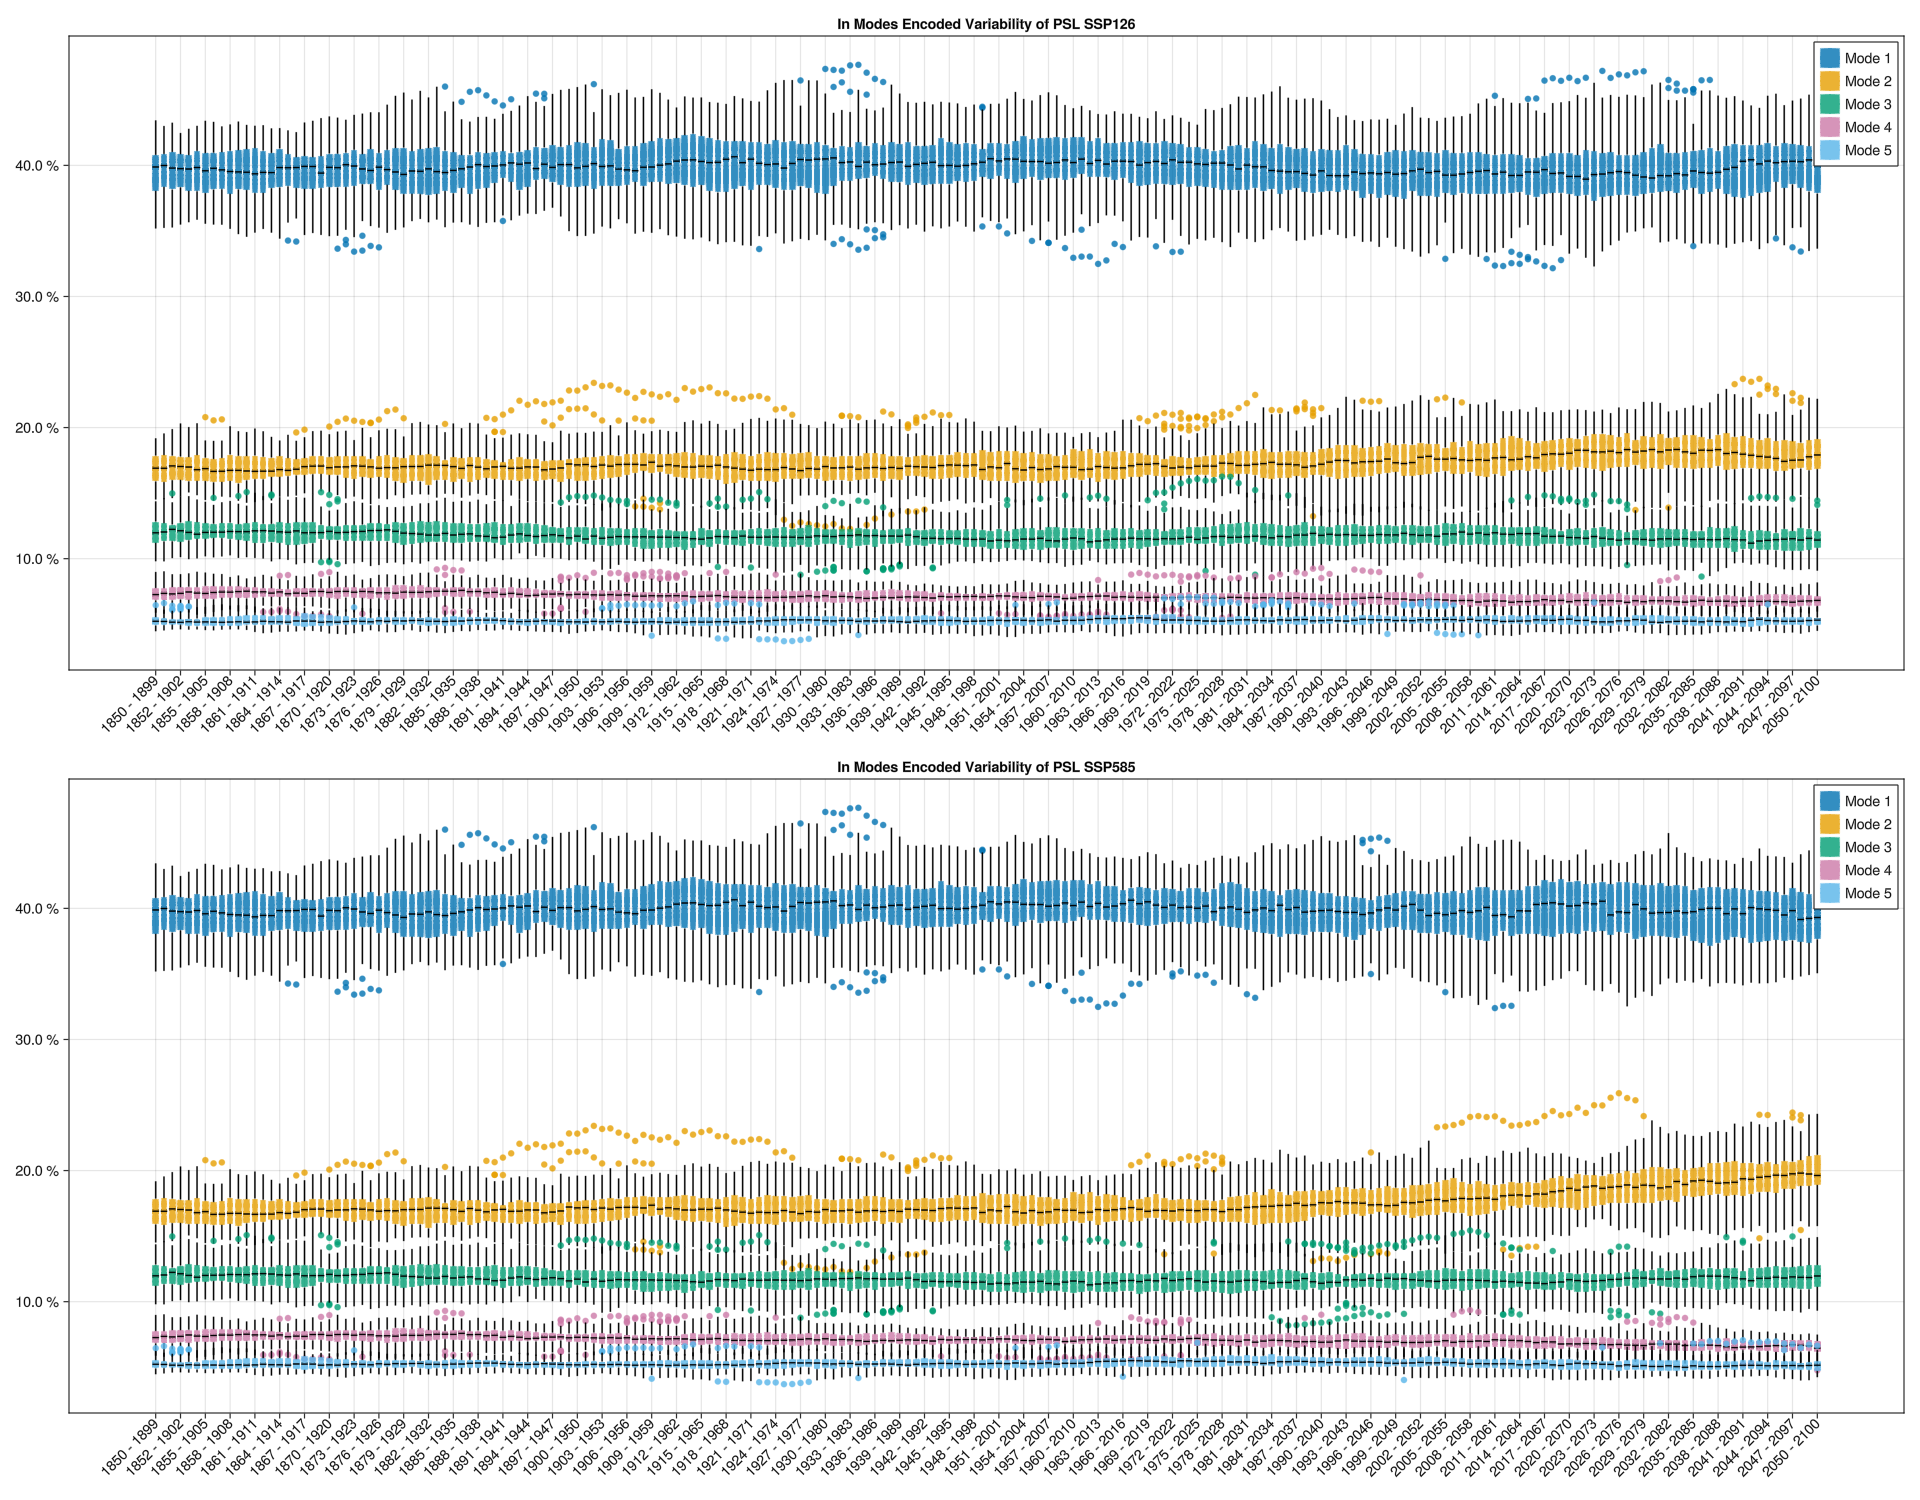
\includegraphics[width=0.85\textwidth]{figures/mode_variability_psl_50seasons.png}
  \end{center}
  \caption{Boxplot of the variability encoded in the top five modes of PSL EOF.}\label{fig:psl mode variability}
\end{figure}

The first simple evaluation is to look at the change of share of variability encoded by each EOF (see Equation~\ref{eq:eof variance calculation}). 
The results are displayed in boxplots, with the colored bar being $50\%$  of the members. 
The whiskers are 1.5 the size of the interquartile range (distance between upper and lower and of the colored bar), any data point outside that is considered an outlier and represented with dots. 


Figure~\ref{fig:psl mode variability} shows that there is no significant change in the SSP126 scenario in any way. 
The five most significant modes stay pretty much the same across the studied 250-year time period, with the primary mode (NAO) encoding around $39\%$ (median) of the whole dataset variability in each time scope, with fluctuations of the interquartile range ($50\%$ of the data) introduced by the members of the simulations being around $\pm 2\%$, with no significant trend over the years. 
The secondary mode (EAP) median stays around $17\%$, with the quartiles being $\pm 1\%$. 
The median variability encoded by EOFs 3,4 and 5 is around $13\%$, $8\%$, and $5\%$, respectively. 
Comparing it to the SSP585 scenario, it is obvious that there is very little to no change in Modes 3-5 and 1. 
But interestingly, the median variability encoded by the secondary mode rises from the $17\%$ in the 1850 - 1900 scope to around $20\%$ in the last one, exposing a clear trend over the course of climate change.   


\begin{figure}[hbt]
  \begin{center}
    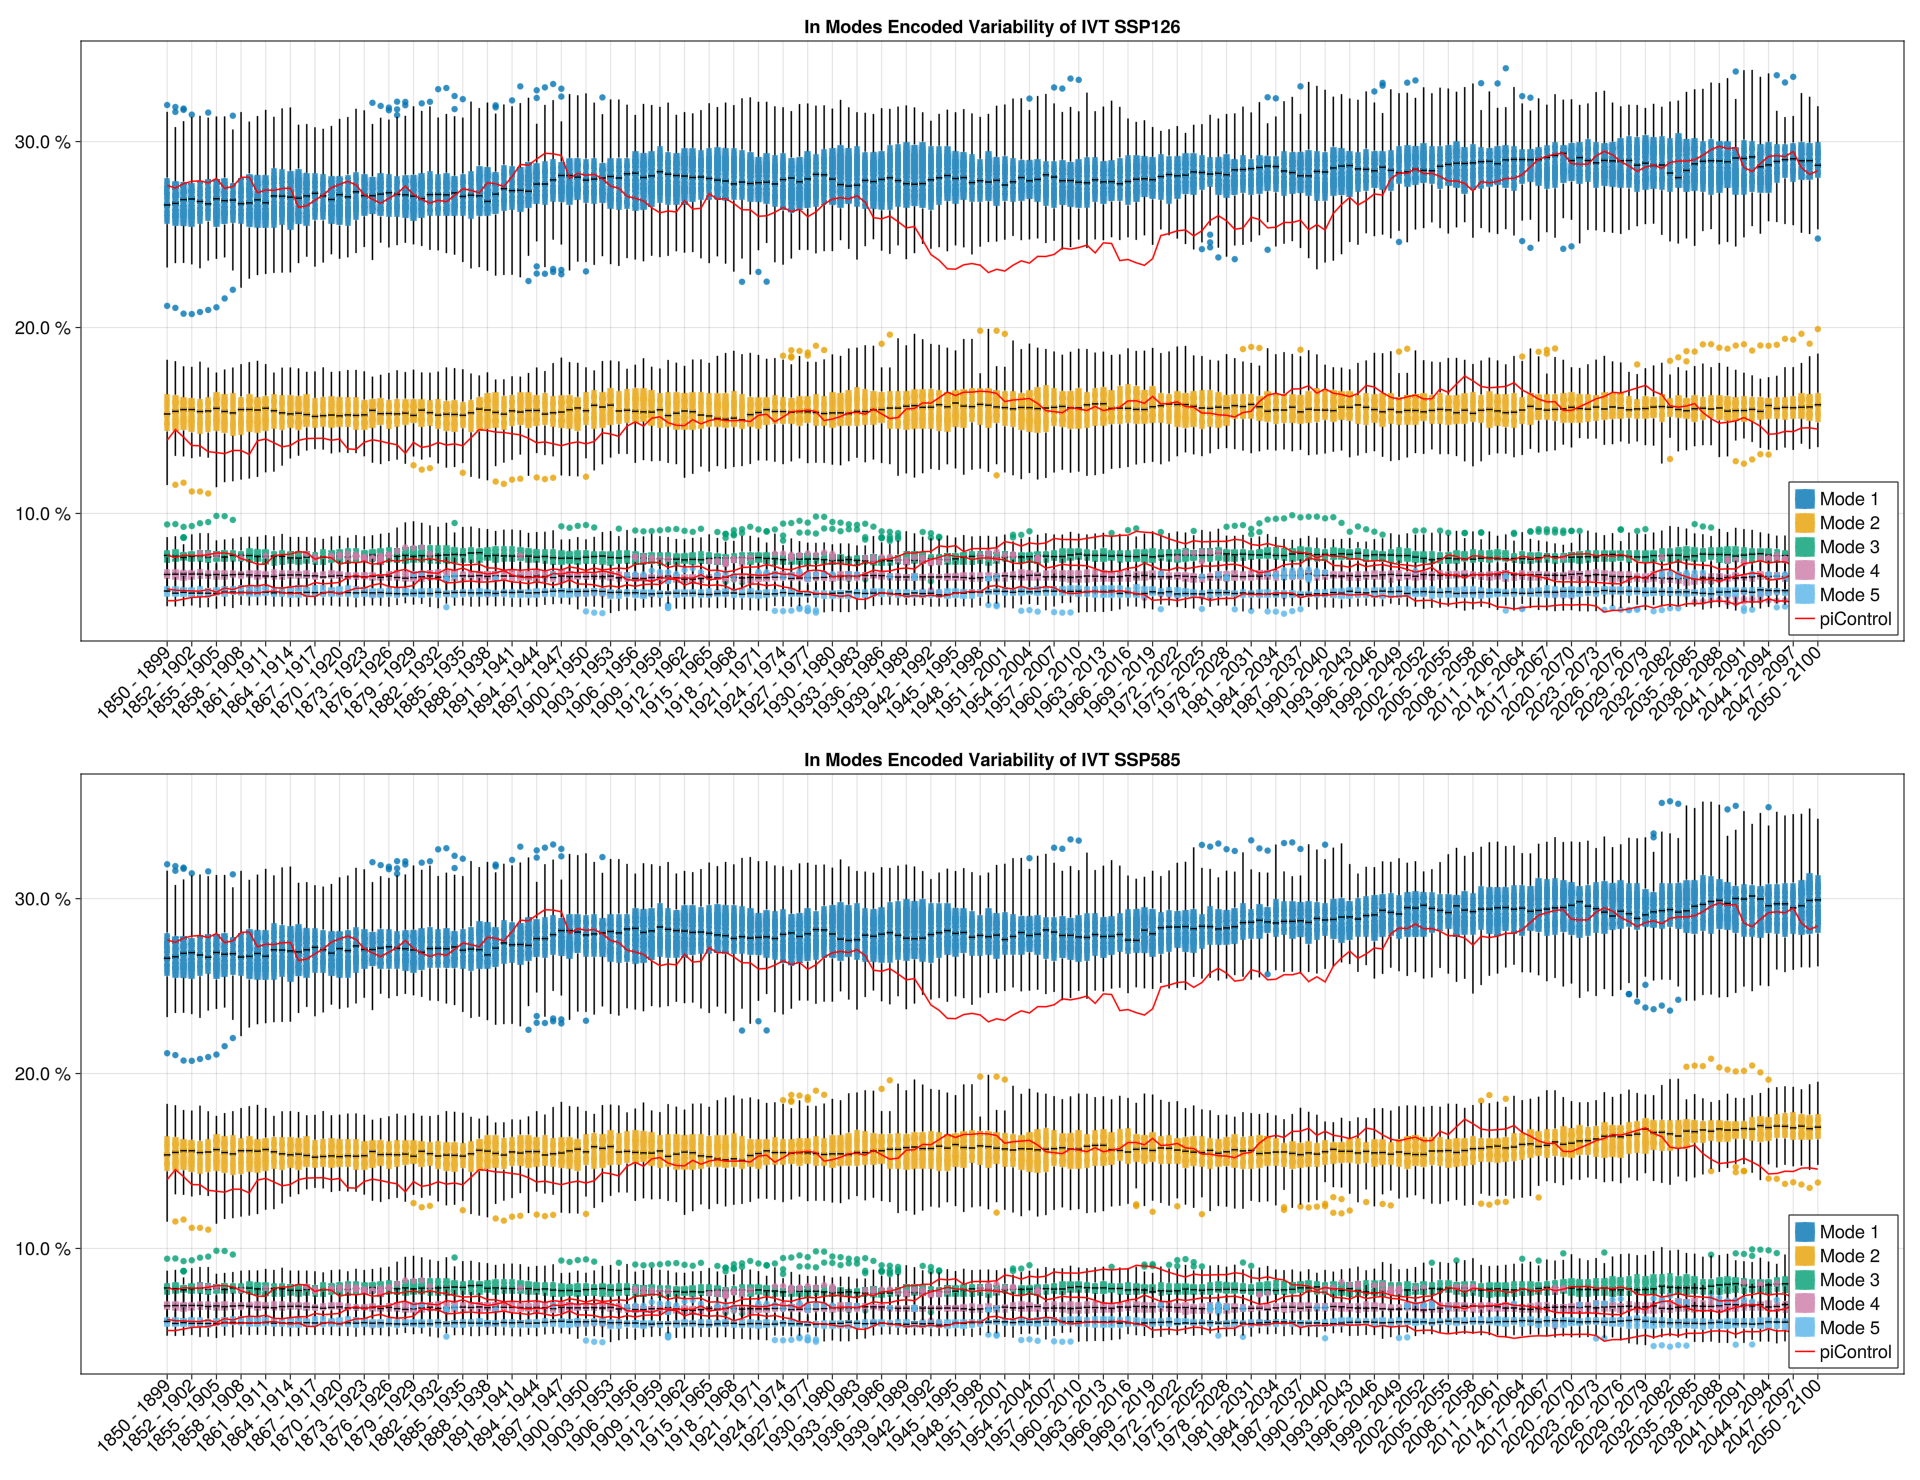
\includegraphics[width=0.85\textwidth]{figures/mode_variability_ivt_50seasons.png}
  \end{center}
  \caption{Same as Figure~\ref{fig:psl mode variability} but with IVT}\label{fig:ivt mode variability}
\end{figure}

The same analysis with the IVT patterns (Figure~\ref{fig:ivt mode variability}) reveal a general upwards trend in the primary mode of IVT, from median $26\%$ in the first window to around $28\%$ in the last. 
This trend is very similar in both SSP126 and SSP 585. 
Modes 3,4 and 5 also look very similar in both evaluated scenarios, with a median encoded variability of $8\%$, $6\%$, and $5\%$. 
Similar to Figure~\ref{fig:psl mode variability}, the secondary mode (representing around $15\%$ of variability) shows upward trend in scenario SSP585 to around $17\%$, which is not recognizable in the SSP126 scenario. 

\begin{figure}[htb]
  \begin{center}
    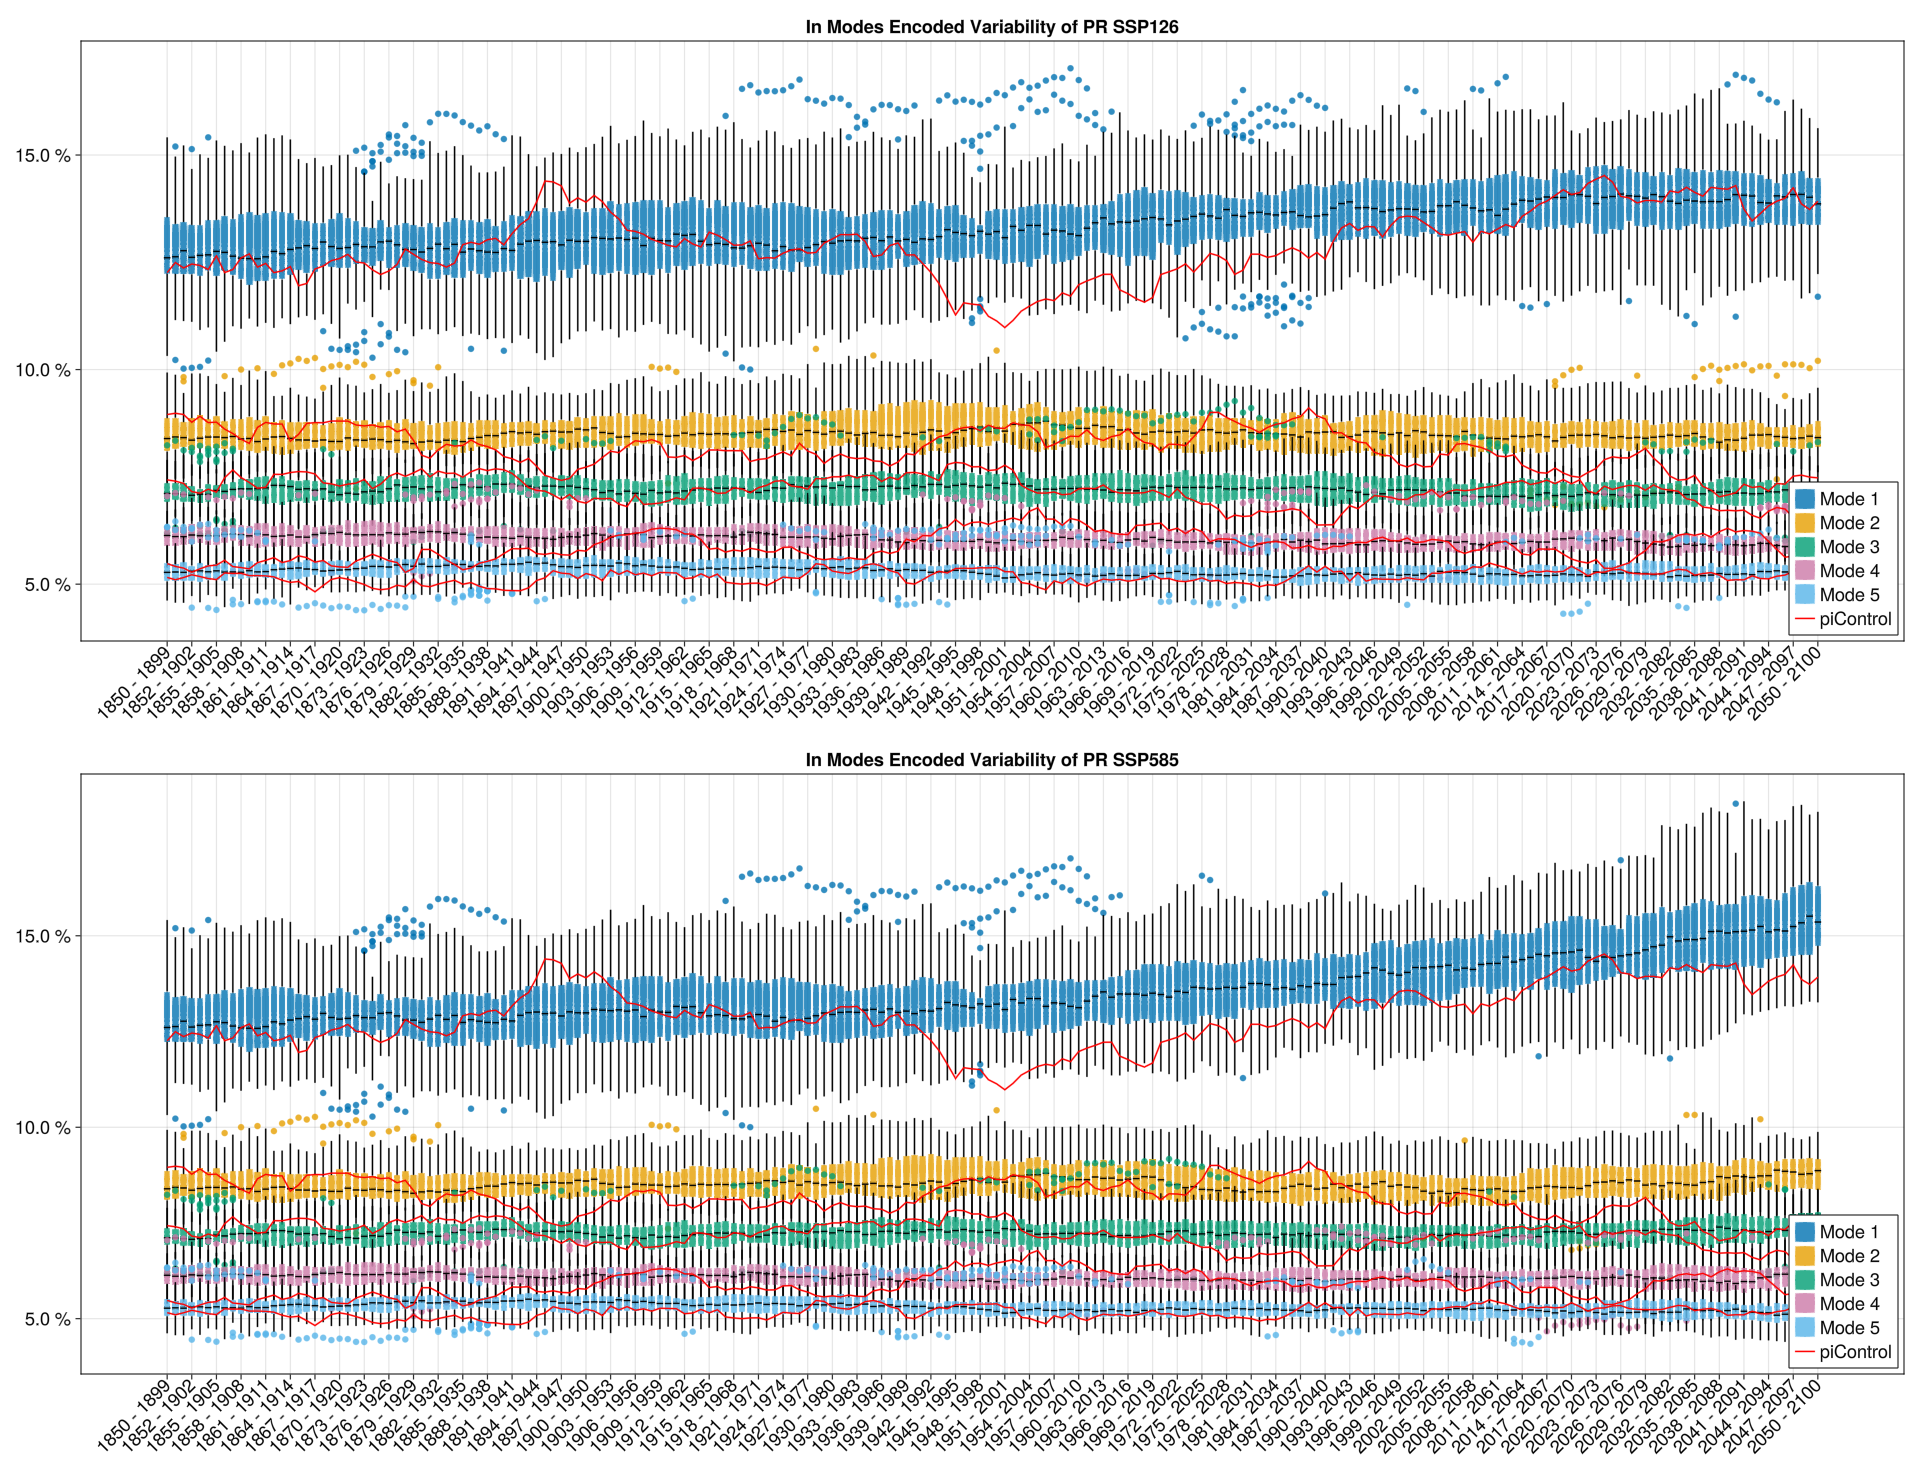
\includegraphics[width=0.85\textwidth]{figures/mode_variability_pr_50seasons.png}
  \end{center}
  \caption{Same as Figure~\ref{fig:psl mode variability} but with precipitation}\label{fig:pr mode variability}
\end{figure}

The comparison of mode variability evolution of precipitation EOFs (Figure~\ref{fig:pr mode variability}) shows no significant changes of modes 3,4, and 5 between both evaluated scenarios. 
Those encode on median $5\%$, $6\%$ and $6.5\%$ with small fluctuations introduced by the members. 
Mode 2 also looks very similar in both scenarios, with a median encoded variability of around $8.5\%$. 
The primary EOF on the other shows significant differences across scenarios: While it has a far greater variability across members then the other modes and follows a general upwards trend in both SSP126 and SSP585, it is more pronounced in the latter. 
It evolves from around $12.5\%$ in the 1850-1900 window to around $14\%$ in SSP126 and $15.5\%$ in SSP585.  


\subsection{Evolution of Spatial Patterns}

This Section shows the evolution of the spatial EOF patterns, shown in Figure~\ref{fig:5modes each variable}. 
Since the EOF modes four and five are generally quite low and similar in their eigenvalues (which directly correspond to the variance (see Equation~\ref{eq:eof variance calculation}) encoded shown in Figures~\ref{fig:ivt mode variability}, \ref{fig:psl mode variability}, and \ref{fig:pr mode variability}), they are left out of the analysis of this and the following sections, as modes' eigenvalues need to be well separated from each other \cite{hannachi_empirical_2007}. 
Usually, the rule of thumb introduced by \citeauthorwork{north_sampling_1982} is used, but since the eigenvalues of the first three modes (or two for precipitation, see Figure~\ref{fig:pr mode variability}), this is left out of this Thesis. 

The variability introduced through the 50 members of the MPI GE CMIP6 is displayed here with the hexbin approach explained in Section~\ref{sec:vis_analysis}, while a discussion of the hexbin visualization compared to the classical spaghetti is given in Section~\ref{sec:discussion}.
The images in this section are the first and last frame from the video displaying the evolution of the different scenarios.\todo{Reference the videos somehow}  


\begin{figure}[htb]
  \begin{center}
    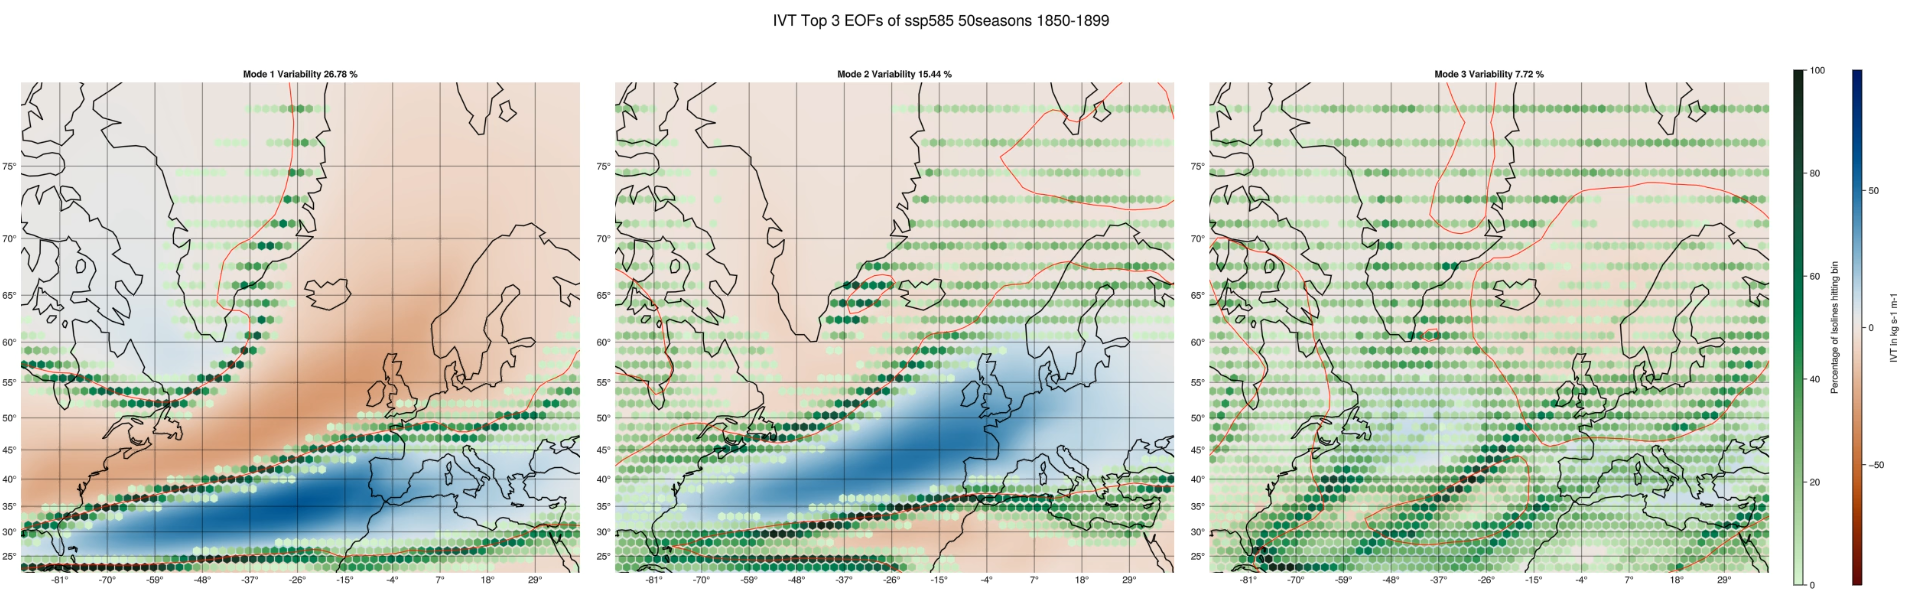
\includegraphics[width=0.85\textwidth]{figures/ivt_spat_patterns_hexbin_18501899_ssp585_50seasons.png}
    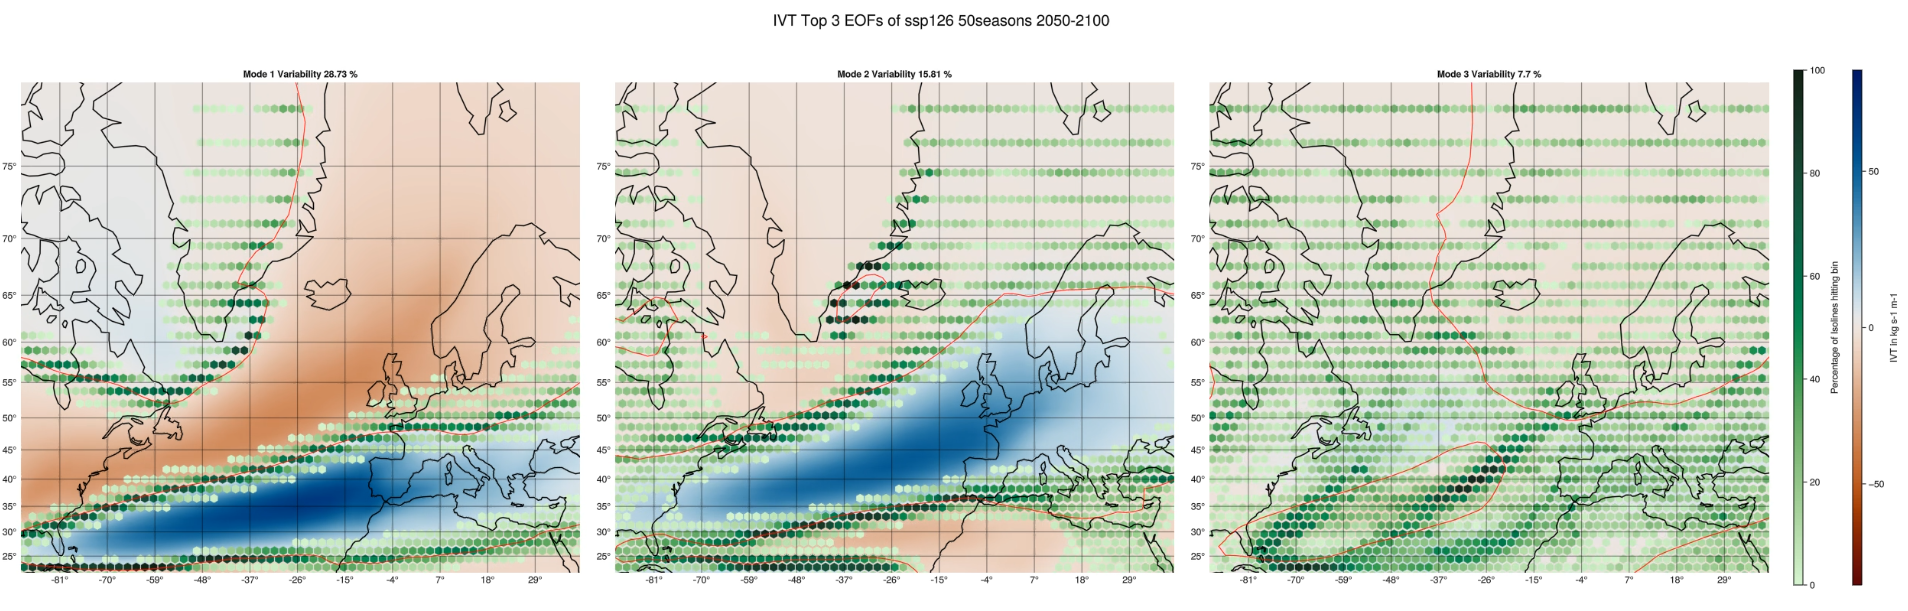
\includegraphics[width=0.85\textwidth]{figures/ivt_spat_patterns_hexbin_20502100_ssp126_50seasons.png}
    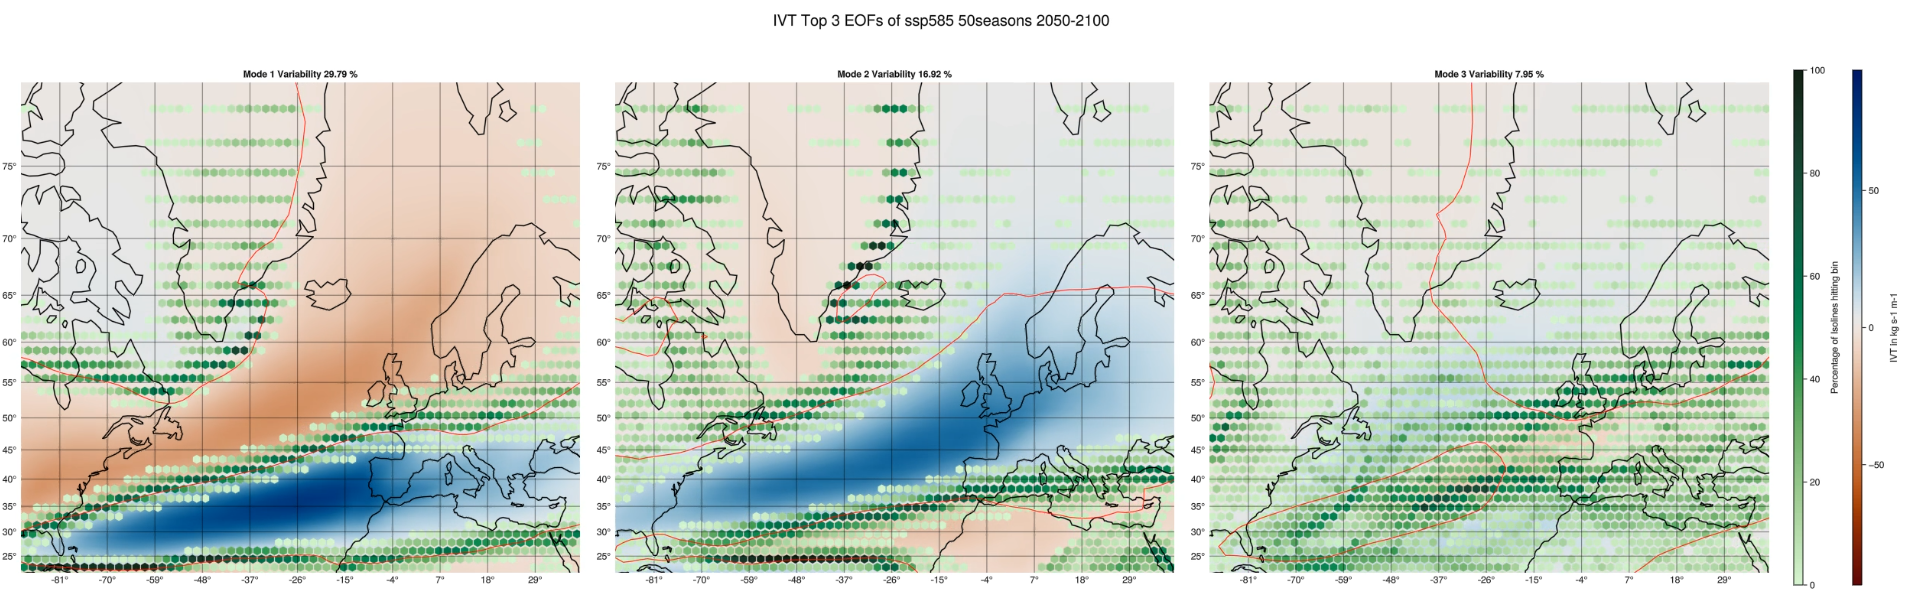
\includegraphics[width=0.85\textwidth]{figures/ivt_spat_patterns_hexbin_20502100_ssp585_50seasons.png}
  \end{center}
  \caption{The top three EOFs of IVT data, with a 50 winter scope and hexbins visualizing the variability introduced by simulation members. The top row displays the state in the historical simulation (second half of 19th century), while middle (SSP126) and bottom (SSP585) display the state in the second half of the 21st century. The red line shows the contour line of zero of the preindustrial control simulation. }\label{fig:ivt eof evolution}
\end{figure}

Figure~\ref{fig:ivt eof evolution} shows the evolution of IVT EOF spatial patterns. 
In general, regardless of the future scenario, EOF1 and EOF2 stays structurally very stable across all the ensembles' members, which can be seen on the clear, dark green borders of the colored surfaces. 
EOF3 on the other hand seems pretty unstable, since most of the map is covered in light greed hexagons, which means that the contour lines of zero switch significantly between all the 50 members of the ensemble. 
This also has consequences for the alignment across members and time, which will obviously not work if the patterns differ greatly across time and members. 
Therefor, the analysis regarding such patterns will be kept short since the multi-member, sliding window analysis of such patterns used in this Thesis does not apply very well to such patterns. 

The dominant EOF1 pattern of IVT is characterized by a positive IVT values reaching from Florida to Spain and negative values from the USA east coast to Northern Europe and the Northern Atlantic. 
There are three, clearly visible borders of these positive and negative areas, associated with three groups of contour lines: The first going through Canada, quite coherently across members (many dark green hexagons in a row), and then following the east coast of Greenland, fading out over the mainland quite differently across the members (many light green hexagons in a larger area). 
The second border follows a similar pattern: Starting quite coherent across members at the beginning of the Florida peninsula, over the Atlantic to the east coast of France, and then fading out differently in Eastern Europe. 
The third border goes through the most southern part of the evaluated area, through North Africa and then to the Arabian Peninsula, staying pretty consistent across its path. 
Comparing the state of the patterns at the end of the different future scenario simulations, the change is quite subtle but visible in the area of France and the South of the British Islands:
While the dark green hexagons in the beginning of the historical simulation are on/below the red line of the preindustrial simulation, the majority of zero contour lines in SSP126 seem to be above the preindustrial control contour line. 
In SSP585, the dark green hexagons stretch even further north, indicating that the slight northward shift of IVT EOF1 at the end of the 21st century is even more pronounced. 

The IVT EOF2 is characterized by a strong IVT anomaly right were the seperation contour line of EOF1 is, and lesser, opposite anomalies in the north and south. 
Comparing the beginning of the historical simulation with SSP126, the changes seem only minimal, whereas the difference of SSP585 and the others are far more pronounced: 
While the southern, prominent separation contour line seems to experience a slight shift to the north, the norther isoline appears to move to the east, opening the pattern up to the north. 
Also the big area of fading out contour lines in the north of Scandinavia, seems to now be (more or less) uniformly part of the positive anomaly.  
% While the border in Greenland looks very similar at the end of SSP126 and the begin of the historical simulation, 
% On this example a way of interpreting the hexbin visualization is given, which can be applied to the patterns in Figures \ref{fig:pr eof evolution} and \ref{fig:psl eof evolution}. 




\begin{figure}
  \begin{center}
    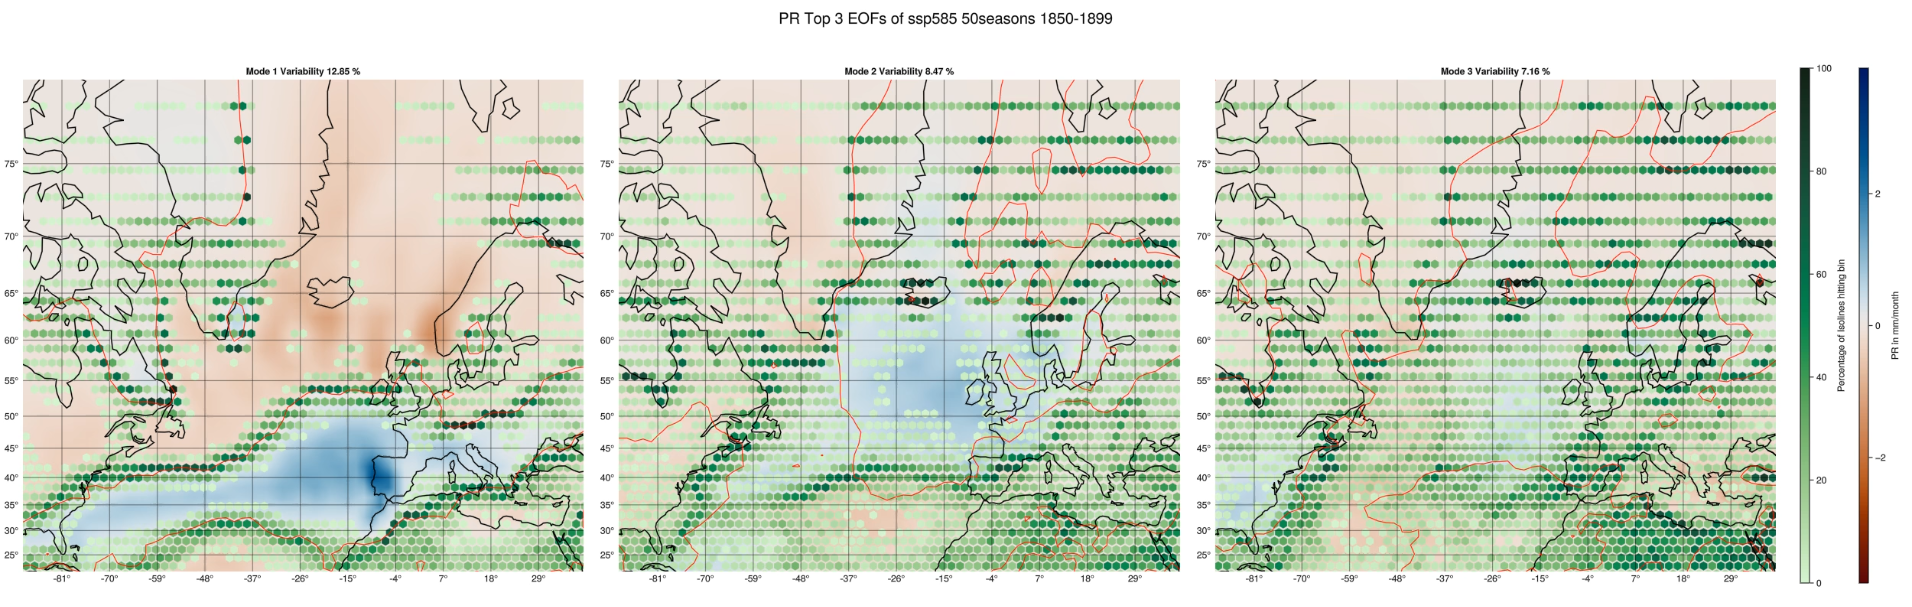
\includegraphics[width=0.95\textwidth]{figures/pr_spat_patterns_hexbin_18501899_ssp585_50seasons.png}
    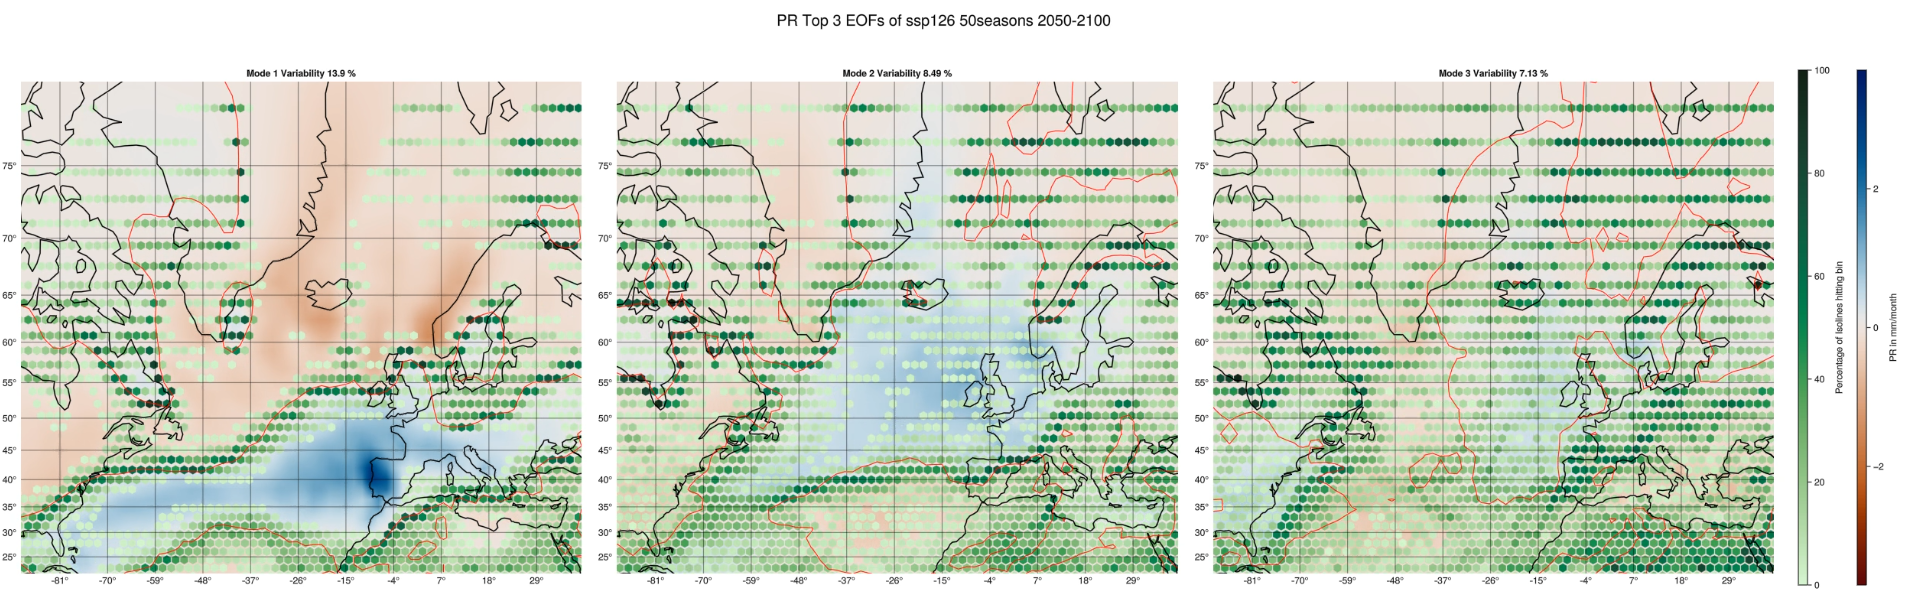
\includegraphics[width=0.95\textwidth]{figures/pr_spat_patterns_hexbin_20502100_ssp126_50seasons.png}
    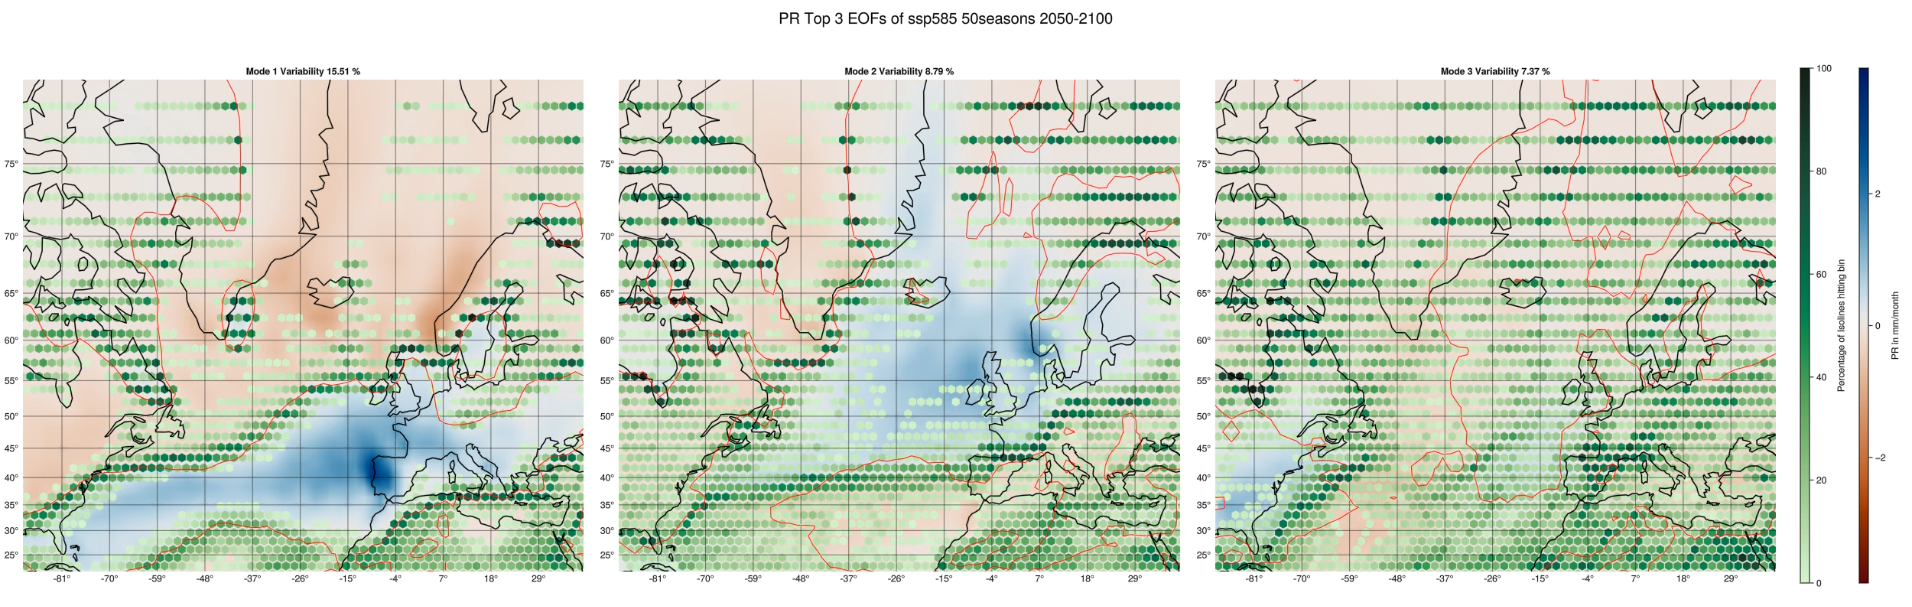
\includegraphics[width=0.95\textwidth]{figures/pr_spat_patterns_hexbin_20502100_ssp585_50seasons.png}
  \end{center}
  \caption{Same as Figure~\ref{fig:ivt eof evolution}, but with precipitation data.}\label{fig:pr eof evolution}
\end{figure}

\begin{figure}
  \begin{center}
    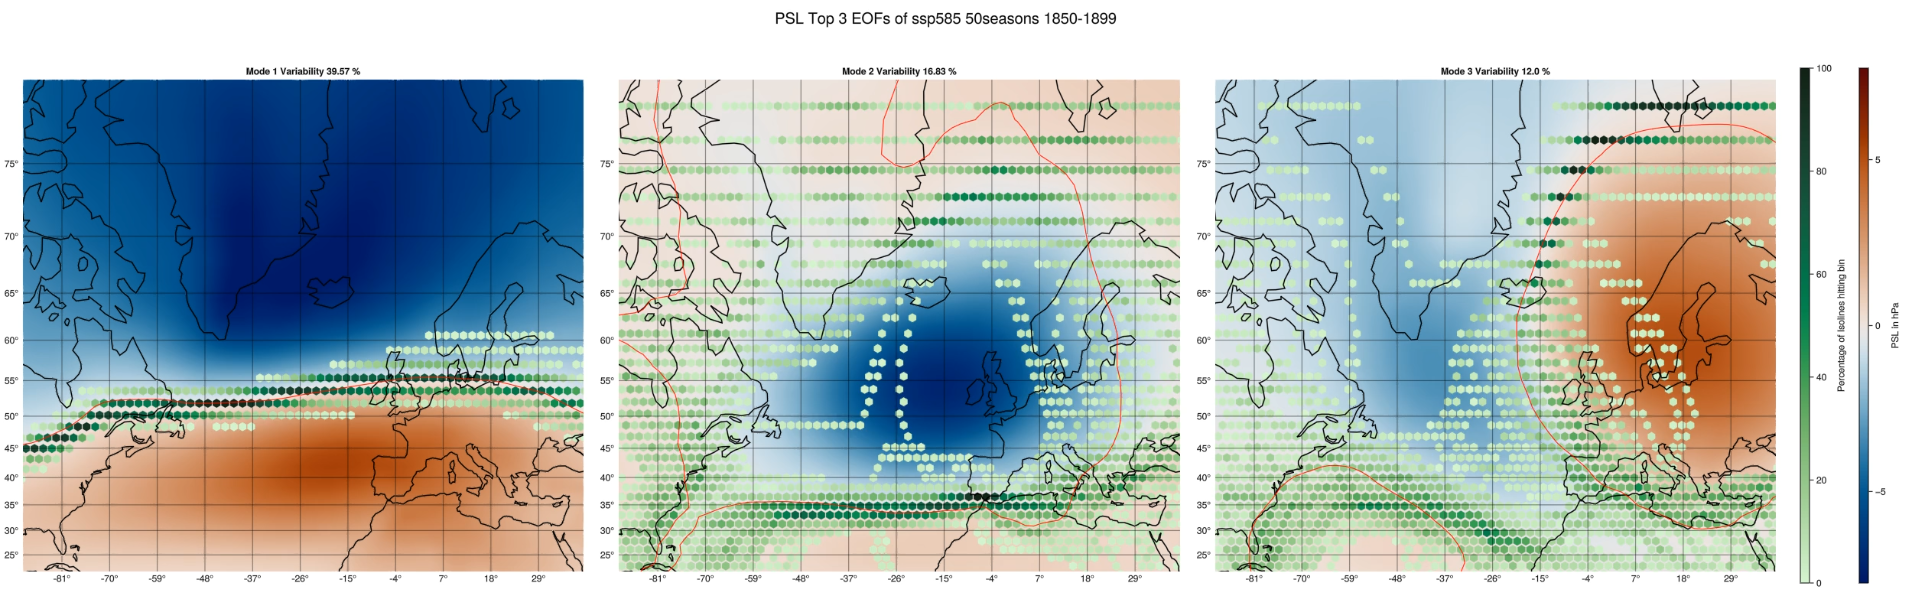
\includegraphics[width=0.95\textwidth]{figures/psl_spat_patterns_hexbin_18501899_ssp585_50seasons.png}
    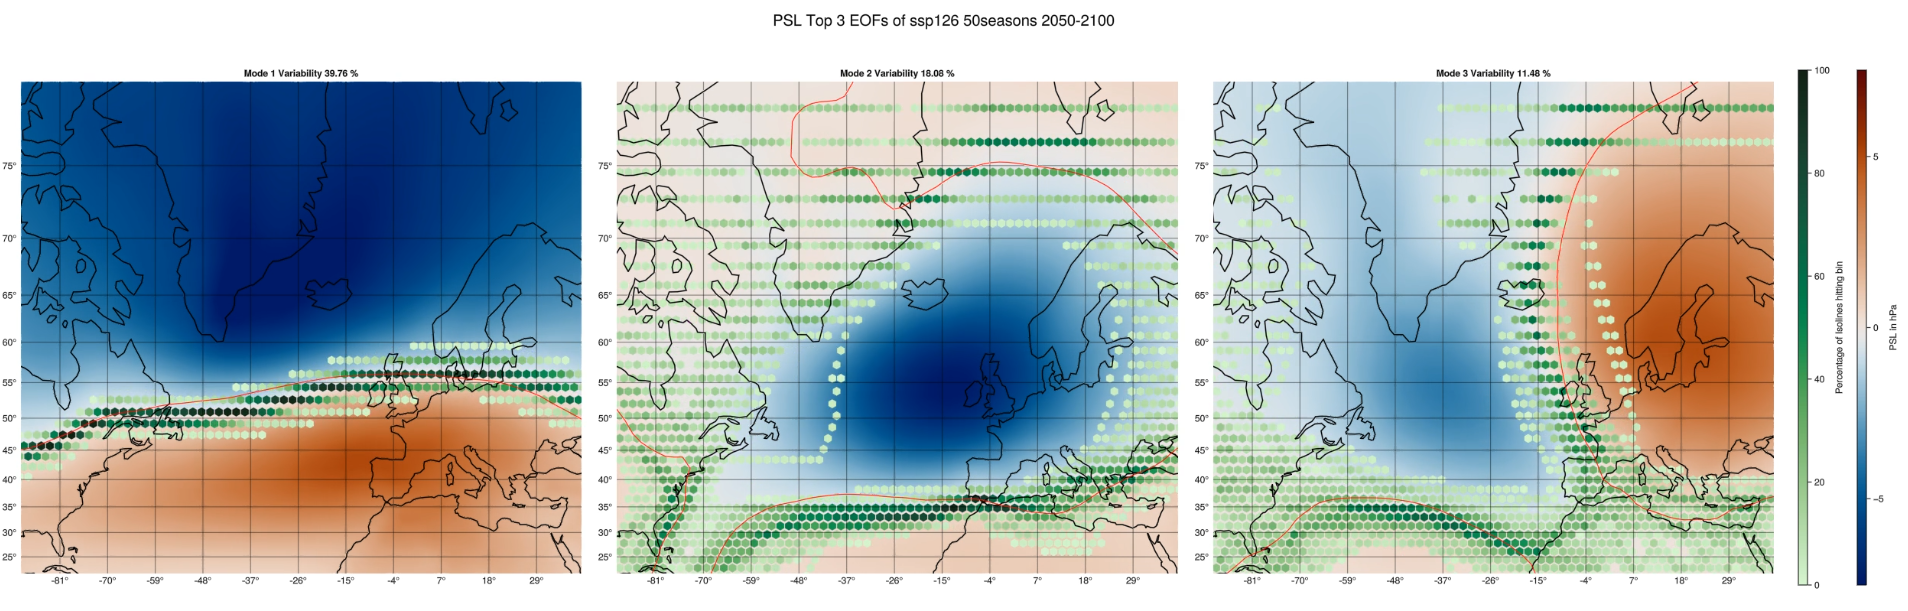
\includegraphics[width=0.95\textwidth]{figures/psl_spat_patterns_hexbin_20502100_ssp126_50seasons.png}
    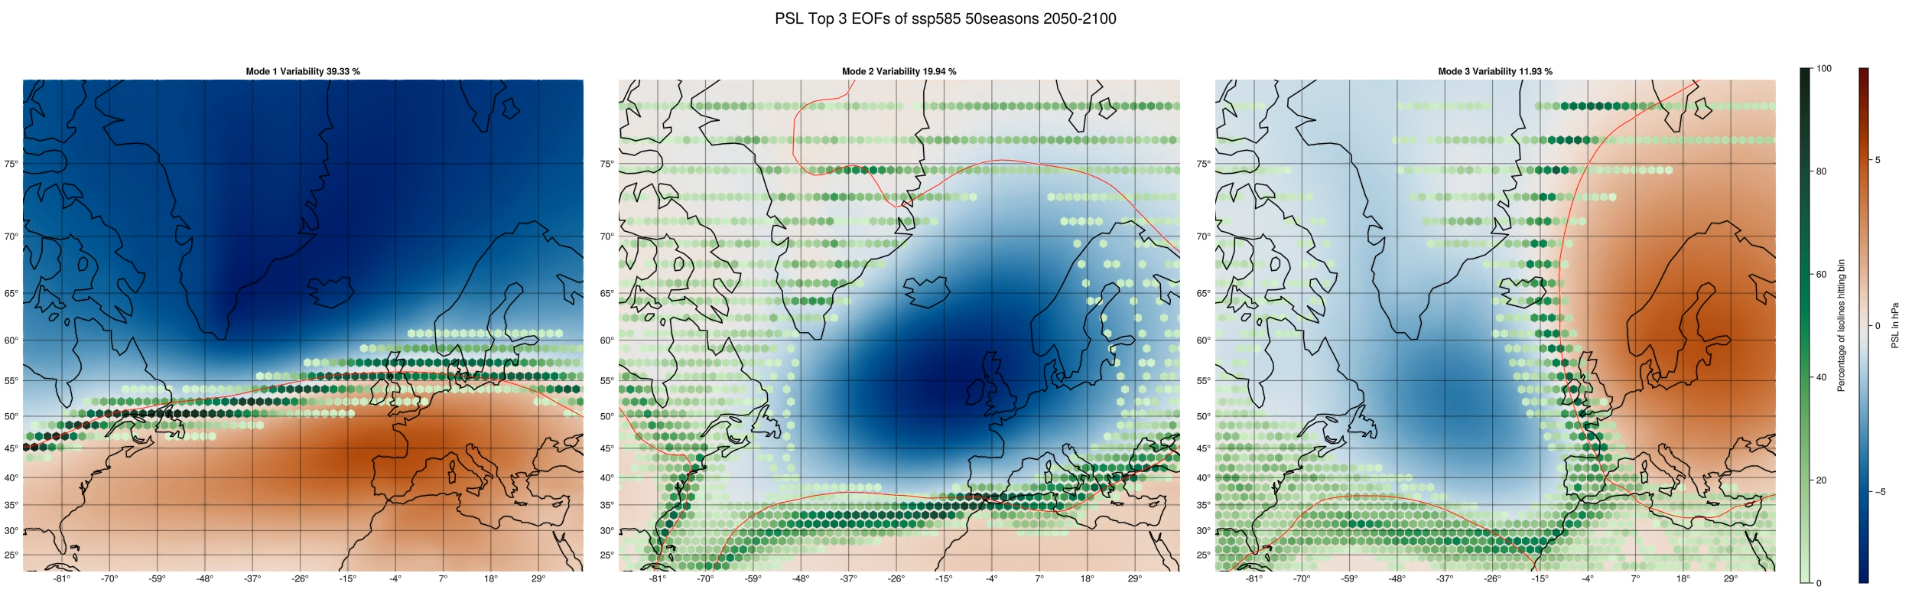
\includegraphics[width=0.95\textwidth]{figures/psl_spat_patterns_hexbin_20502100_ssp585_50seasons.png}
  \end{center}
  \caption{Same as Figure~\ref{fig:ivt eof evolution}, but with sea level pressure data.}\label{fig:psl eof evolution}
\end{figure}


\subsection{Evolution of Temporal Patterns}


As already explained in Section~\ref{sec:vis_analysis}, there is no proper way to visualize the EOF coefficients of an ensemble in the same way related work did it. 
Therefor, the only way left is to analyze statistics of those signals and compare them in a boxplot to get a sense of variability across members. 
In the Figures~\ref{fig:std ivt evolution}, \ref{fig:std psl evolution}, and \ref{fig:std pr evolution} the evolution of the standard deviation (SD) of IVT, sea level pressure, and precipitation is displayed, respectively. 
Keep in mind that being scaled to the original unit means multiplying each EOF coefficient series with the associated singular value, which is very closely related to the encoded variance (see Equation~\ref{eq:eof variance calculation}). 


\begin{figure}
  \begin{center}
    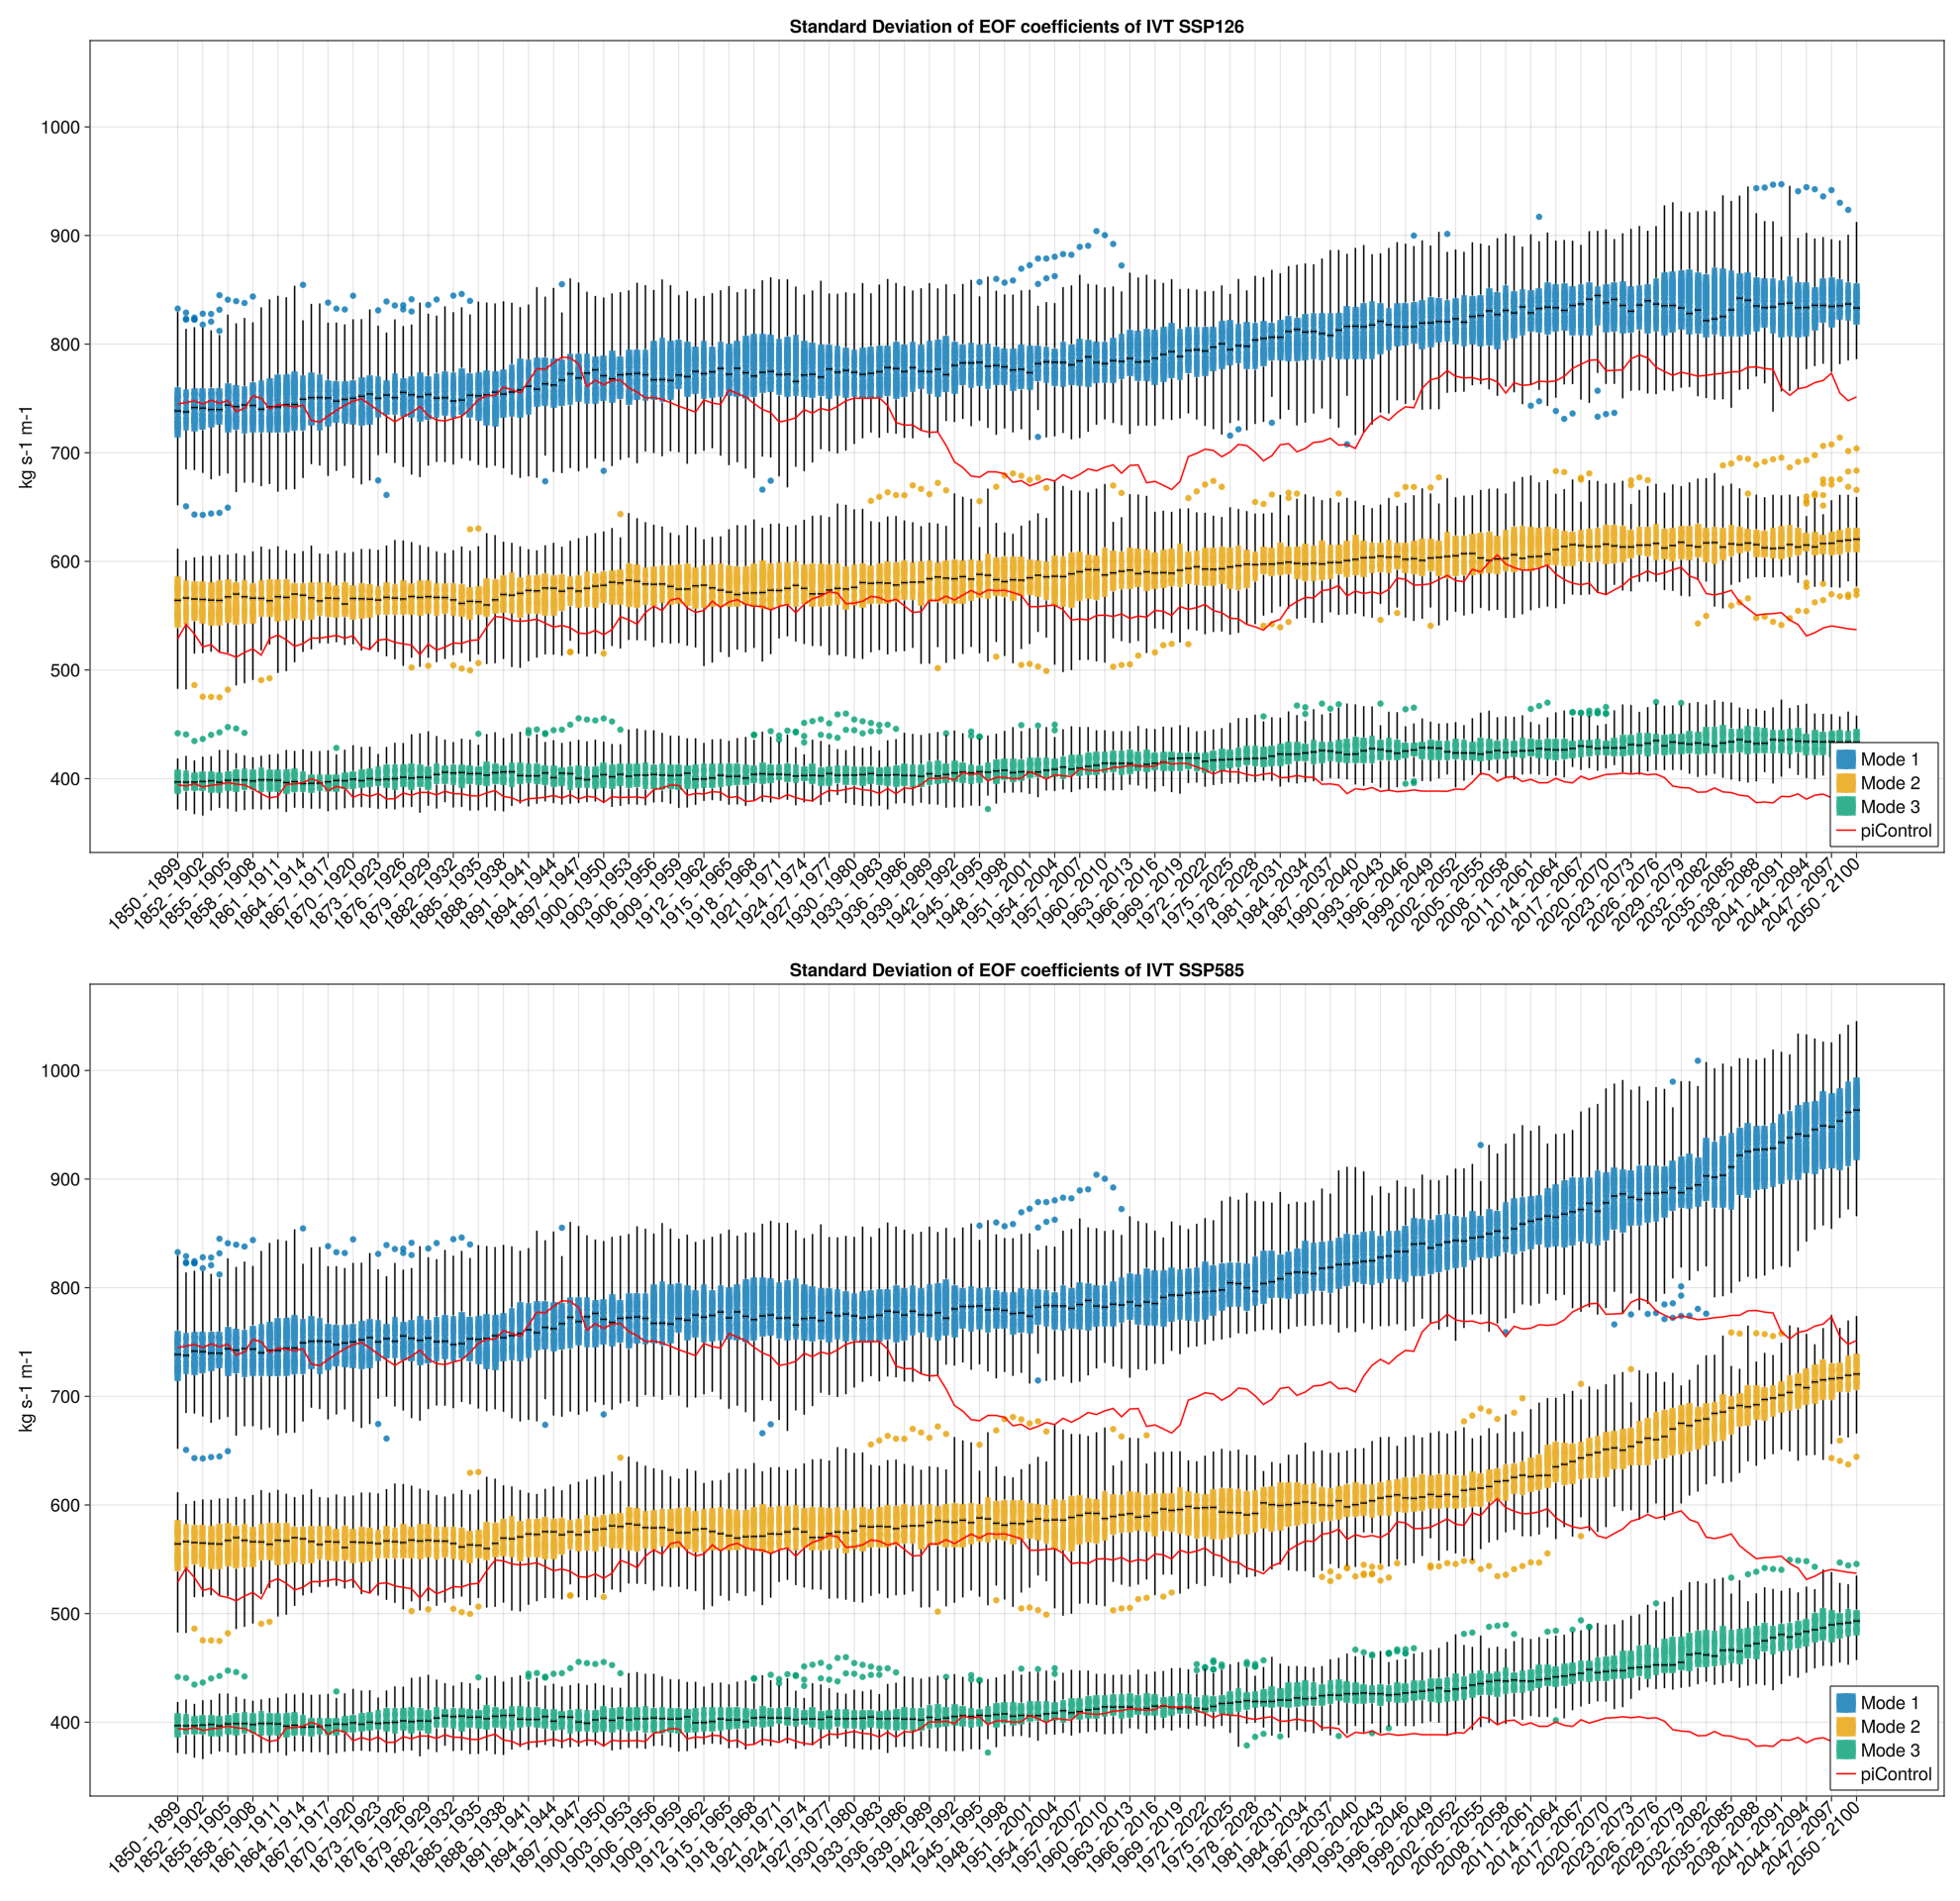
\includegraphics[width=0.75\textwidth]{figures/std_ivt_50seasons_tempmodescale_3modes.png}
  \end{center}
  \caption{Evolution of the standard deviation of IVT EOF coefficients for each scope and simulation member.}
  \label{fig:std ivt evolution}
\end{figure}

Analyzing the evolution of the standard deviation of the IVT EOF coefficients, that compared to the quasi-stationary preindustrial control simulation the SD increases significantly, regardless of scenario. 
While Mode one experiences a drop in SD in the scopes from $\approx$ 1933 to 1999 (start of the scope), the SD of the members keep steadily increasing. 
This increase is far more pronounced in the SSP585 scenario than in SSP126, culminating in a median SD of $\approx 970~kg~s^{-1} m^{-1}$ (compared to $\approx 820~kg~s^{-1}m^{-1}$ in SSP126). 
This change is far more extreme than the sole change of proportionate encoded variability shown in Figure~\ref{fig:ivt mode variability}. 
The variance across the members seems pretty similar in both scenarios. 
All of this applies to modes two and three as well: Slow but steady increase in SD, which stays consistent in SSP126 but experiences a sharp increase in the later scopes of SSP585.  


\begin{figure}
  \begin{center}
    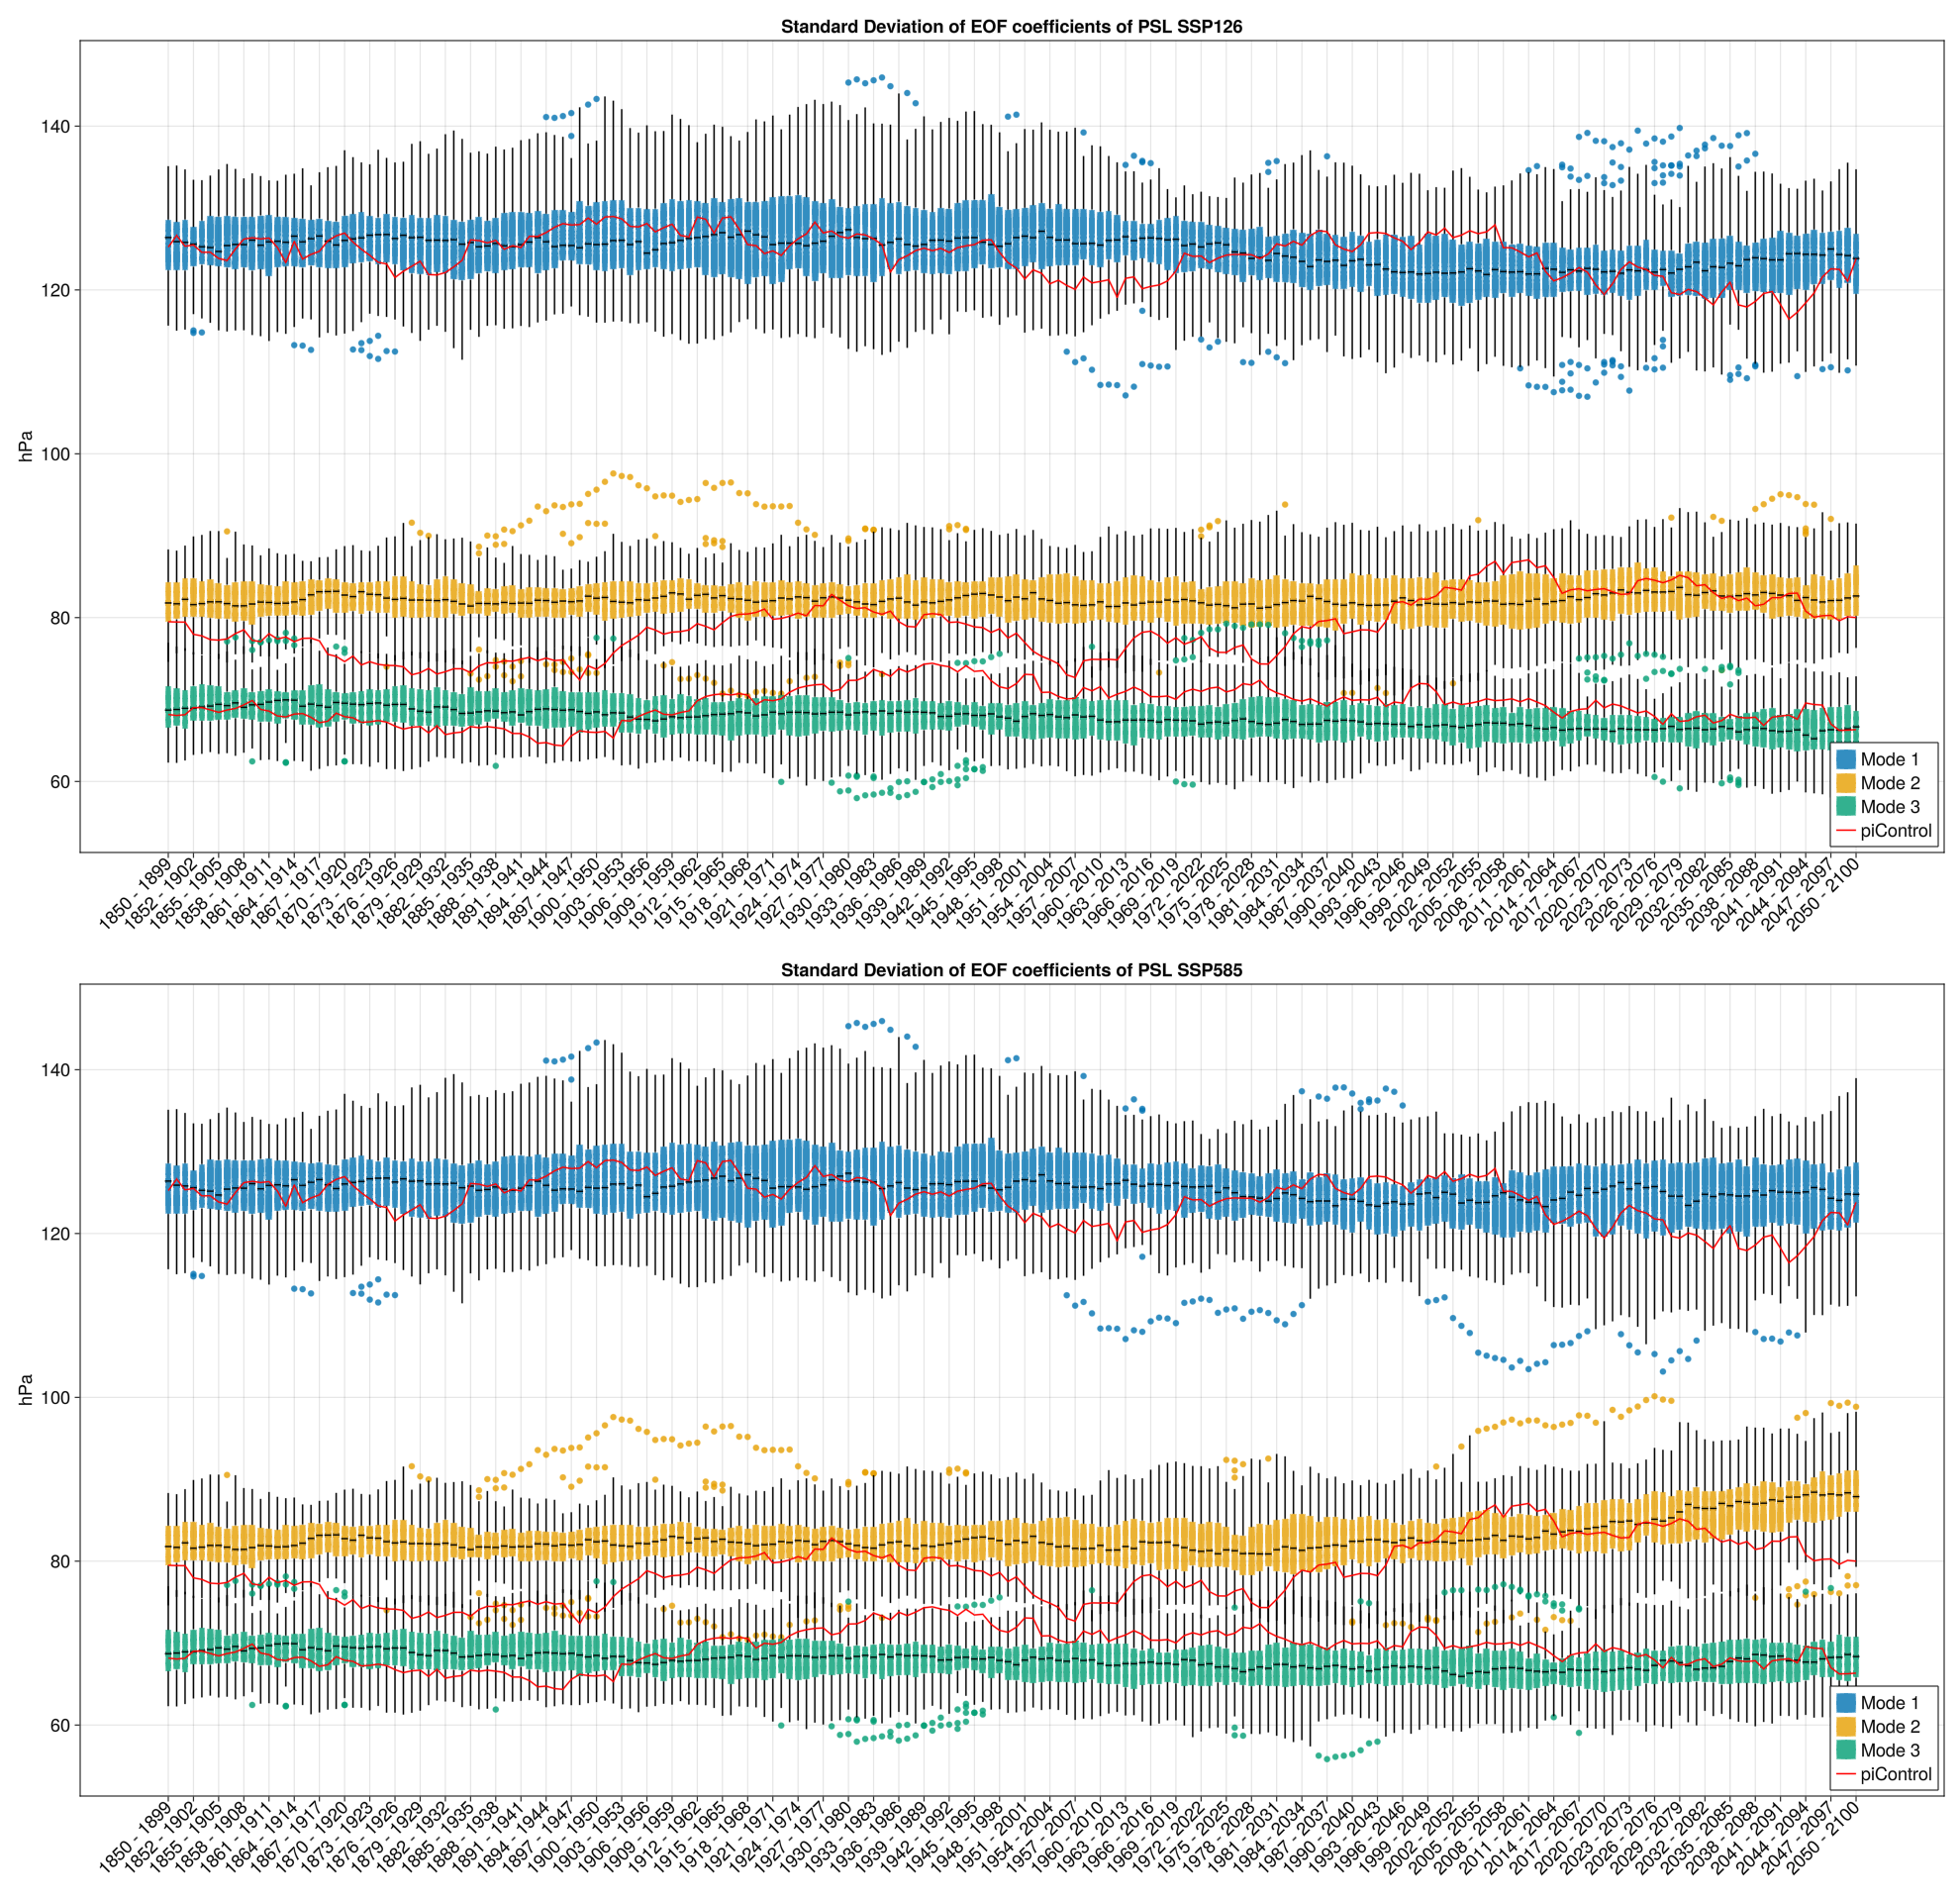
\includegraphics[width=0.75\textwidth]{figures/std_psl_50seasons_tempmodescale_3modes.png}
  \end{center}
  \caption{Same as Figure~\ref{fig:std ivt evolution}, but with sea level pressure data.}
  \label{fig:std psl evolution}
\end{figure}

Regarding the evolution of SD of sea level pressure EOF, it is obvious that the levels are more consistent over all the scopes, regardless of the scenario. 
Also, the piControl simulation is completely in line with the corresponding boxplots and could not be distinguished from the historical/scenario simulation. 
Comparing the scenarios, SD of Mode 1 coefficients (NAO indices) seem to be very similar to each other, with SSP585 having maybe a bit more variability across members. 
While it's also hard to distinguish the results of the different scenarios for Mode 3, SD evolution of Mode 2 (EAP indices) seem to experience a more pronounced increase in the later scopes in SSP585 than SSP126.  
This could be explained with the increase in proportional variability of that mode shown in Figure~\ref{fig:psl mode variability}.


\begin{figure}
  \begin{center}
    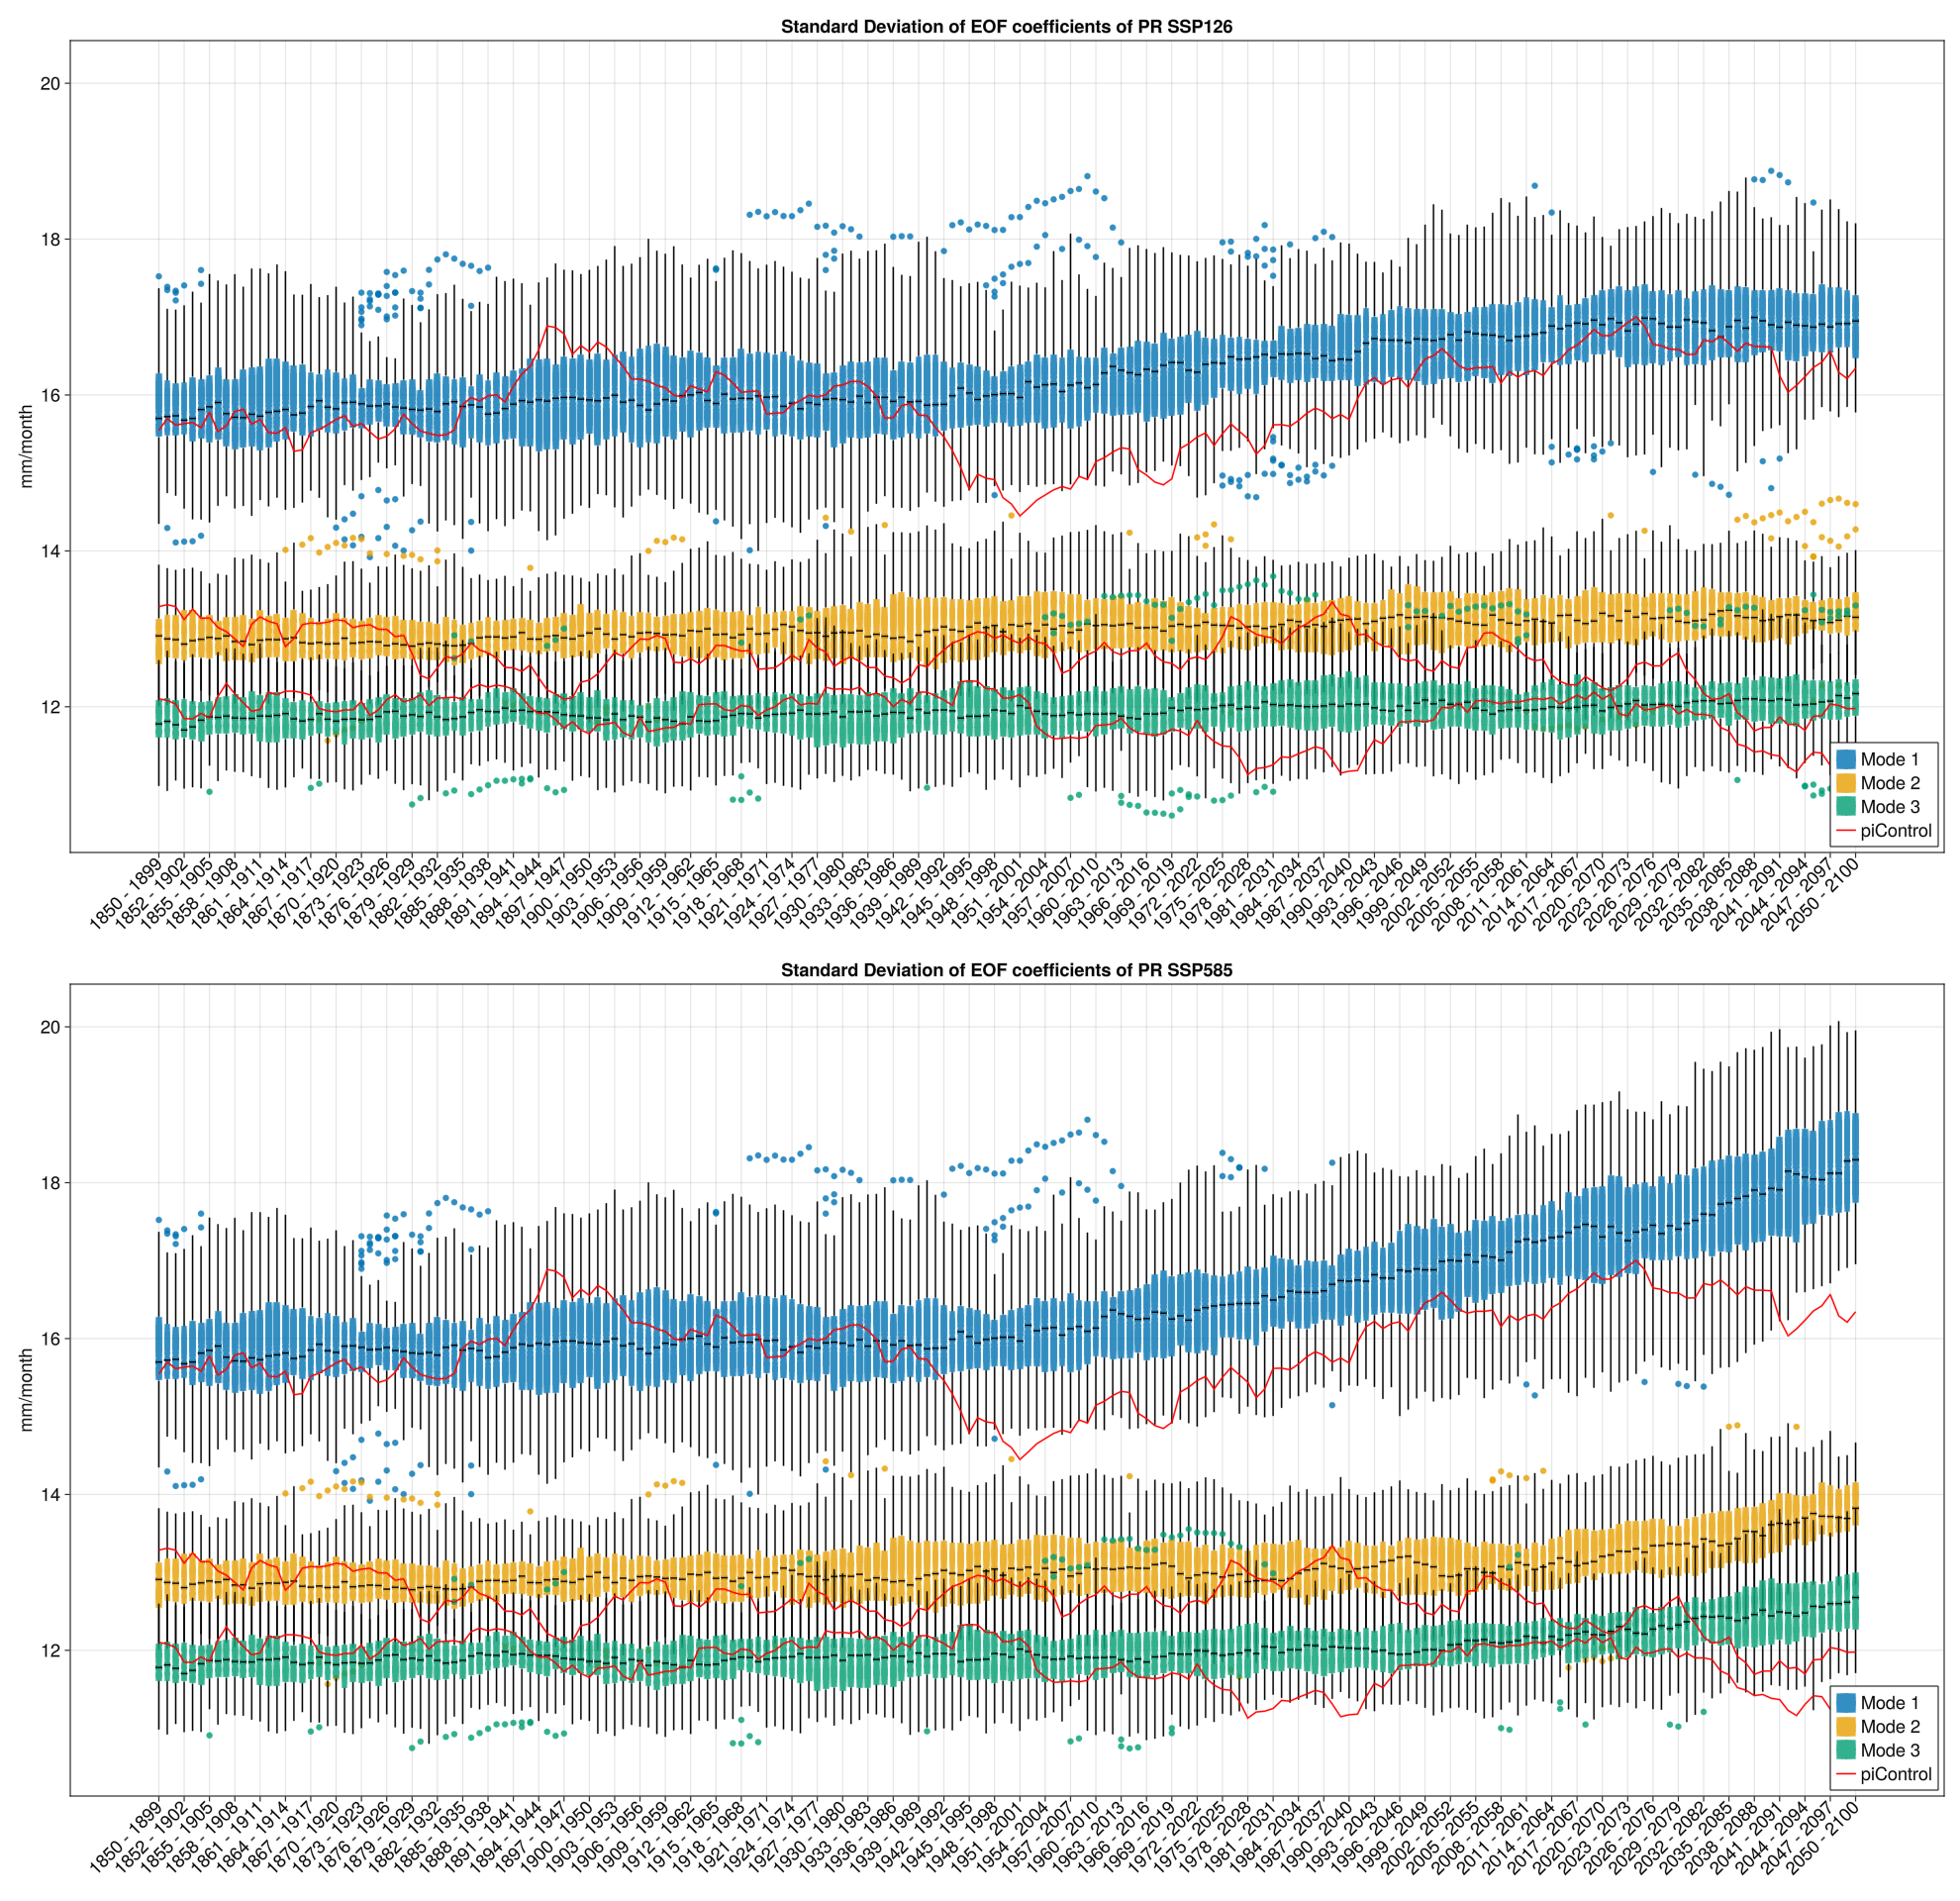
\includegraphics[width=0.75\textwidth]{figures/std_pr_50seasons_tempmodescale_3modes.png}
  \end{center}
  \caption{Same as Figure~\ref{fig:std ivt evolution}, but with precipitation data.}
  \label{fig:std pr evolution}
\end{figure}

The standard deviation of precipitation EOF coefficients seems to expose the largest differences in comparison to piControl simulation and the scenarios. 
Similarly to the IVT piControl EOF coefficients SD, the precipitation piControl has a dump in EOF coefficient SD in roughly the same timespan of scopes, which may be connected. 
The SSP126 scenario only shows a moderate increase in mode one, and no significant change in other modes. 
On the other hand, SSP585 shows a significant increase in all modes, which is different to the encoded variability shown in Figure~\ref{fig:pr mode variability}, where only the first mode exposes a steep increase. 



\section{Relationships with other Variables}



\subsection{Relationships of EOFs}


\subsubsection{Relationships of IVT and Sea Surface Pressure EOFS (NAO and EAP)}

\begin{figure}
  \begin{center}
    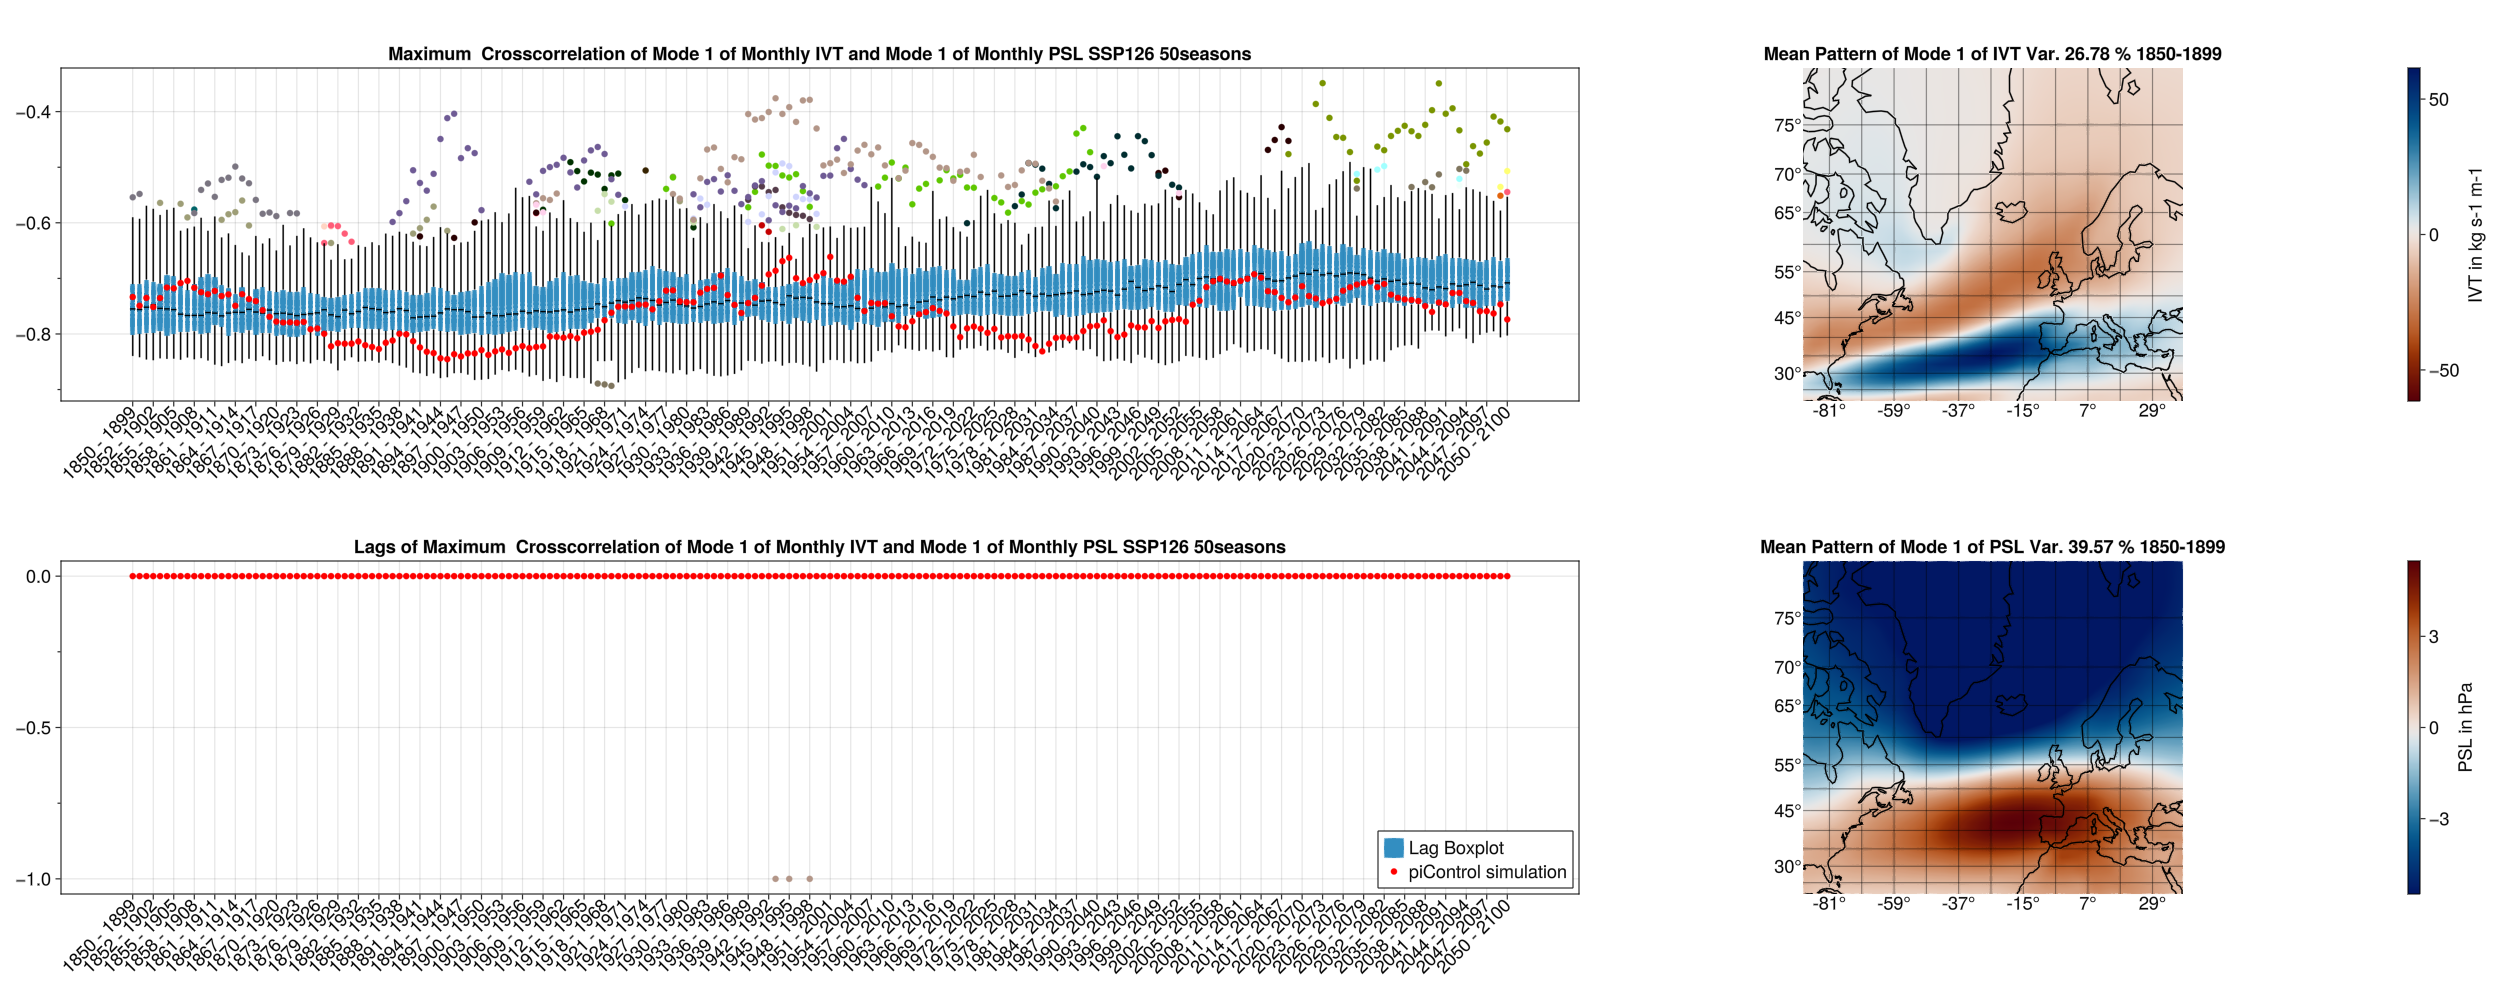
\includegraphics[width=0.95\textwidth]{figures/crosscorrelation_boxplot_ivt_psl_modes11_ssp126_50seasons.png}
    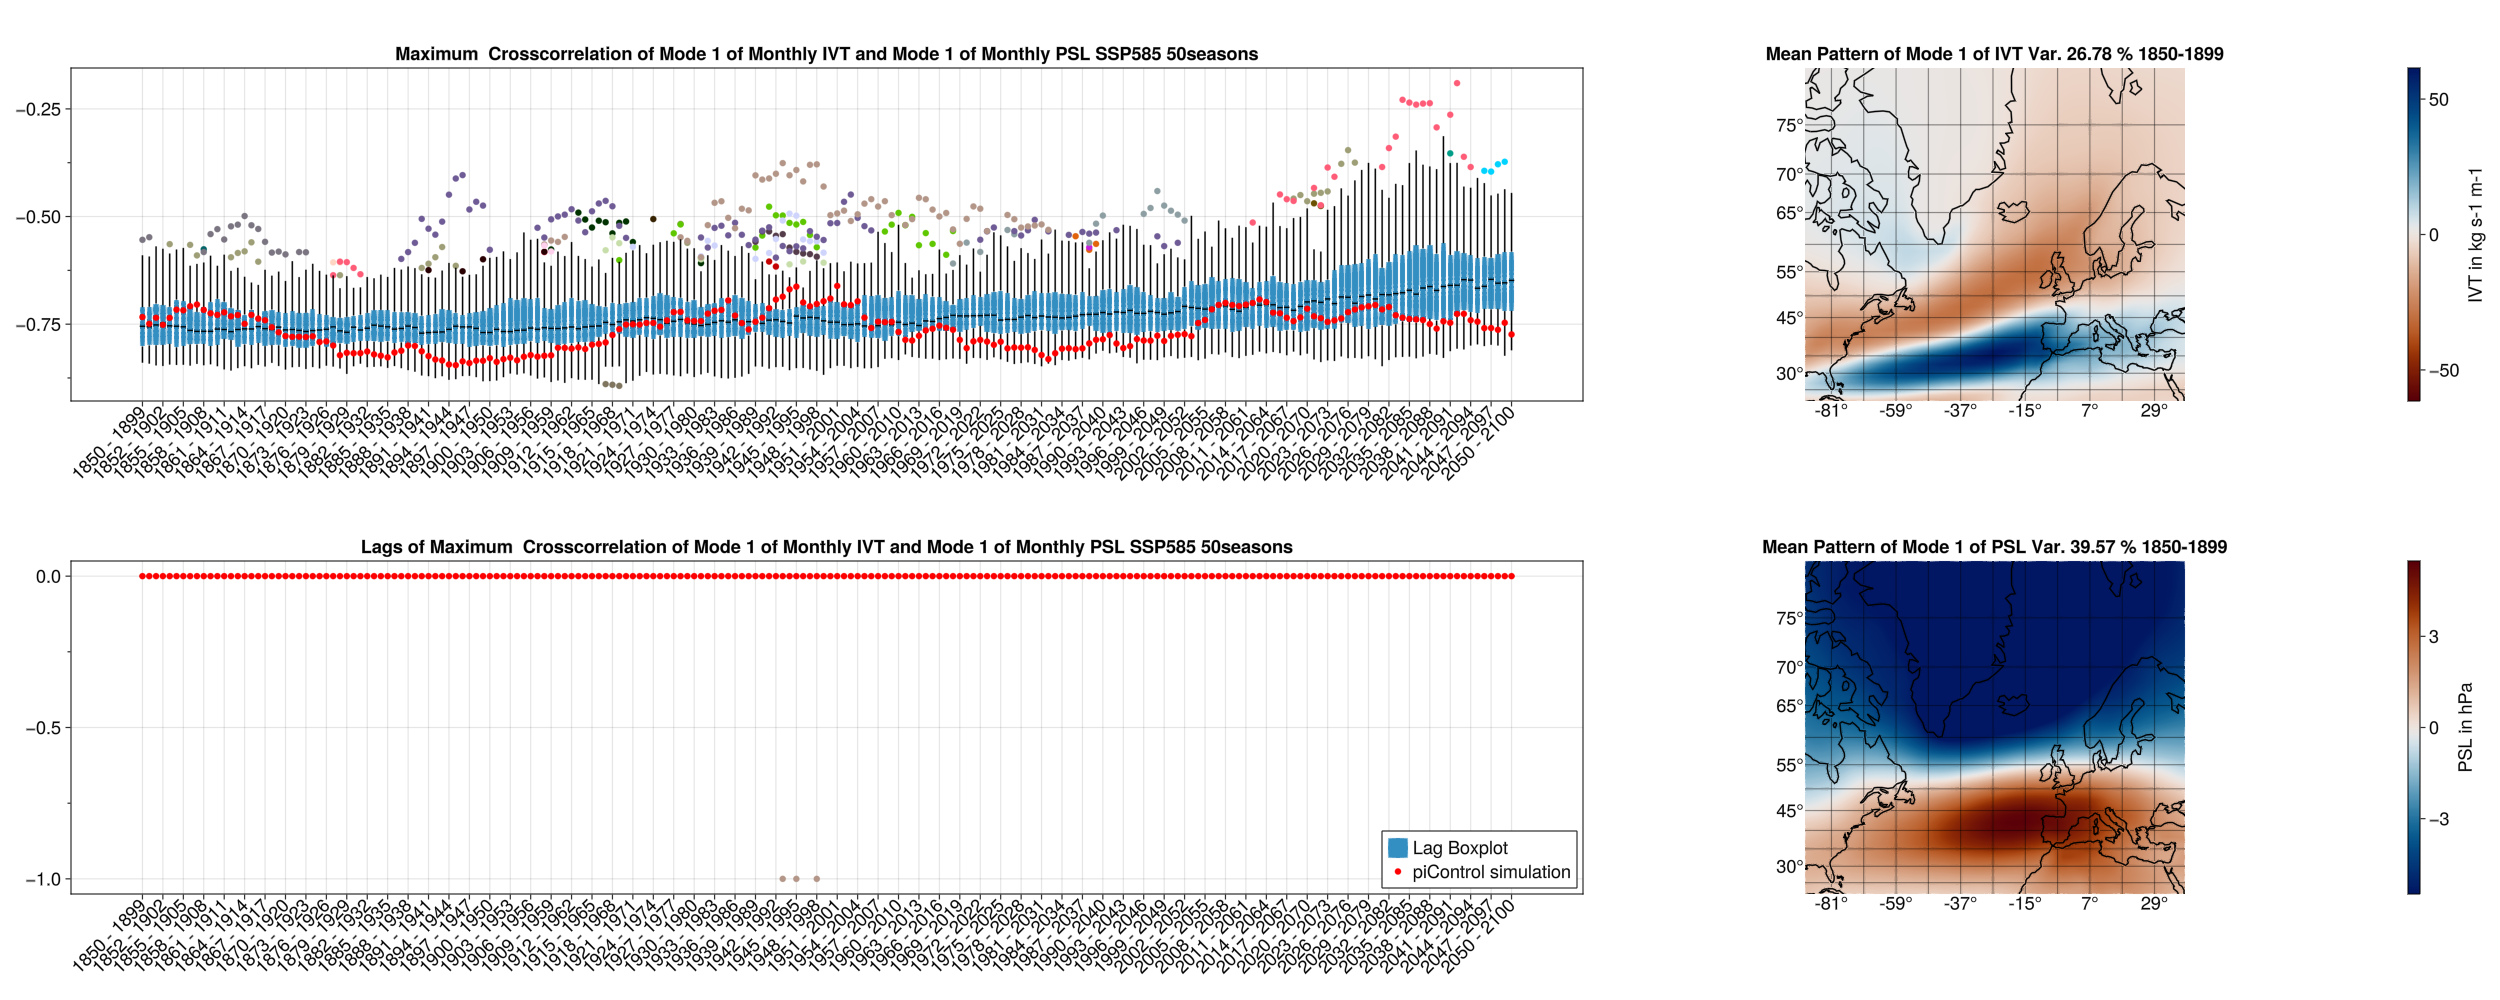
\includegraphics[width=0.95\textwidth]{figures/crosscorrelation_boxplot_ivt_psl_modes11_ssp585_50seasons.png}
  \end{center}
  \caption{Maximum cross correlation of Mode 1 of Sea Level Pressure and Mode 1 of IVT. On the right are images of the corresponding spatial patterns. Lag is a boxplot and indicates the shift in time used for finding the maximum (absolute) cross correlation.}
  \label{fig:crosscor ivt psl modes11}
\end{figure}

\begin{figure}
  \begin{center}
    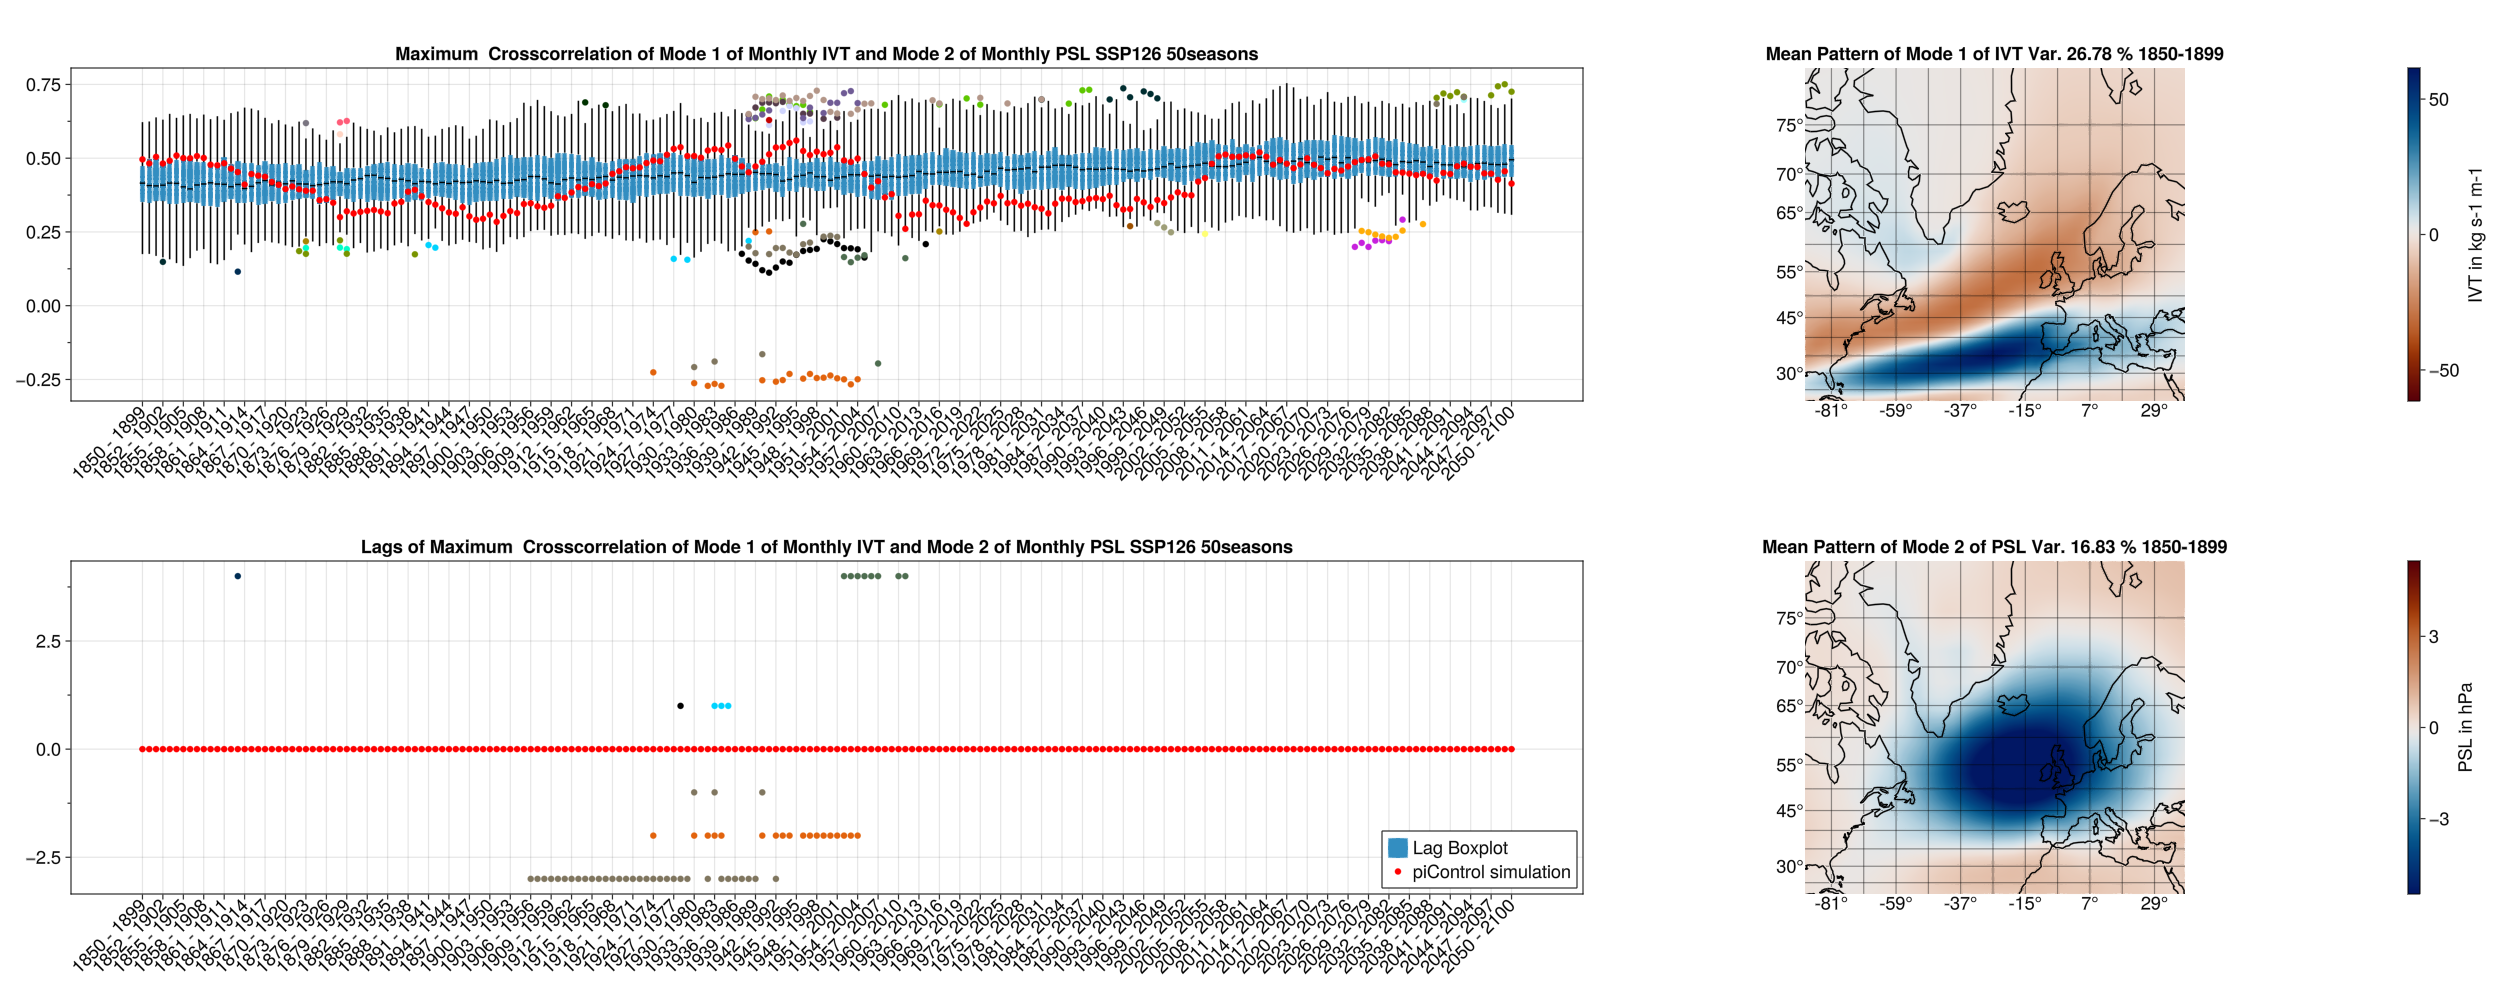
\includegraphics[width=0.95\textwidth]{figures/crosscorrelation_boxplot_ivt_psl_modes12_ssp126_50seasons.png}
    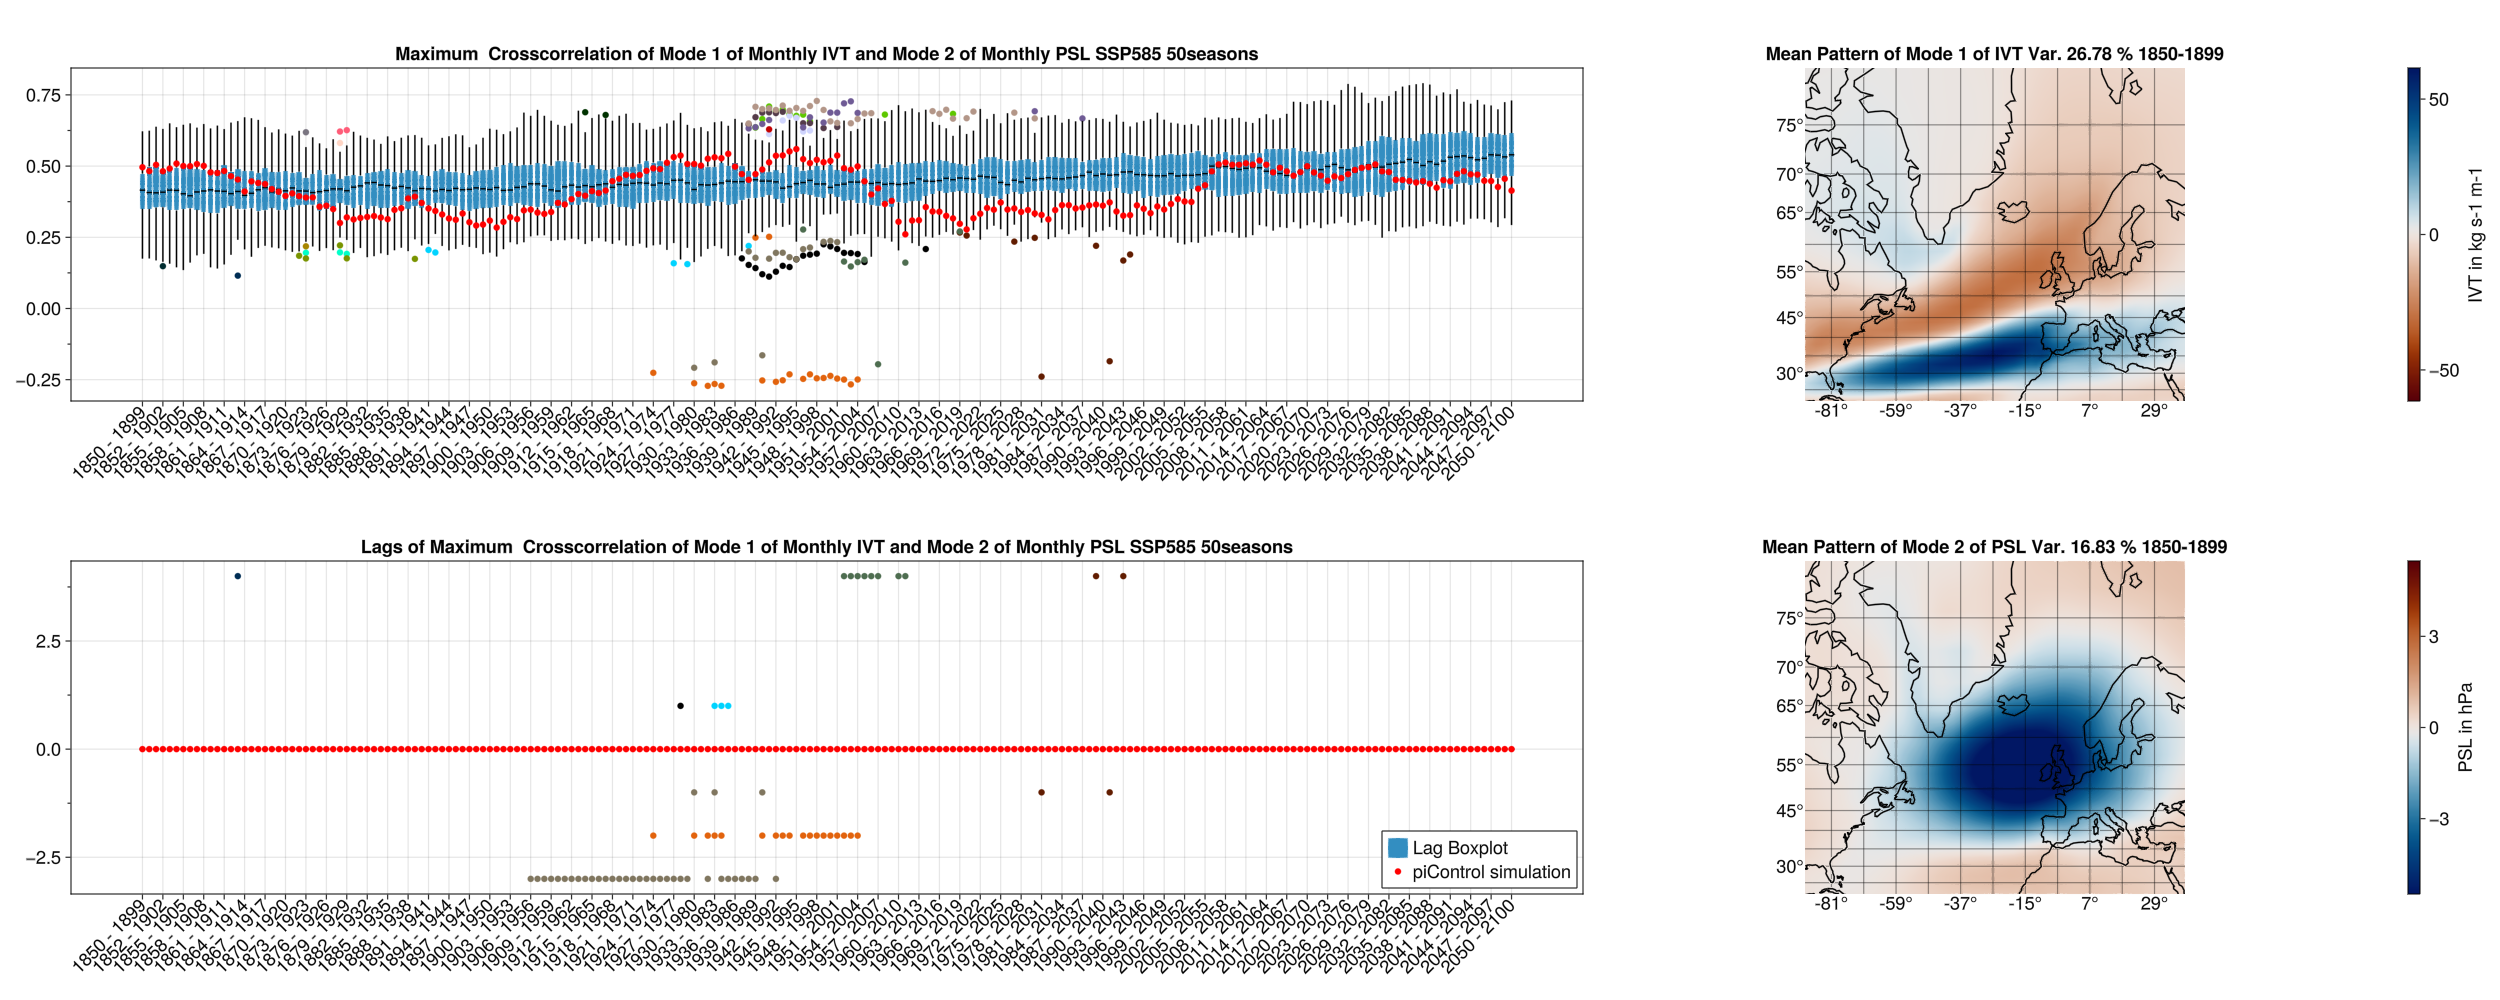
\includegraphics[width=0.95\textwidth]{figures/crosscorrelation_boxplot_ivt_psl_modes12_ssp585_50seasons.png}
  \end{center}
  \caption{Same as Figure~\ref{fig:crosscor ivt psl modes11}, but with mode 2 of Sea Level Pressure (EAP).}
  \label{fig:crosscor ivt psl modes12}
\end{figure}

\begin{figure}
  \begin{center}
    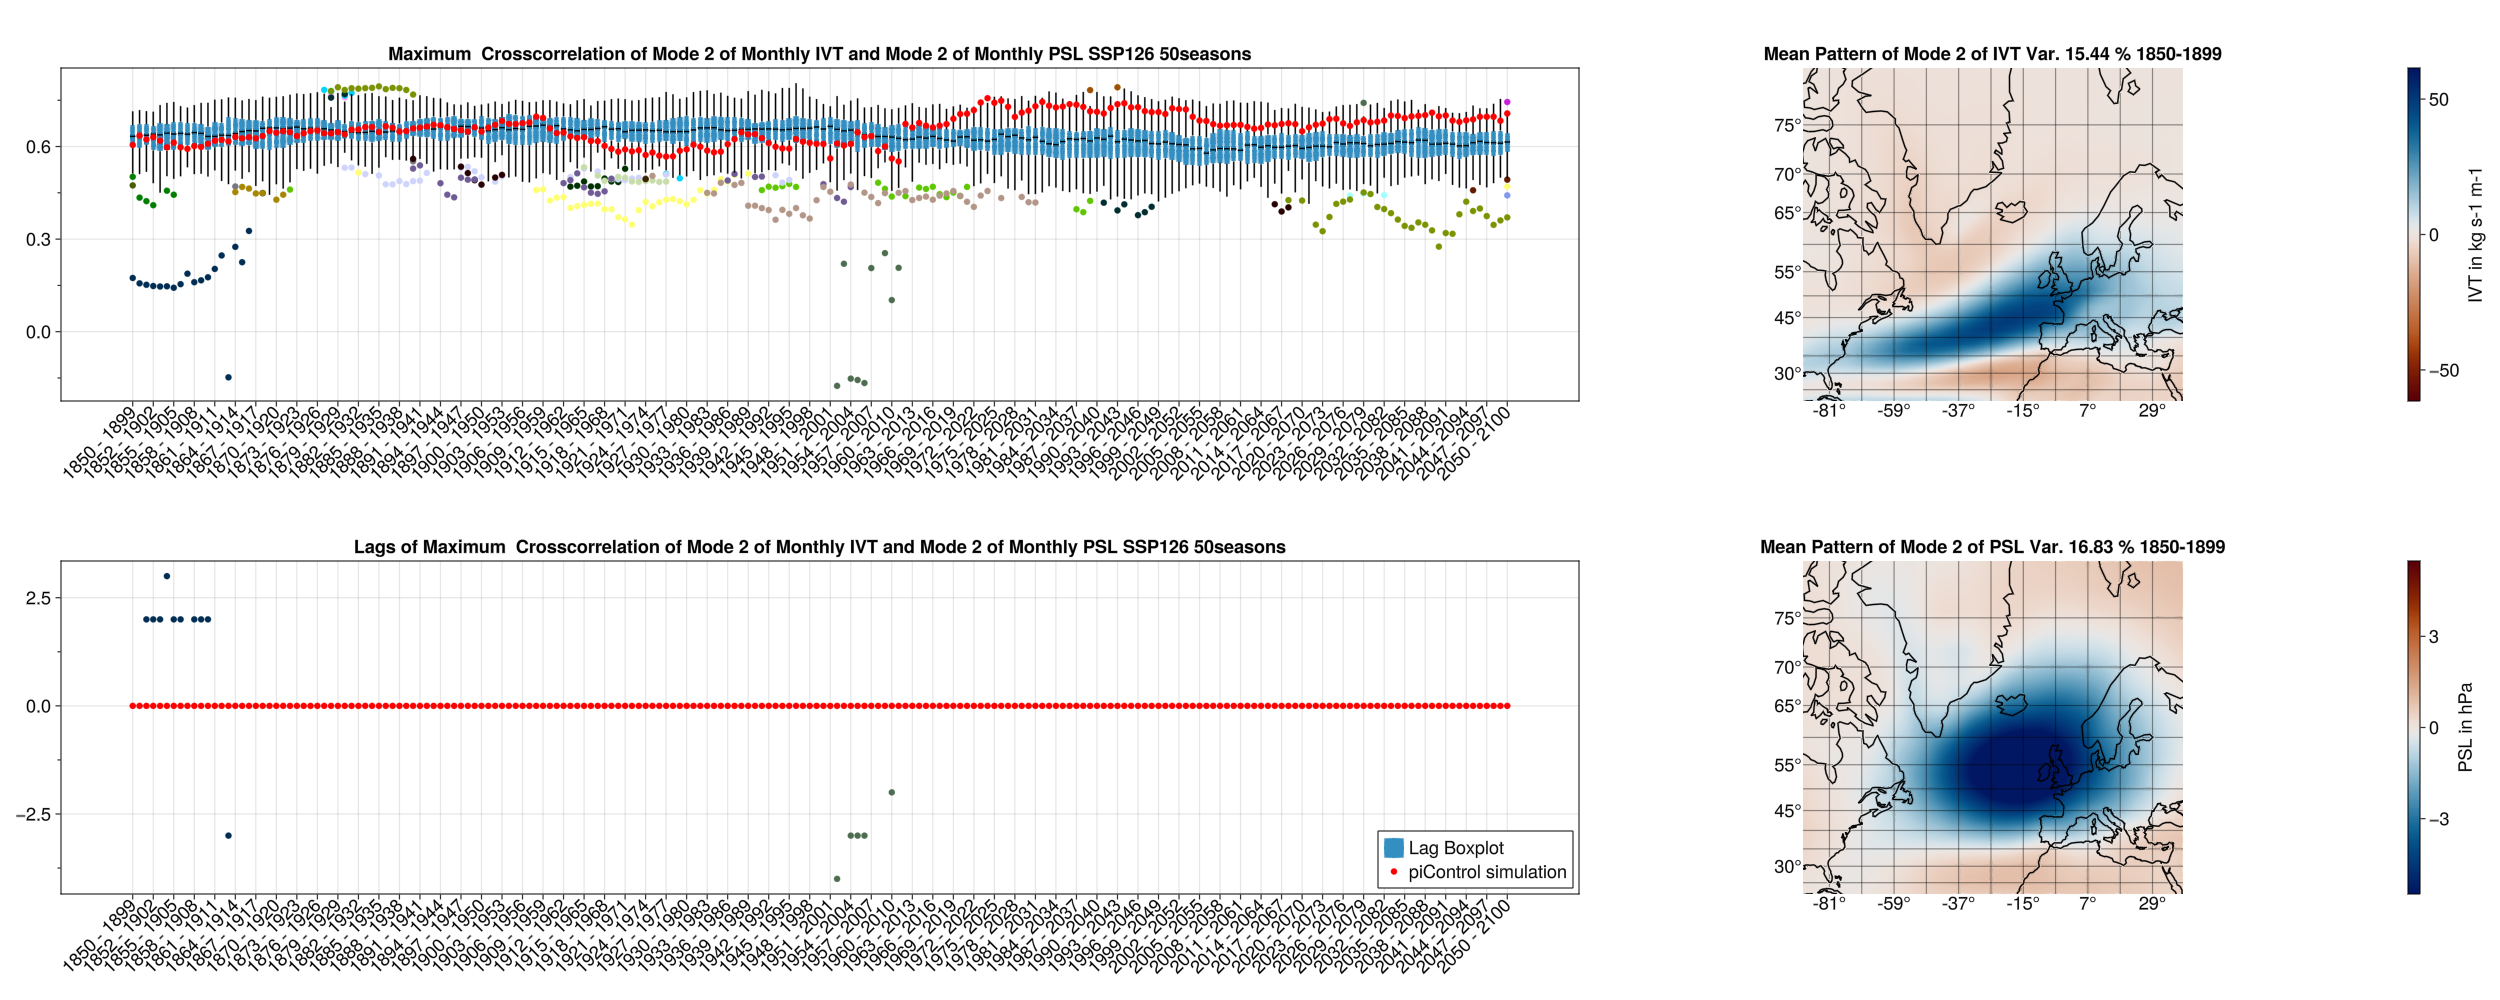
\includegraphics[width=0.95\textwidth]{figures/crosscorrelation_boxplot_ivt_psl_modes22_ssp126_50seasons.png}
    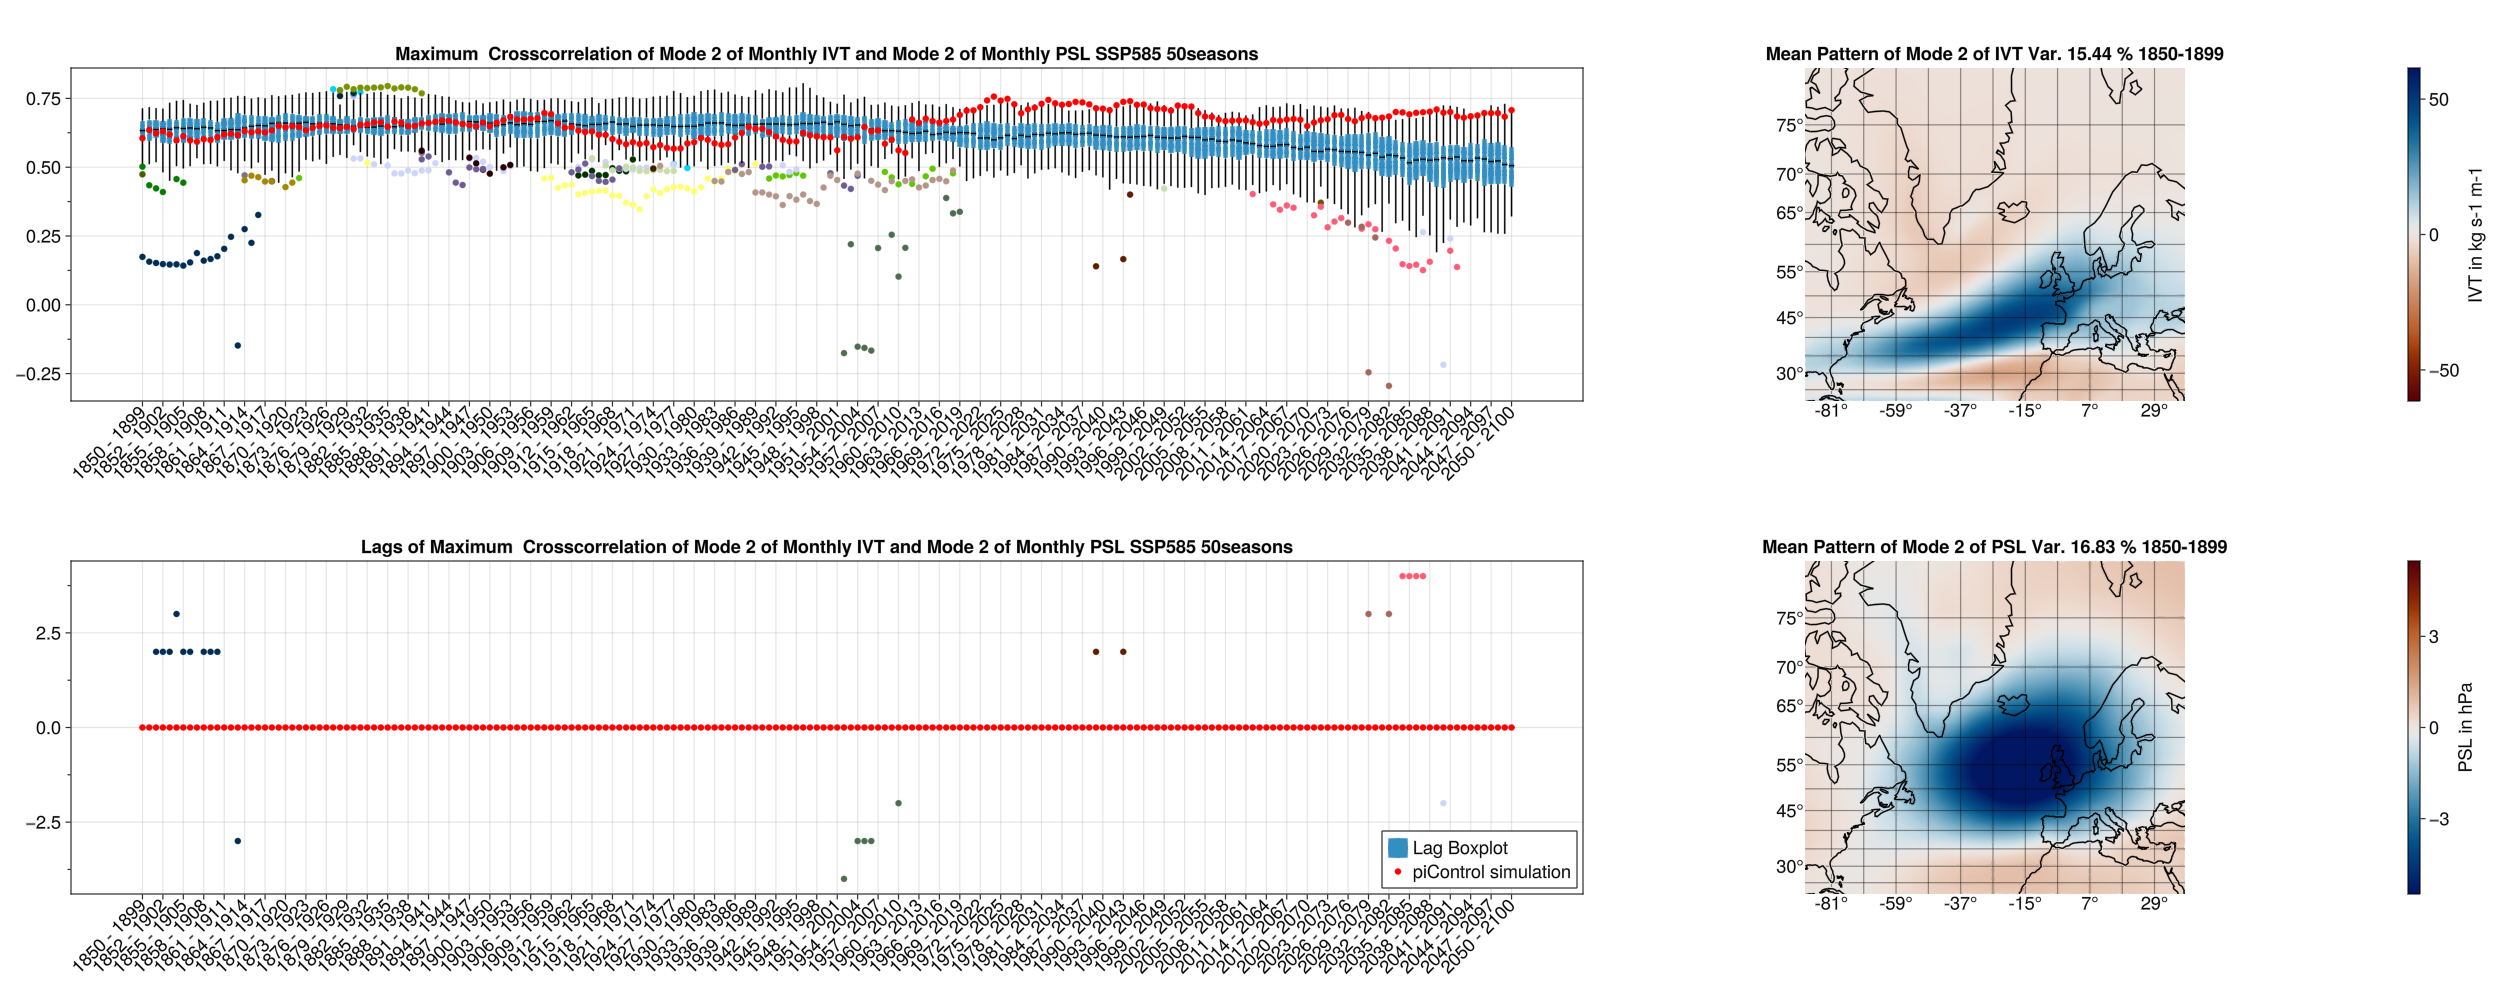
\includegraphics[width=0.95\textwidth]{figures/crosscorrelation_boxplot_ivt_psl_modes22_ssp585_50seasons.png}
  \end{center}
  \caption{Same as Figure~\ref{fig:crosscor ivt psl modes11}, but with mode 2 of Sea Level Pressure (EAP) and IVT.}
  \label{fig:crosscor ivt psl modes22}
\end{figure}


\begin{figure}
  \begin{center}
    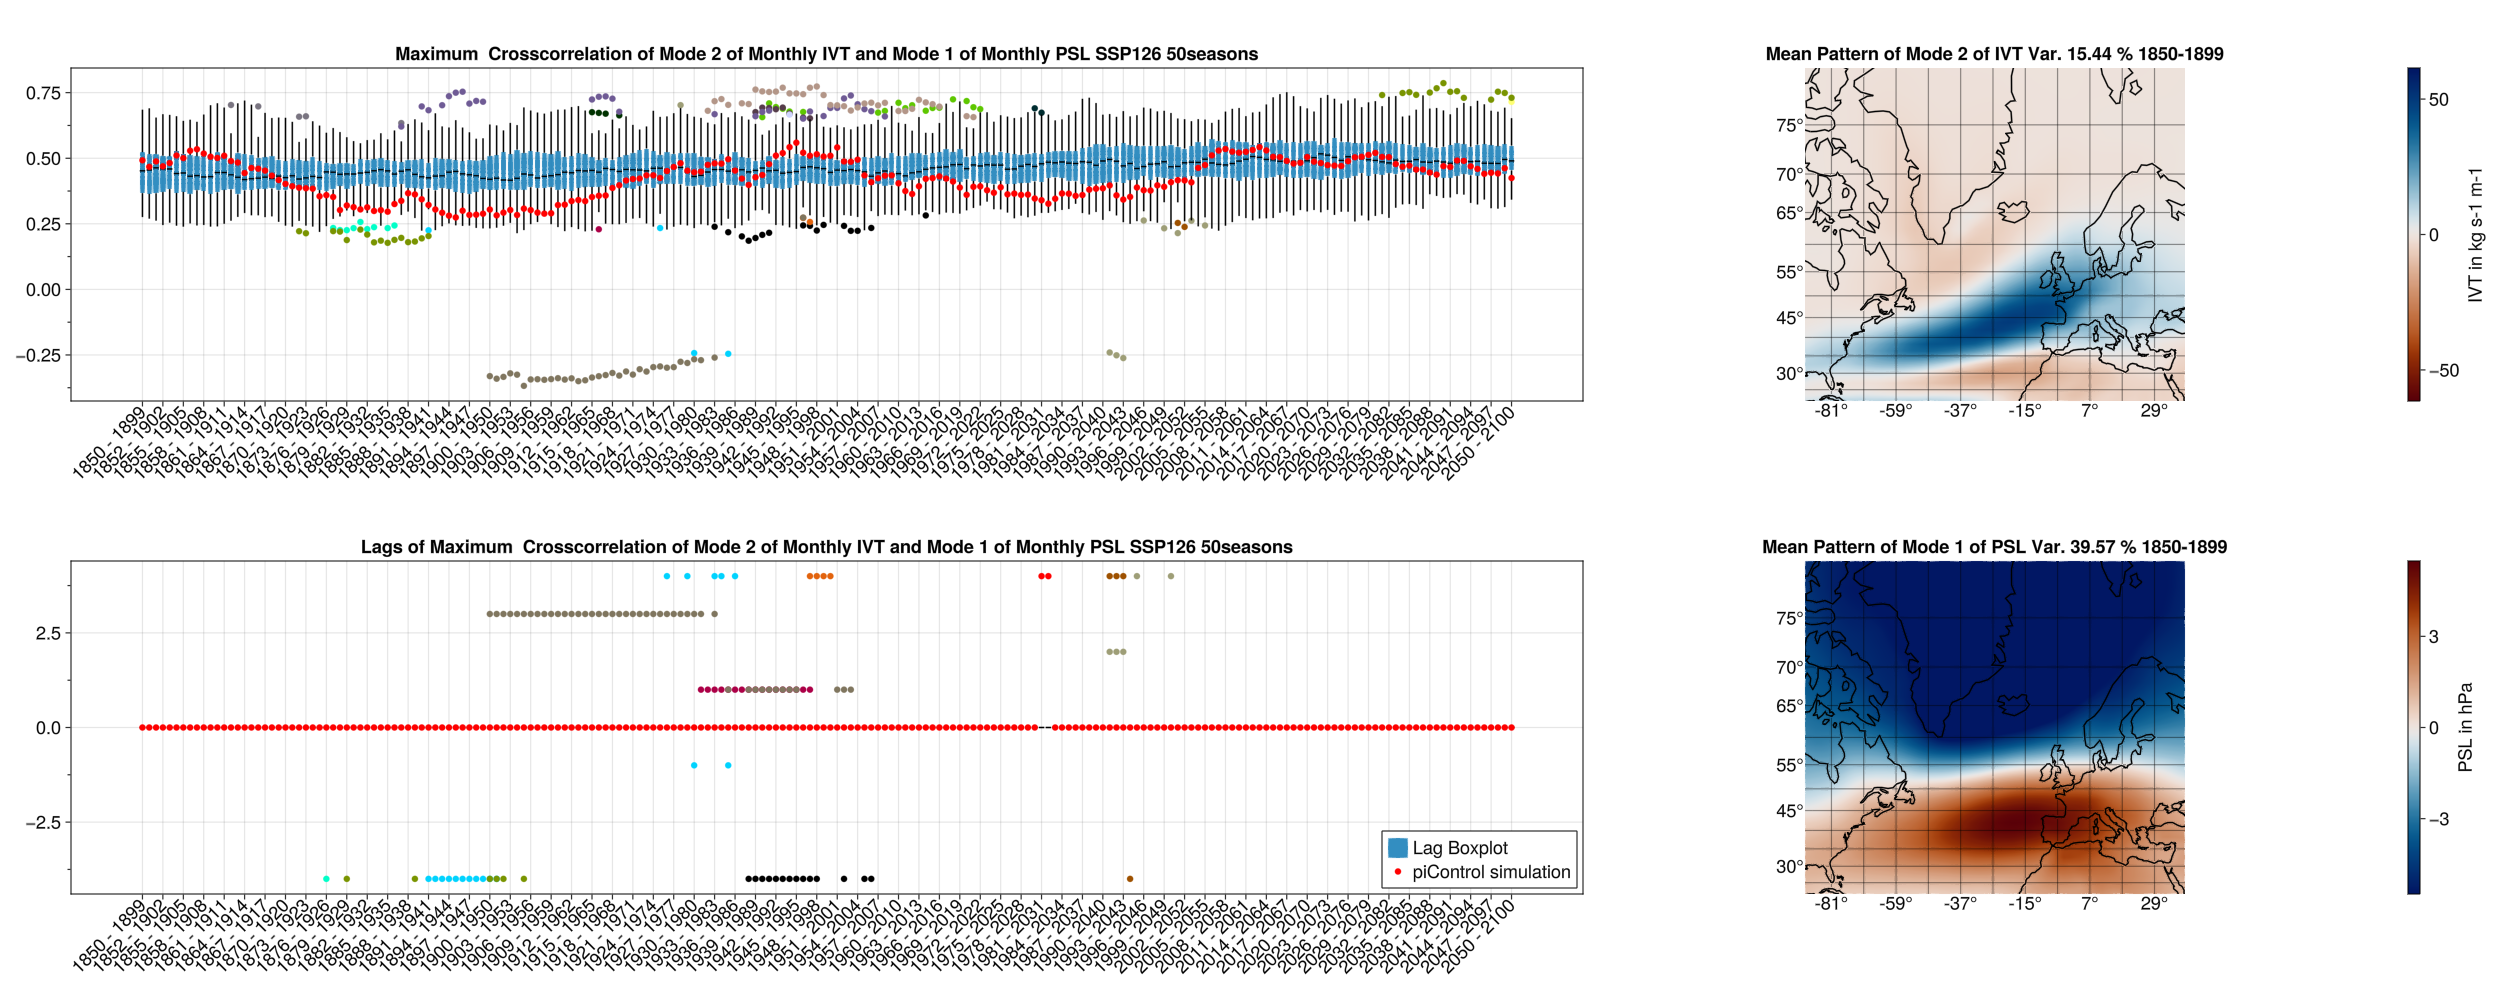
\includegraphics[width=0.95\textwidth]{figures/crosscorrelation_boxplot_ivt_psl_modes21_ssp126_50seasons.png}
    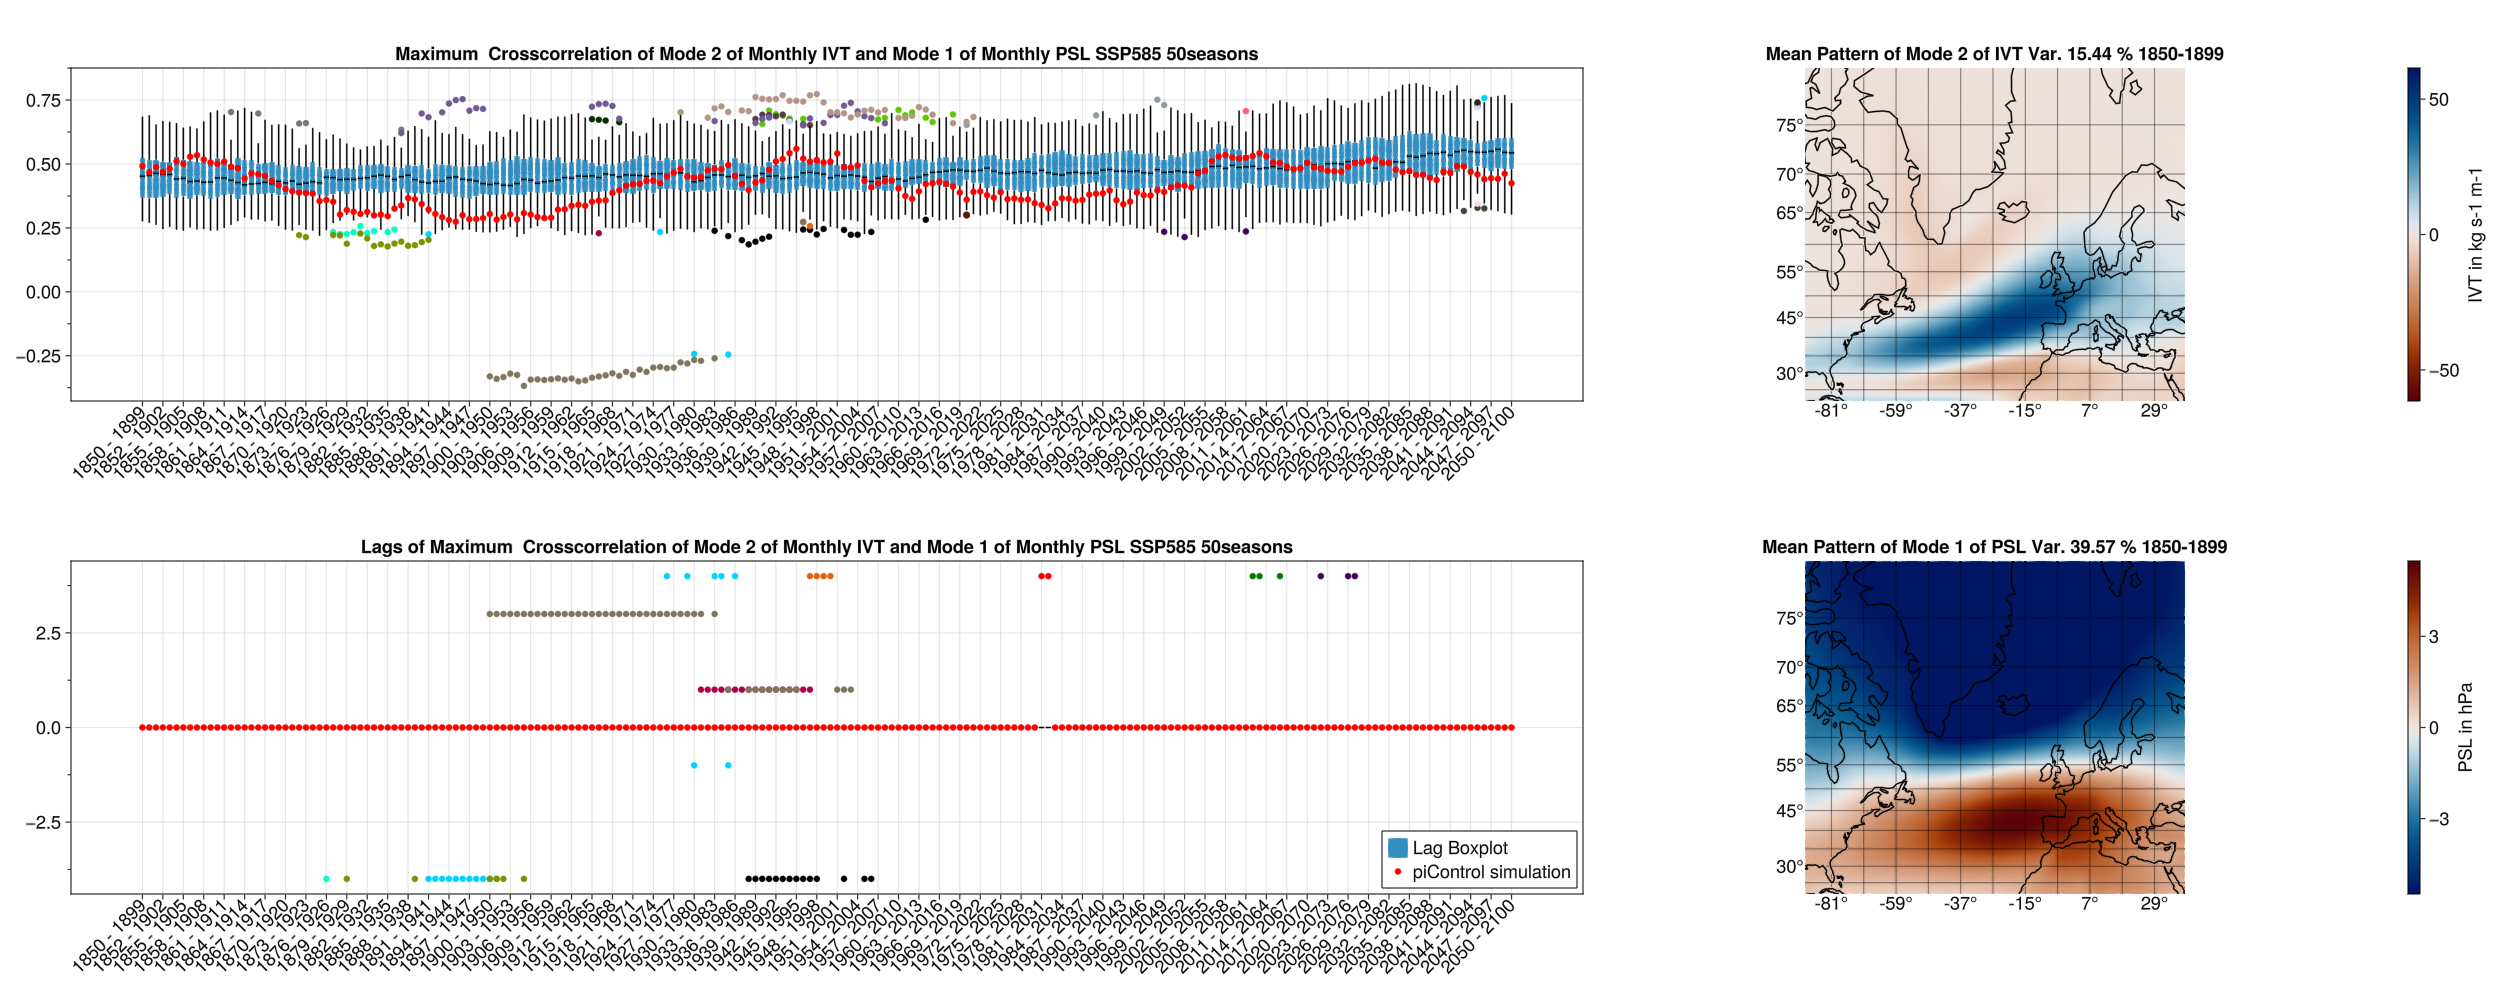
\includegraphics[width=0.95\textwidth]{figures/crosscorrelation_boxplot_ivt_psl_modes21_ssp585_50seasons.png}
  \end{center}
  \caption{Same as Figure~\ref{fig:crosscor ivt psl modes11}, but with mode 2 of IVT EOF.}
  \label{fig:crosscor ivt psl modes21}
\end{figure}






\subsubsection{Relationships of Precipitation and IVT EOFs}

\begin{figure}
  \begin{center}
    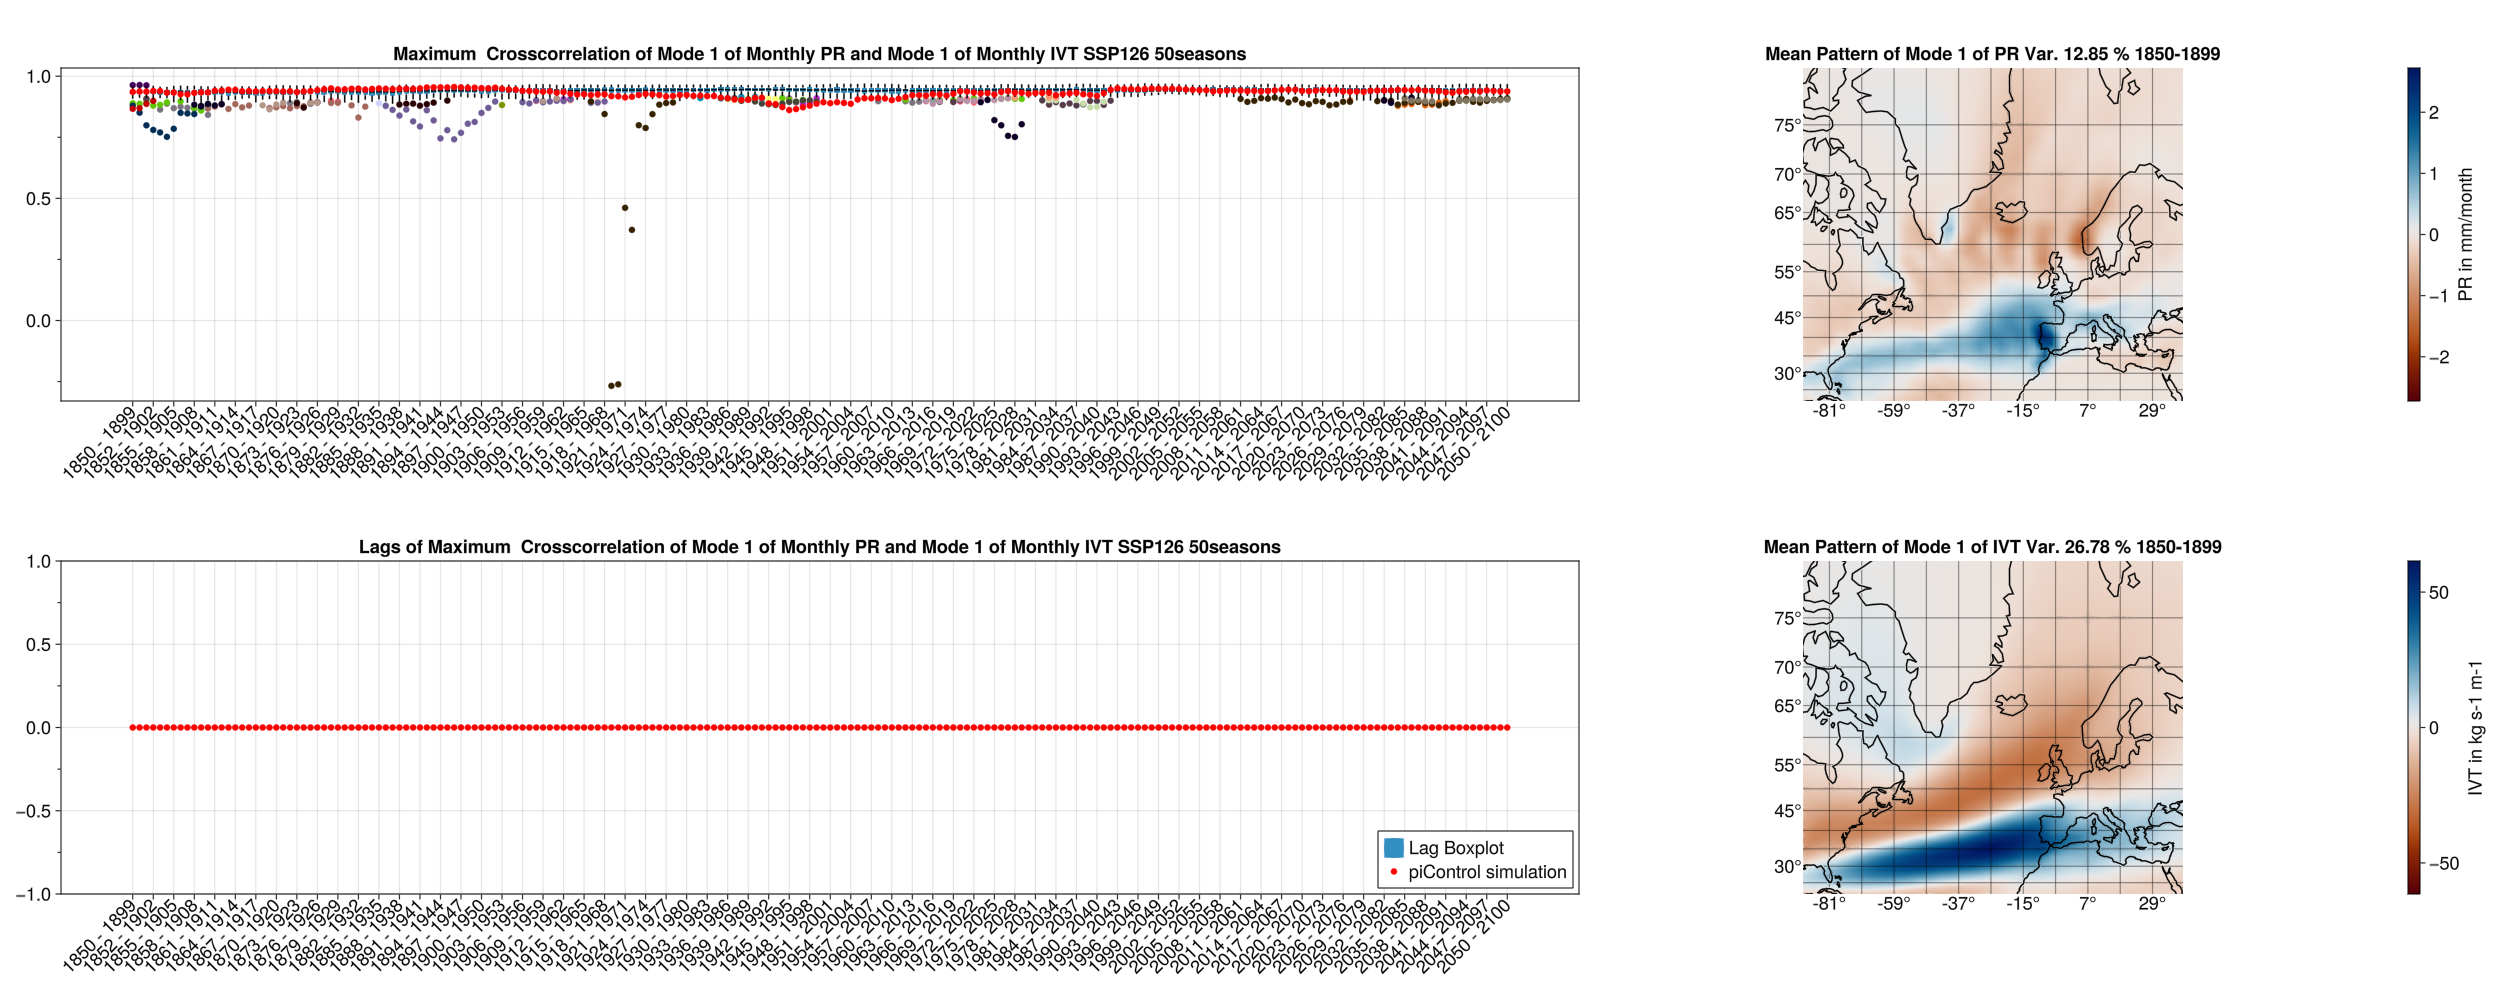
\includegraphics[width=0.95\textwidth]{figures/crosscorrelation_boxplot_pr_ivt_modes11_ssp126_50seasons.png}
    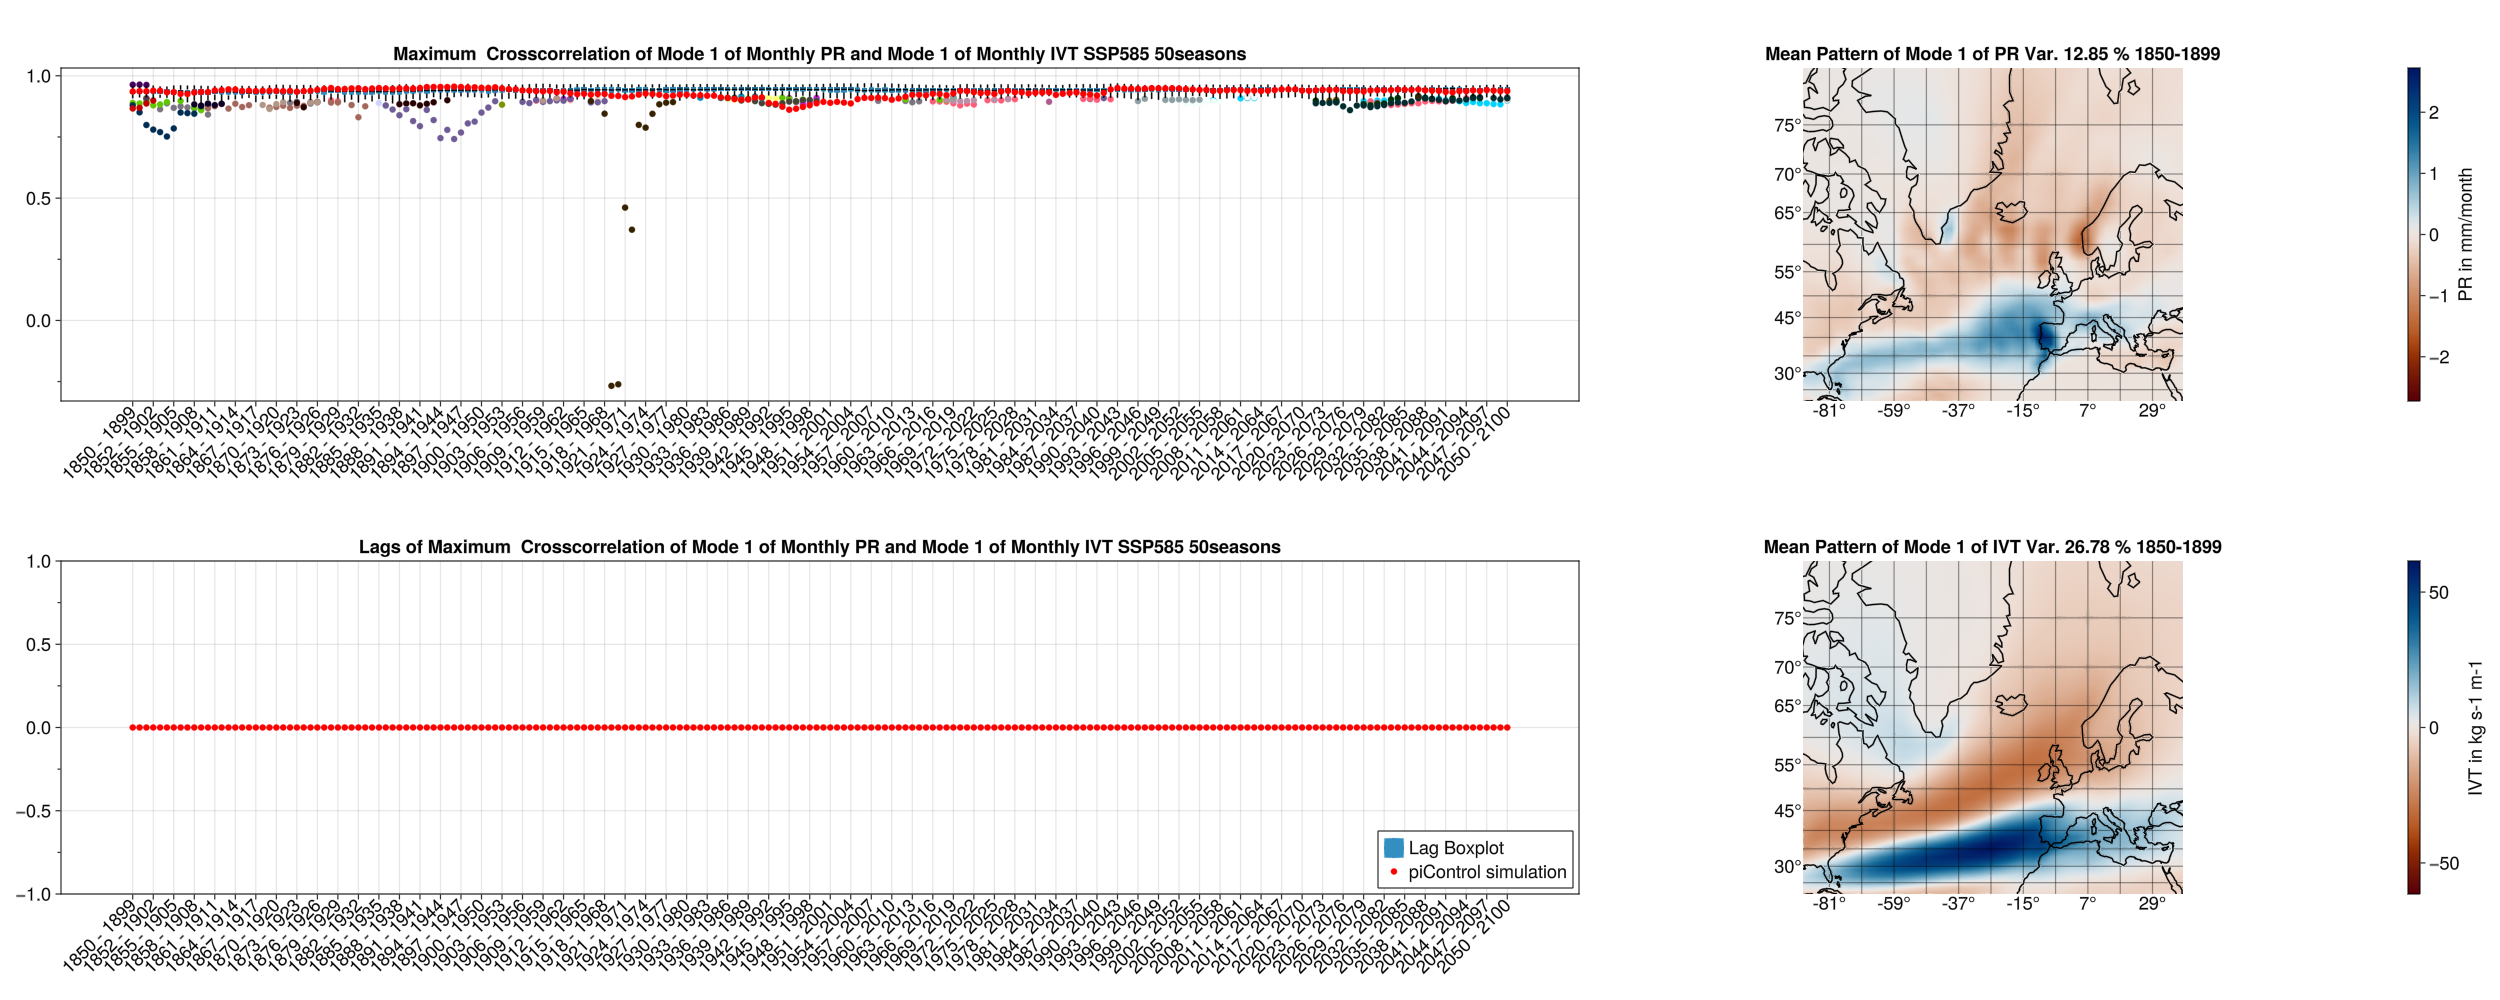
\includegraphics[width=0.95\textwidth]{figures/crosscorrelation_boxplot_pr_ivt_modes11_ssp585_50seasons.png}
  \end{center}
  \caption{Same as Figure~\ref{fig:crosscor ivt psl modes11}, but with modes 1 of precipitation and IVT EOFs.}\label{fig:crosscor pr ivt modes11}
\end{figure}

\begin{figure}
  \begin{center}
    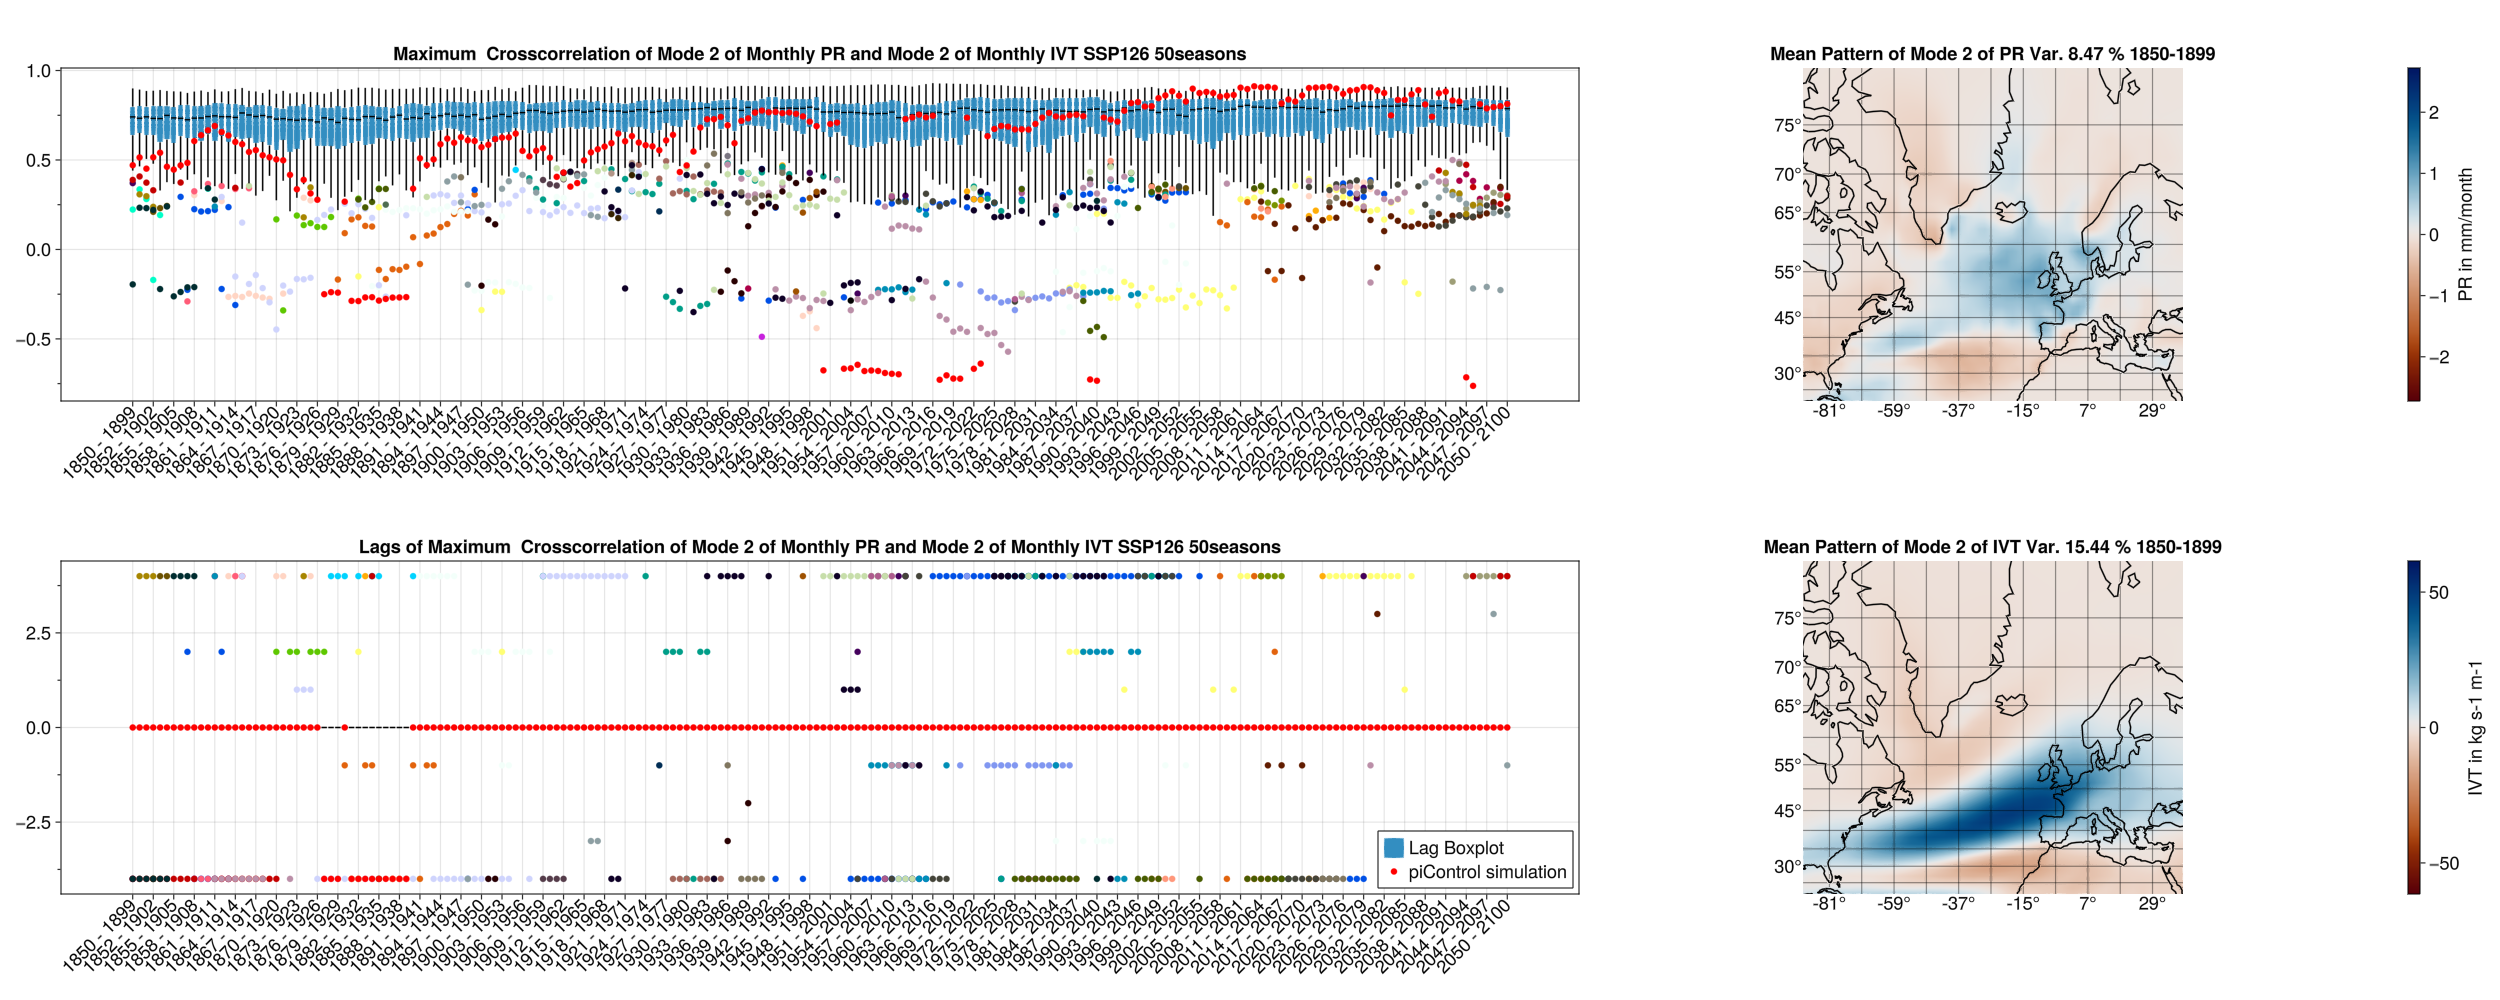
\includegraphics[width=0.95\textwidth]{figures/crosscorrelation_boxplot_pr_ivt_modes22_ssp126_50seasons.png}
    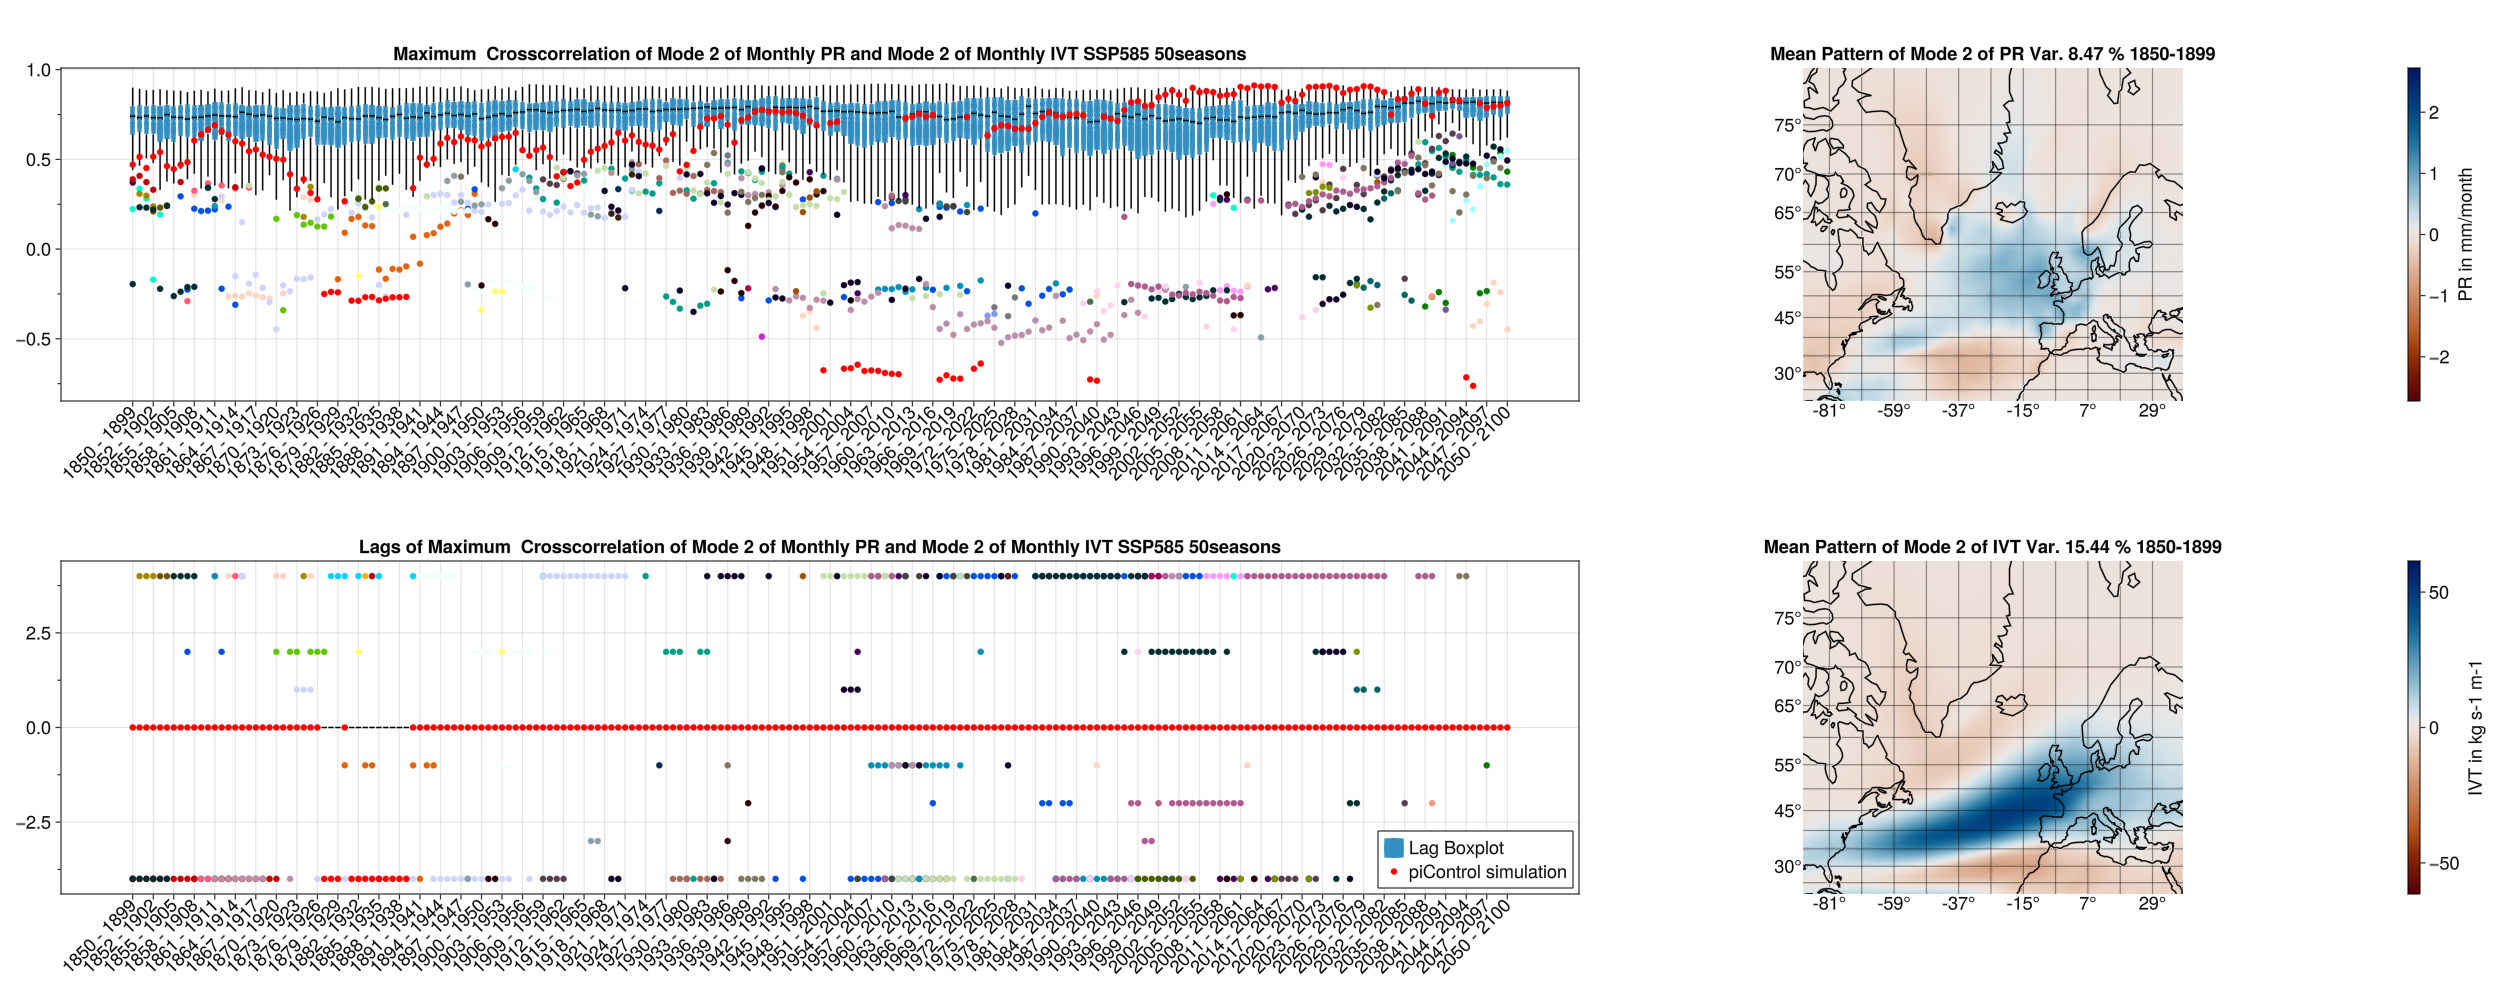
\includegraphics[width=0.95\textwidth]{figures/crosscorrelation_boxplot_pr_ivt_modes22_ssp585_50seasons.png}
  \end{center}
  \caption{Same as Figure~\ref{fig:crosscor pr ivt modes11}, but with modes 2 of each variables' EOFs.}\label{fig:crosscor pr ivt modes22}
\end{figure}


\subsubsection{Relationships of Precipitation and Sea Level Pressure EOFs}



\begin{figure}
  \begin{center}
    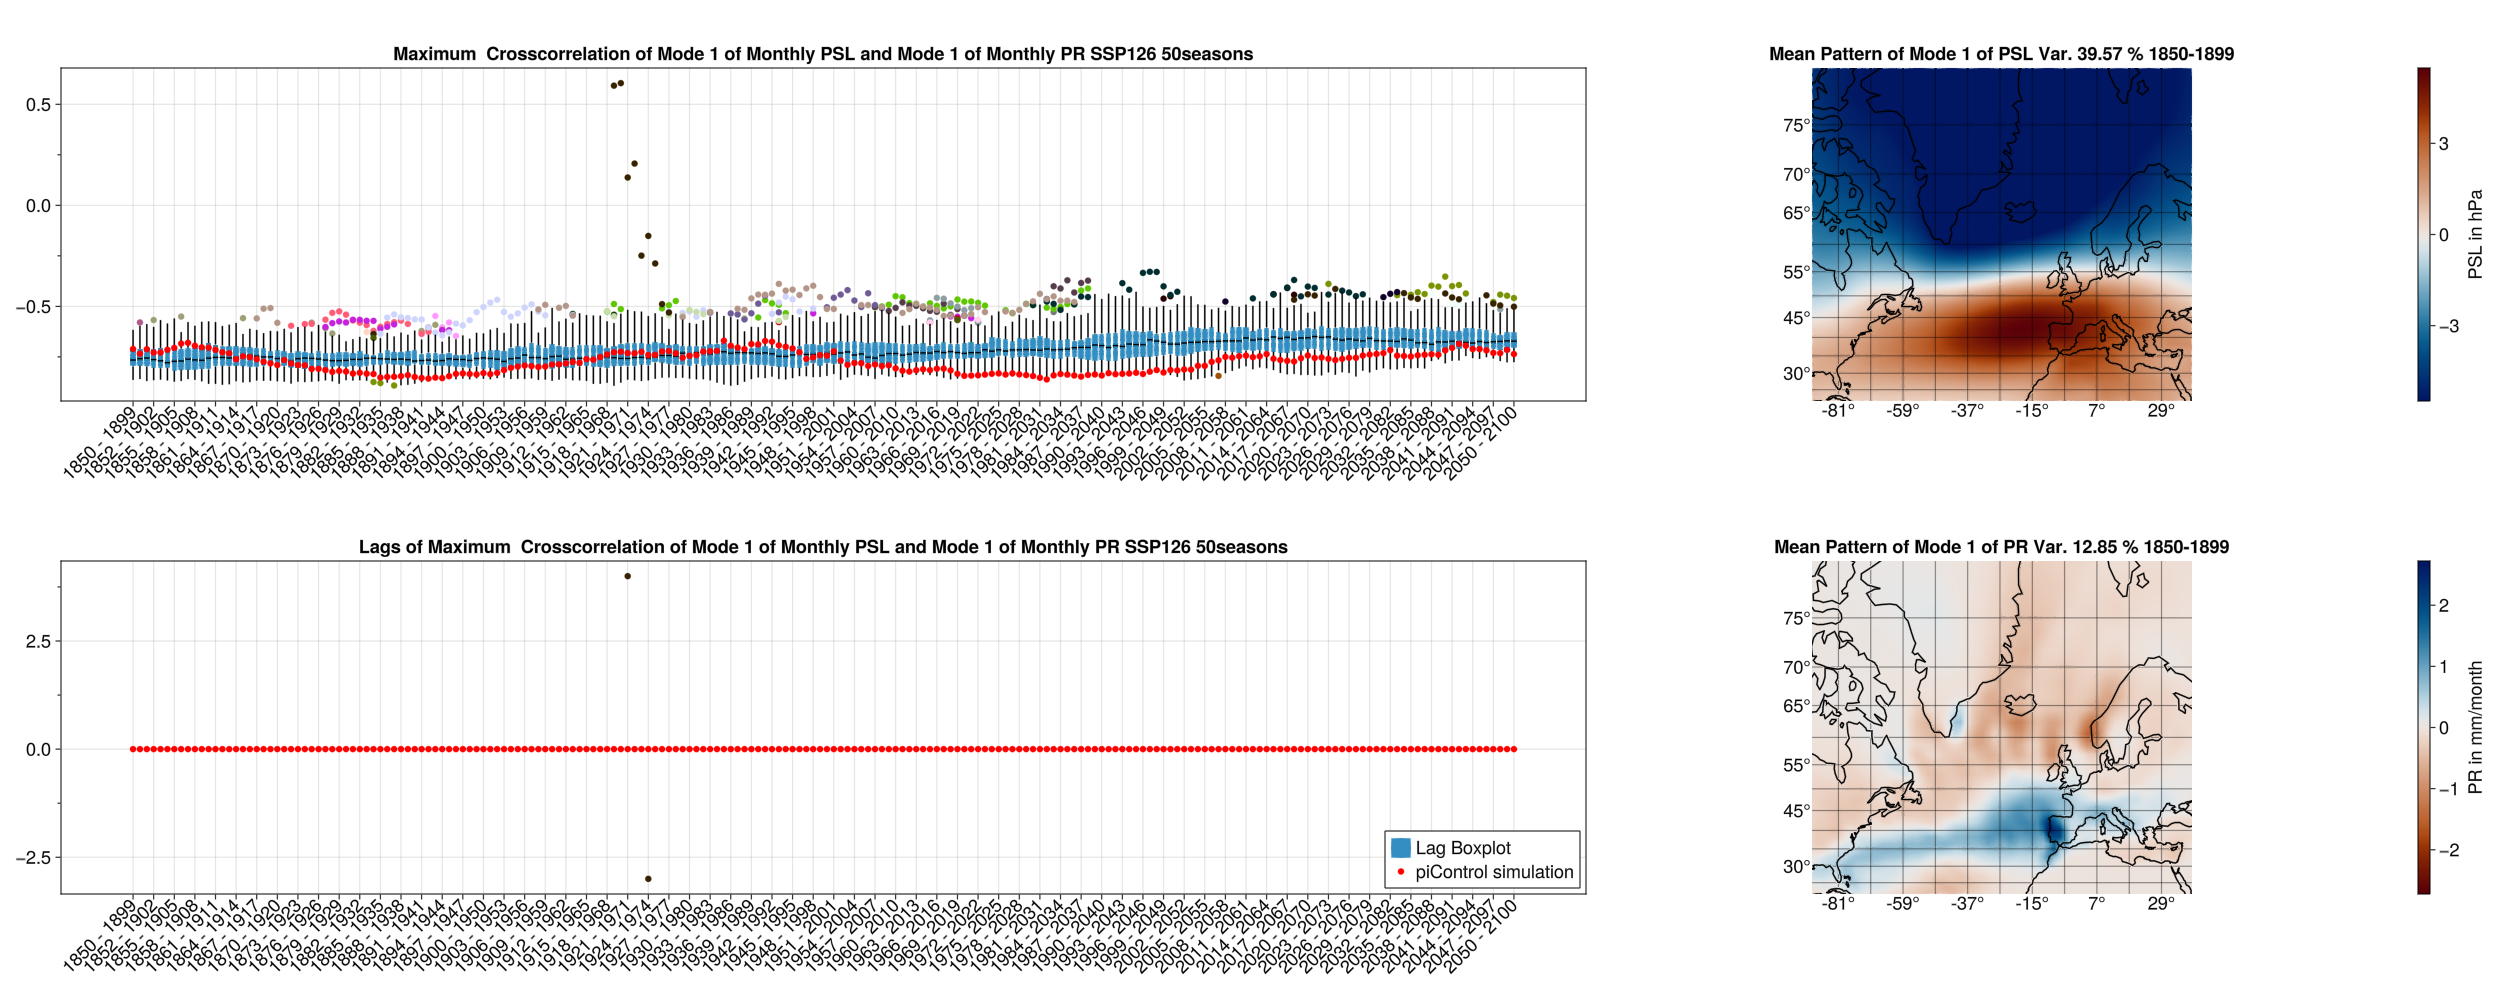
\includegraphics[width=0.95\textwidth]{figures/crosscorrelation_boxplot_psl_pr_modes11_ssp126_50seasons.png}
    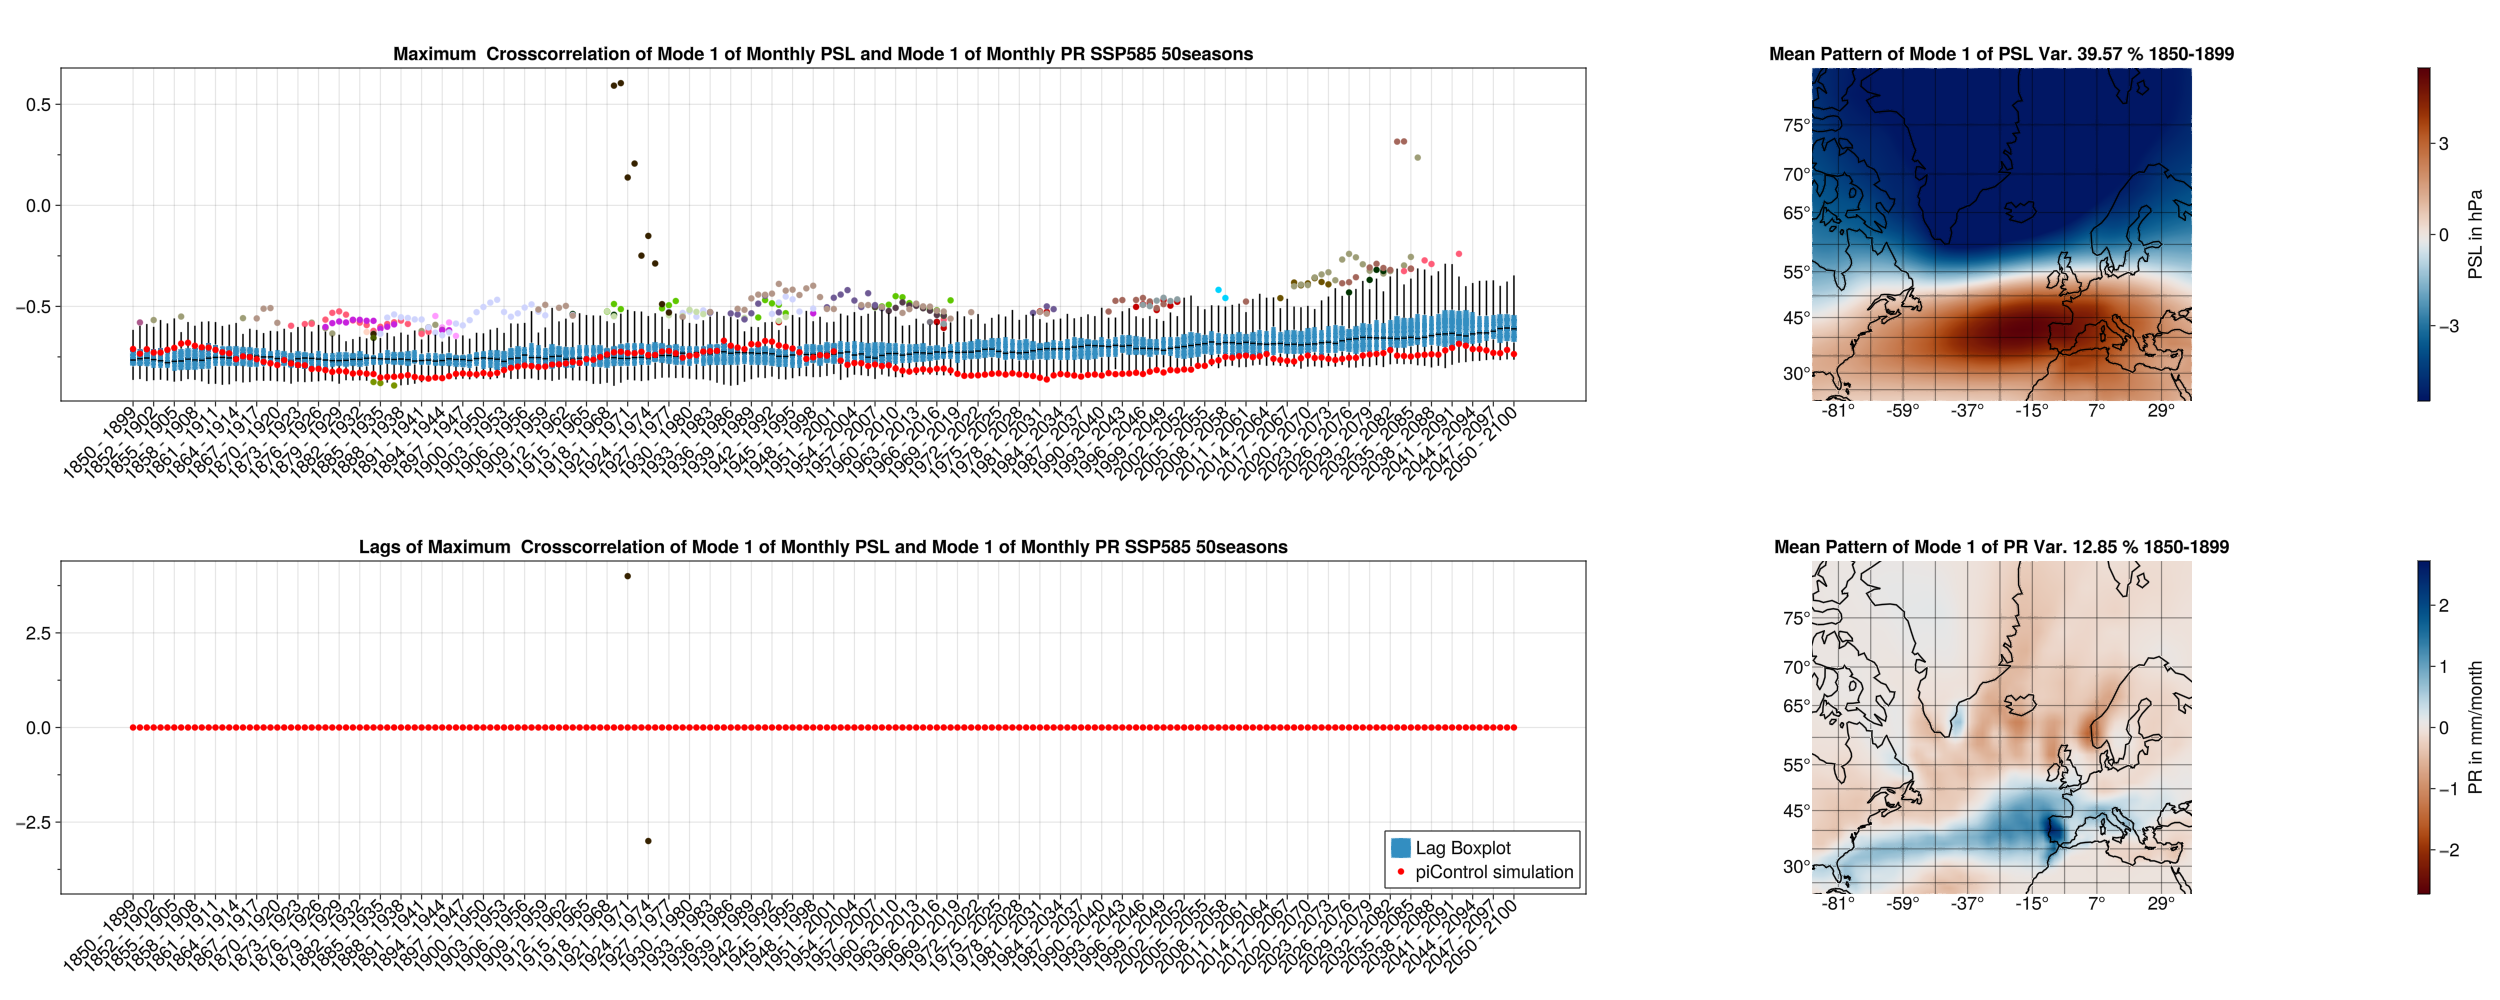
\includegraphics[width=0.95\textwidth]{figures/crosscorrelation_boxplot_psl_pr_modes11_ssp585_50seasons.png}
  \end{center}
  \caption{Same as Figure~\ref{fig:crosscor ivt psl modes11}, but with Sea Level Pressure and precipitation EOFs.}\label{fig:crosscor psl pr modes11}
\end{figure}

\begin{figure}
  \begin{center}
    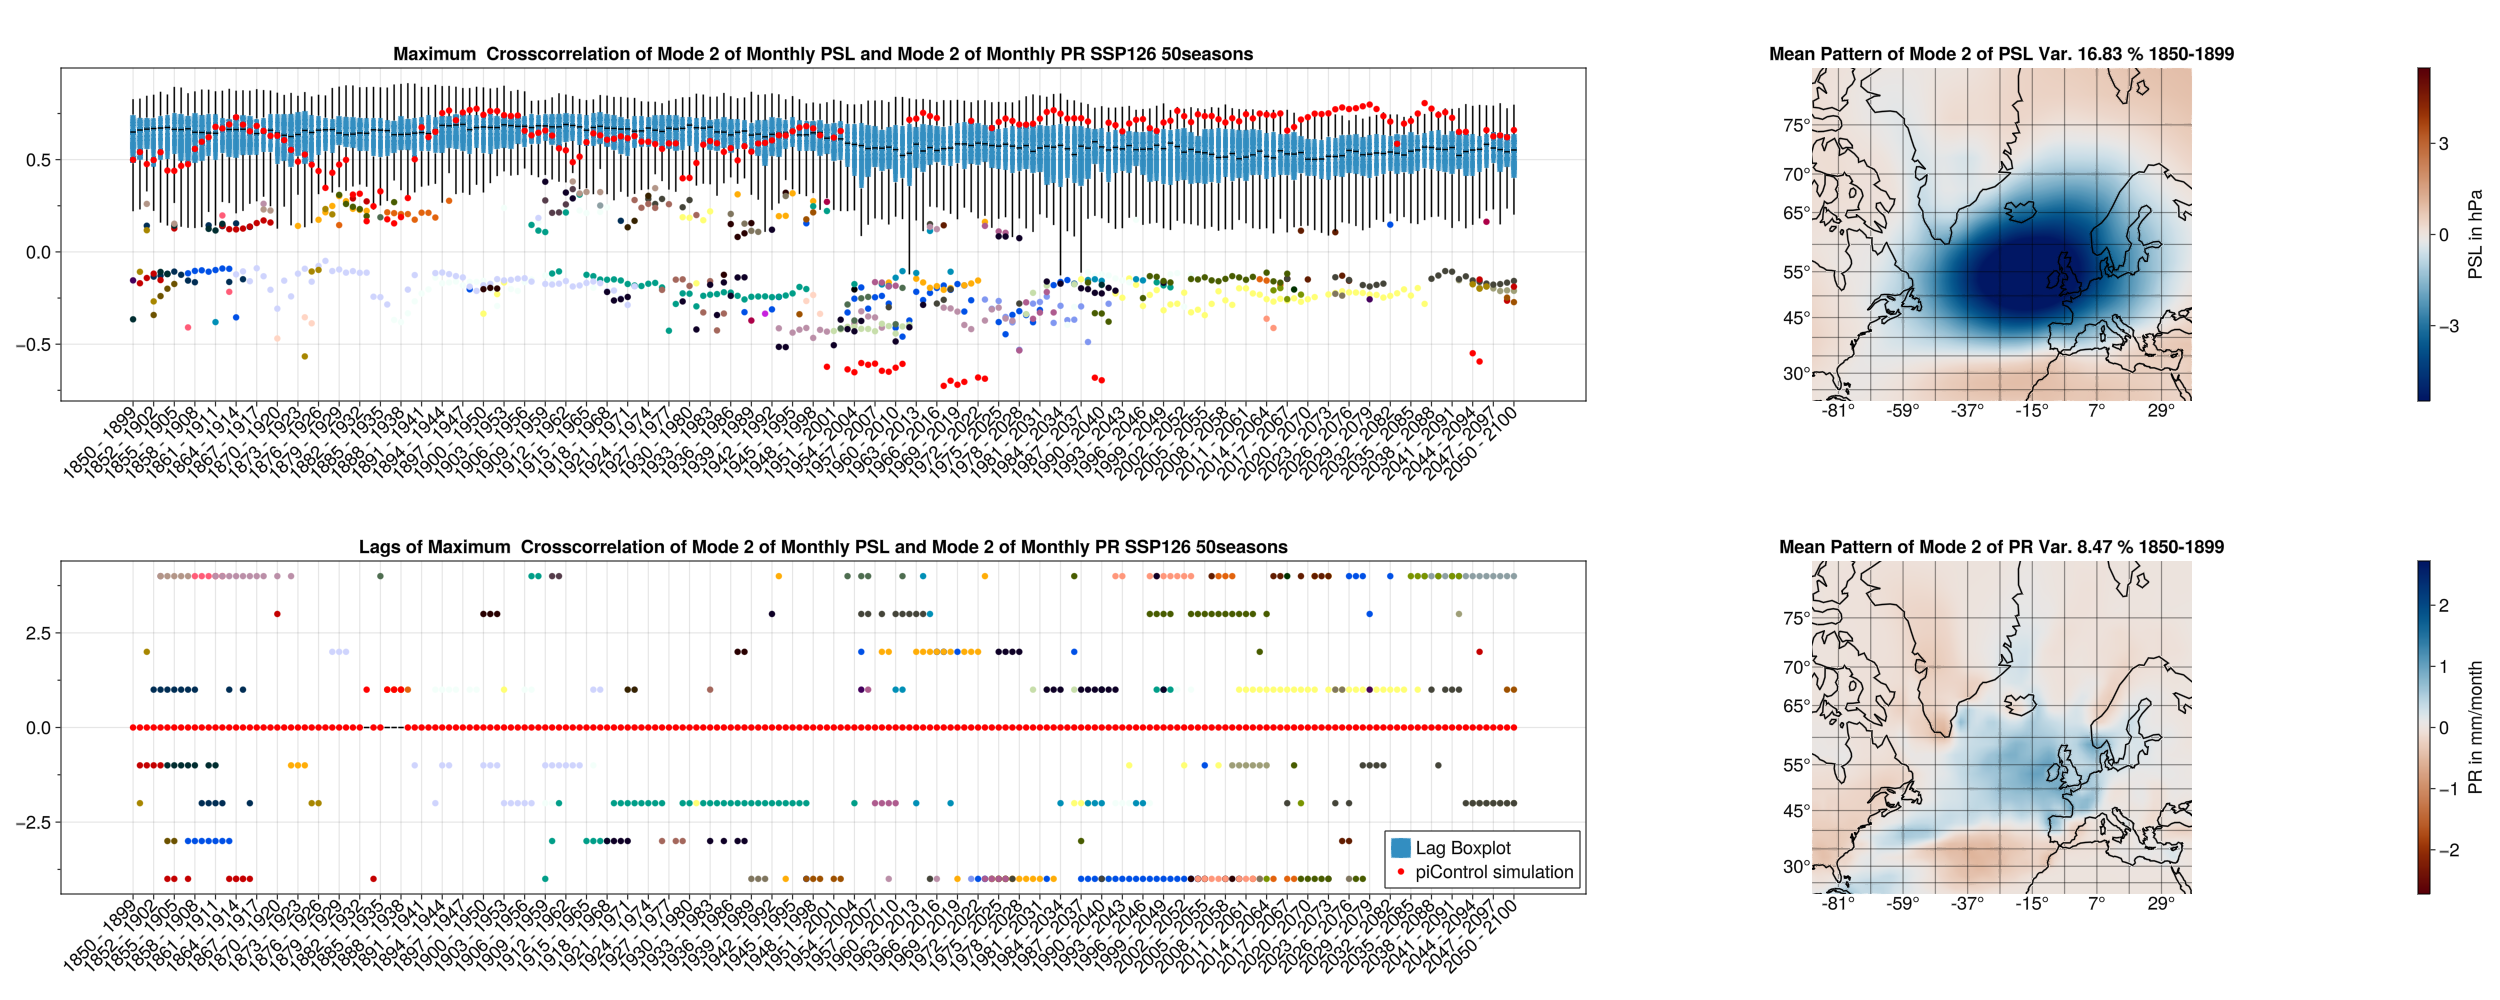
\includegraphics[width=0.95\textwidth]{figures/crosscorrelation_boxplot_psl_pr_modes22_ssp126_50seasons.png}
    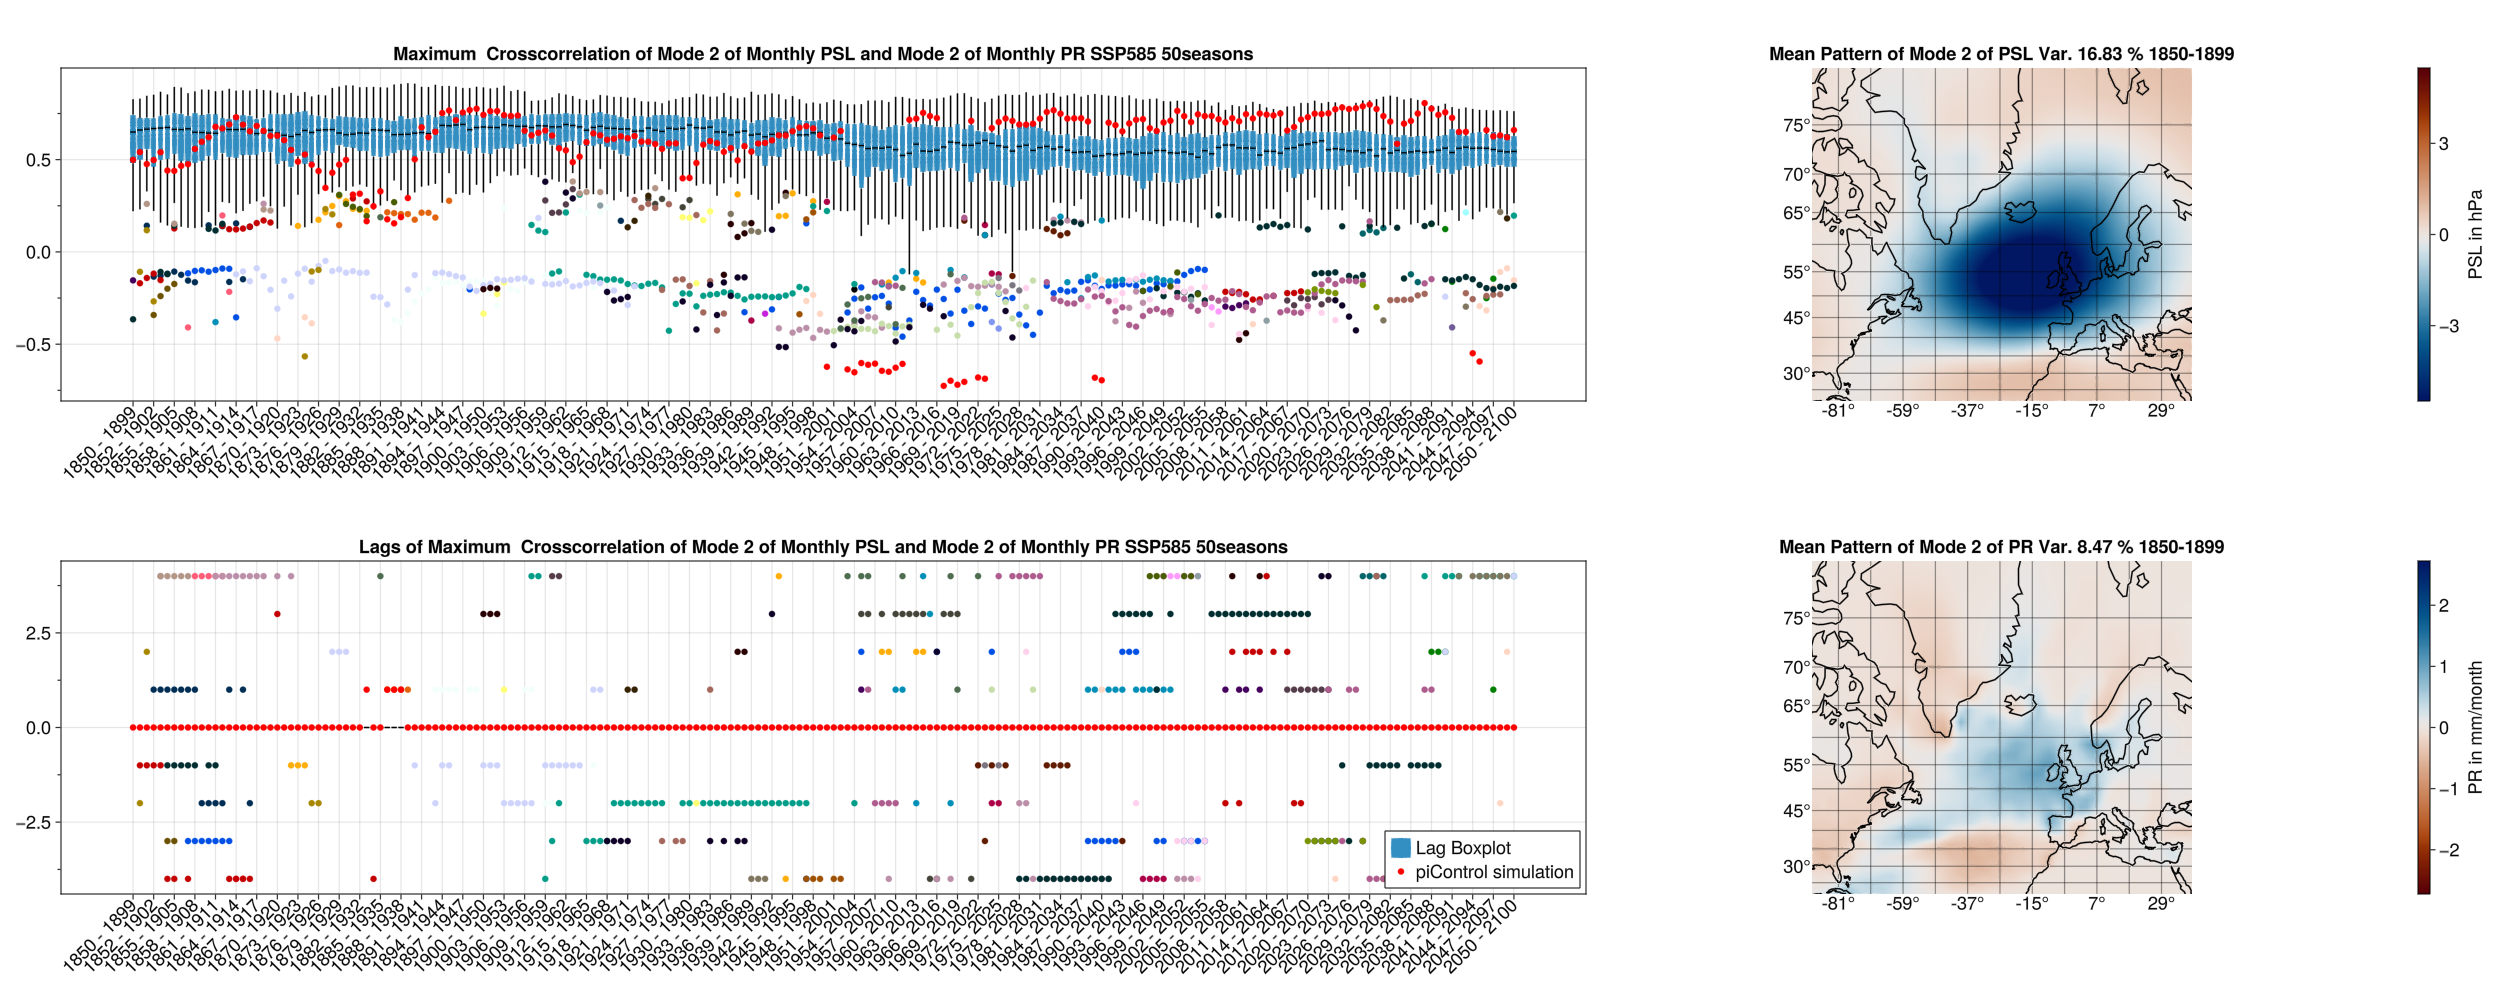
\includegraphics[width=0.95\textwidth]{figures/crosscorrelation_boxplot_psl_pr_modes22_ssp585_50seasons.png}
  \end{center}
  \caption{Same as Figure~\ref{fig:crosscor ivt psl modes11}, but with modes 2 of both Sea Level Pressure and precipitation EOFs.}\label{fig:crosscor psl pr modes22}

\end{figure}




\subsection{Relationships of EOFs with Variables}


\section{Discussion of Interpretation}
\label{sec:discussion}
